
\documentclass{article} % For LaTeX2e
\usepackage{iclr2027_conference,times}
% phi_pseudocode.tex
%王天虹 第一版
% In the main paper, load this file in the preamble with:
%   % phi_pseudocode.tex
%王天虹 第一版
% In the main paper, load this file in the preamble with:
%   % phi_pseudocode.tex
%王天虹 第一版
% In the main paper, load this file in the preamble with:
%   \input{phi_pseudocode.tex}
%
% and place:
%   \PHIPseudocode
% where the algorithm should appear.

\RequirePackage{algorithm}
\RequirePackage{algpseudocode}

\newcommand{\PHIPseudocode}{%
\begin{algorithm}[t]
\caption{Progressive Training and Causal Inference of PHI}
\label{alg:phi}
\footnotesize
\begin{algorithmic}[1]

\Require Demonstrations $\mathcal{D}$, future offsets
$\{\Delta_m\}_{m=1}^{M}$, force-history length $K$
\Ensure Trained causal policy $\pi$

% ============================================================
\Statex
\Statex \textbf{Stage I: Exploit privileged future information}

\For{each minibatch
$(I_t,\ell,s_t,F_{t-K+1:t},A_t^1,
\{I_{t+\Delta_m}\}_{m=1}^{M}) \sim \mathcal{D}$}

    \State $Z_t^{vl}
    \gets
    \operatorname{VLM}_{\bar{\omega}}(I_t,\ell)$

    \State $Z_t^{+}
    \gets
    R_{\psi}\!\left(
    E_v(I_{t+\Delta_1}),\ldots,E_v(I_{t+\Delta_M})
    \right)$

    \State $z_t^f
    \gets
    E_f\!\left(\phi(F_{t-K+1:t})\right)$,
    \quad
    $z_t^s \gets E_s(s_t)$

    \State Sample $A_t^0 \sim \mathcal{N}(0,I)$
    and $\tau \sim \mathcal{U}(0,1)$

    \State $A_t^\tau
    \gets
    (1-\tau)A_t^0+\tau A_t^1$,
    \quad
    $u_t \gets A_t^1-A_t^0$

    \State $\widehat{u}_t
    \gets
    G_{\theta}\!\left(
    A_t^\tau,\tau,
    Z_t^{vl},Z_t^{+},z_t^f,z_t^s
    \right)$

    \State $\mathcal{L}_{\mathrm{act}}
    \gets
    \left\|
    \widehat{u}_t-u_t
    \right\|_2^2$

    \State Update $\psi$, $E_f$, $E_s$, and $\theta$
    using $\mathcal{L}_{\mathrm{act}}$

\EndFor

% ============================================================
\Statex
\Statex \textbf{Stage II: Predict action-grounded future information}

\State Freeze all modules except $\operatorname{VLM}_{\omega}$

\For{each minibatch
$(I_t,\ell,\{I_{t+\Delta_m}\}_{m=1}^{M})
\sim\mathcal{D}$}

    \State $Z_t^{+}
    \gets
    R_{\psi}\!\left(
    E_v(I_{t+\Delta_1}),\ldots,E_v(I_{t+\Delta_M})
    \right)$

    \State $(Z_t^{vl},\widehat{Z}_t^{+})
    \gets
    \operatorname{VLM}_{\omega}(I_t,\ell)$

    \State $\mathcal{L}_{\mathrm{future}}
    \gets
    \left\|
    \widehat{Z}_t^{+}
    -
    \operatorname{sg}(Z_t^{+})
    \right\|_2^2$

    \State Update $\omega$
    using $\mathcal{L}_{\mathrm{future}}$

\EndFor

% ============================================================
\Statex
\Statex \textbf{Stage III: Align future prediction with action generation}

\State Unfreeze $\operatorname{VLM}_{\omega}$,
$E_f$, $E_s$, and $G_{\theta}$
\State Keep $R_{\psi}$ and $E_v$ frozen;
discard explicit future-latent supervision

\For{each minibatch
$(I_t,\ell,s_t,F_{t-K+1:t},A_t^1)
\sim\mathcal{D}$}

    \State $(Z_t^{vl},\widehat{Z}_t^{+})
    \gets
    \operatorname{VLM}_{\omega}(I_t,\ell)$

    \State $z_t^f
    \gets
    E_f\!\left(\phi(F_{t-K+1:t})\right)$,
    \quad
    $z_t^s \gets E_s(s_t)$

    \State Sample $A_t^0 \sim \mathcal{N}(0,I)$
    and $\tau \sim \mathcal{U}(0,1)$

    \State $A_t^\tau
    \gets
    (1-\tau)A_t^0+\tau A_t^1$,
    \quad
    $u_t \gets A_t^1-A_t^0$

    \State $\widehat{u}_t
    \gets
    G_{\theta}\!\left(
    A_t^\tau,\tau,
    Z_t^{vl},\widehat{Z}_t^{+},z_t^f,z_t^s
    \right)$

    \State $\mathcal{L}_{\mathrm{act}}
    \gets
    \left\|
    \widehat{u}_t-u_t
    \right\|_2^2$

    \State Jointly update $\omega$, $E_f$, $E_s$, and $\theta$
    using $\mathcal{L}_{\mathrm{act}}$

\EndFor

% ============================================================
\Statex
\Statex \textbf{Causal inference}

\For{each control step $t$}

    \State $(Z_t^{vl},\widehat{Z}_t^{+})
    \gets
    \operatorname{VLM}_{\omega}(I_t,\ell)$

    \State $z_t^f
    \gets
    E_f\!\left(\phi(F_{t-K+1:t})\right)$,
    \quad
    $z_t^s \gets E_s(s_t)$

    \State Sample $A_t^{\tau_0} \sim \mathcal{N}(0,I)$,
    where $\tau_0=0$

    \For{$n=0,\ldots,N-1$}

        \State $\widehat{u}_t^{\,n}
        \gets
        G_{\theta}\!\left(
        A_t^{\tau_n},\tau_n,
        Z_t^{vl},\widehat{Z}_t^{+},z_t^f,z_t^s
        \right)$

        \State $A_t^{\tau_{n+1}}
        \gets
        A_t^{\tau_n}
        +
        (\tau_{n+1}-\tau_n)\widehat{u}_t^{\,n}$

    \EndFor

    \State $A_t \gets A_t^{\tau_N}$

    \State Execute the first action(s) of $A_t$
    and update the observation history

\EndFor

\end{algorithmic}
\end{algorithm}%
}
%
% and place:
%   \PHIPseudocode
% where the algorithm should appear.

\RequirePackage{algorithm}
\RequirePackage{algpseudocode}

\newcommand{\PHIPseudocode}{%
\begin{algorithm}[t]
\caption{Progressive Training and Causal Inference of PHI}
\label{alg:phi}
\footnotesize
\begin{algorithmic}[1]

\Require Demonstrations $\mathcal{D}$, future offsets
$\{\Delta_m\}_{m=1}^{M}$, force-history length $K$
\Ensure Trained causal policy $\pi$

% ============================================================
\Statex
\Statex \textbf{Stage I: Exploit privileged future information}

\For{each minibatch
$(I_t,\ell,s_t,F_{t-K+1:t},A_t^1,
\{I_{t+\Delta_m}\}_{m=1}^{M}) \sim \mathcal{D}$}

    \State $Z_t^{vl}
    \gets
    \operatorname{VLM}_{\bar{\omega}}(I_t,\ell)$

    \State $Z_t^{+}
    \gets
    R_{\psi}\!\left(
    E_v(I_{t+\Delta_1}),\ldots,E_v(I_{t+\Delta_M})
    \right)$

    \State $z_t^f
    \gets
    E_f\!\left(\phi(F_{t-K+1:t})\right)$,
    \quad
    $z_t^s \gets E_s(s_t)$

    \State Sample $A_t^0 \sim \mathcal{N}(0,I)$
    and $\tau \sim \mathcal{U}(0,1)$

    \State $A_t^\tau
    \gets
    (1-\tau)A_t^0+\tau A_t^1$,
    \quad
    $u_t \gets A_t^1-A_t^0$

    \State $\widehat{u}_t
    \gets
    G_{\theta}\!\left(
    A_t^\tau,\tau,
    Z_t^{vl},Z_t^{+},z_t^f,z_t^s
    \right)$

    \State $\mathcal{L}_{\mathrm{act}}
    \gets
    \left\|
    \widehat{u}_t-u_t
    \right\|_2^2$

    \State Update $\psi$, $E_f$, $E_s$, and $\theta$
    using $\mathcal{L}_{\mathrm{act}}$

\EndFor

% ============================================================
\Statex
\Statex \textbf{Stage II: Predict action-grounded future information}

\State Freeze all modules except $\operatorname{VLM}_{\omega}$

\For{each minibatch
$(I_t,\ell,\{I_{t+\Delta_m}\}_{m=1}^{M})
\sim\mathcal{D}$}

    \State $Z_t^{+}
    \gets
    R_{\psi}\!\left(
    E_v(I_{t+\Delta_1}),\ldots,E_v(I_{t+\Delta_M})
    \right)$

    \State $(Z_t^{vl},\widehat{Z}_t^{+})
    \gets
    \operatorname{VLM}_{\omega}(I_t,\ell)$

    \State $\mathcal{L}_{\mathrm{future}}
    \gets
    \left\|
    \widehat{Z}_t^{+}
    -
    \operatorname{sg}(Z_t^{+})
    \right\|_2^2$

    \State Update $\omega$
    using $\mathcal{L}_{\mathrm{future}}$

\EndFor

% ============================================================
\Statex
\Statex \textbf{Stage III: Align future prediction with action generation}

\State Unfreeze $\operatorname{VLM}_{\omega}$,
$E_f$, $E_s$, and $G_{\theta}$
\State Keep $R_{\psi}$ and $E_v$ frozen;
discard explicit future-latent supervision

\For{each minibatch
$(I_t,\ell,s_t,F_{t-K+1:t},A_t^1)
\sim\mathcal{D}$}

    \State $(Z_t^{vl},\widehat{Z}_t^{+})
    \gets
    \operatorname{VLM}_{\omega}(I_t,\ell)$

    \State $z_t^f
    \gets
    E_f\!\left(\phi(F_{t-K+1:t})\right)$,
    \quad
    $z_t^s \gets E_s(s_t)$

    \State Sample $A_t^0 \sim \mathcal{N}(0,I)$
    and $\tau \sim \mathcal{U}(0,1)$

    \State $A_t^\tau
    \gets
    (1-\tau)A_t^0+\tau A_t^1$,
    \quad
    $u_t \gets A_t^1-A_t^0$

    \State $\widehat{u}_t
    \gets
    G_{\theta}\!\left(
    A_t^\tau,\tau,
    Z_t^{vl},\widehat{Z}_t^{+},z_t^f,z_t^s
    \right)$

    \State $\mathcal{L}_{\mathrm{act}}
    \gets
    \left\|
    \widehat{u}_t-u_t
    \right\|_2^2$

    \State Jointly update $\omega$, $E_f$, $E_s$, and $\theta$
    using $\mathcal{L}_{\mathrm{act}}$

\EndFor

% ============================================================
\Statex
\Statex \textbf{Causal inference}

\For{each control step $t$}

    \State $(Z_t^{vl},\widehat{Z}_t^{+})
    \gets
    \operatorname{VLM}_{\omega}(I_t,\ell)$

    \State $z_t^f
    \gets
    E_f\!\left(\phi(F_{t-K+1:t})\right)$,
    \quad
    $z_t^s \gets E_s(s_t)$

    \State Sample $A_t^{\tau_0} \sim \mathcal{N}(0,I)$,
    where $\tau_0=0$

    \For{$n=0,\ldots,N-1$}

        \State $\widehat{u}_t^{\,n}
        \gets
        G_{\theta}\!\left(
        A_t^{\tau_n},\tau_n,
        Z_t^{vl},\widehat{Z}_t^{+},z_t^f,z_t^s
        \right)$

        \State $A_t^{\tau_{n+1}}
        \gets
        A_t^{\tau_n}
        +
        (\tau_{n+1}-\tau_n)\widehat{u}_t^{\,n}$

    \EndFor

    \State $A_t \gets A_t^{\tau_N}$

    \State Execute the first action(s) of $A_t$
    and update the observation history

\EndFor

\end{algorithmic}
\end{algorithm}%
}
%
% and place:
%   \PHIPseudocode
% where the algorithm should appear.

\RequirePackage{algorithm}
\RequirePackage{algpseudocode}

\newcommand{\PHIPseudocode}{%
\begin{algorithm}[t]
\caption{Progressive Training and Causal Inference of PHI}
\label{alg:phi}
\footnotesize
\begin{algorithmic}[1]

\Require Demonstrations $\mathcal{D}$, future offsets
$\{\Delta_m\}_{m=1}^{M}$, force-history length $K$
\Ensure Trained causal policy $\pi$

% ============================================================
\Statex
\Statex \textbf{Stage I: Exploit privileged future information}

\For{each minibatch
$(I_t,\ell,s_t,F_{t-K+1:t},A_t^1,
\{I_{t+\Delta_m}\}_{m=1}^{M}) \sim \mathcal{D}$}

    \State $Z_t^{vl}
    \gets
    \operatorname{VLM}_{\bar{\omega}}(I_t,\ell)$

    \State $Z_t^{+}
    \gets
    R_{\psi}\!\left(
    E_v(I_{t+\Delta_1}),\ldots,E_v(I_{t+\Delta_M})
    \right)$

    \State $z_t^f
    \gets
    E_f\!\left(\phi(F_{t-K+1:t})\right)$,
    \quad
    $z_t^s \gets E_s(s_t)$

    \State Sample $A_t^0 \sim \mathcal{N}(0,I)$
    and $\tau \sim \mathcal{U}(0,1)$

    \State $A_t^\tau
    \gets
    (1-\tau)A_t^0+\tau A_t^1$,
    \quad
    $u_t \gets A_t^1-A_t^0$

    \State $\widehat{u}_t
    \gets
    G_{\theta}\!\left(
    A_t^\tau,\tau,
    Z_t^{vl},Z_t^{+},z_t^f,z_t^s
    \right)$

    \State $\mathcal{L}_{\mathrm{act}}
    \gets
    \left\|
    \widehat{u}_t-u_t
    \right\|_2^2$

    \State Update $\psi$, $E_f$, $E_s$, and $\theta$
    using $\mathcal{L}_{\mathrm{act}}$

\EndFor

% ============================================================
\Statex
\Statex \textbf{Stage II: Predict action-grounded future information}

\State Freeze all modules except $\operatorname{VLM}_{\omega}$

\For{each minibatch
$(I_t,\ell,\{I_{t+\Delta_m}\}_{m=1}^{M})
\sim\mathcal{D}$}

    \State $Z_t^{+}
    \gets
    R_{\psi}\!\left(
    E_v(I_{t+\Delta_1}),\ldots,E_v(I_{t+\Delta_M})
    \right)$

    \State $(Z_t^{vl},\widehat{Z}_t^{+})
    \gets
    \operatorname{VLM}_{\omega}(I_t,\ell)$

    \State $\mathcal{L}_{\mathrm{future}}
    \gets
    \left\|
    \widehat{Z}_t^{+}
    -
    \operatorname{sg}(Z_t^{+})
    \right\|_2^2$

    \State Update $\omega$
    using $\mathcal{L}_{\mathrm{future}}$

\EndFor

% ============================================================
\Statex
\Statex \textbf{Stage III: Align future prediction with action generation}

\State Unfreeze $\operatorname{VLM}_{\omega}$,
$E_f$, $E_s$, and $G_{\theta}$
\State Keep $R_{\psi}$ and $E_v$ frozen;
discard explicit future-latent supervision

\For{each minibatch
$(I_t,\ell,s_t,F_{t-K+1:t},A_t^1)
\sim\mathcal{D}$}

    \State $(Z_t^{vl},\widehat{Z}_t^{+})
    \gets
    \operatorname{VLM}_{\omega}(I_t,\ell)$

    \State $z_t^f
    \gets
    E_f\!\left(\phi(F_{t-K+1:t})\right)$,
    \quad
    $z_t^s \gets E_s(s_t)$

    \State Sample $A_t^0 \sim \mathcal{N}(0,I)$
    and $\tau \sim \mathcal{U}(0,1)$

    \State $A_t^\tau
    \gets
    (1-\tau)A_t^0+\tau A_t^1$,
    \quad
    $u_t \gets A_t^1-A_t^0$

    \State $\widehat{u}_t
    \gets
    G_{\theta}\!\left(
    A_t^\tau,\tau,
    Z_t^{vl},\widehat{Z}_t^{+},z_t^f,z_t^s
    \right)$

    \State $\mathcal{L}_{\mathrm{act}}
    \gets
    \left\|
    \widehat{u}_t-u_t
    \right\|_2^2$

    \State Jointly update $\omega$, $E_f$, $E_s$, and $\theta$
    using $\mathcal{L}_{\mathrm{act}}$

\EndFor

% ============================================================
\Statex
\Statex \textbf{Causal inference}

\For{each control step $t$}

    \State $(Z_t^{vl},\widehat{Z}_t^{+})
    \gets
    \operatorname{VLM}_{\omega}(I_t,\ell)$

    \State $z_t^f
    \gets
    E_f\!\left(\phi(F_{t-K+1:t})\right)$,
    \quad
    $z_t^s \gets E_s(s_t)$

    \State Sample $A_t^{\tau_0} \sim \mathcal{N}(0,I)$,
    where $\tau_0=0$

    \For{$n=0,\ldots,N-1$}

        \State $\widehat{u}_t^{\,n}
        \gets
        G_{\theta}\!\left(
        A_t^{\tau_n},\tau_n,
        Z_t^{vl},\widehat{Z}_t^{+},z_t^f,z_t^s
        \right)$

        \State $A_t^{\tau_{n+1}}
        \gets
        A_t^{\tau_n}
        +
        (\tau_{n+1}-\tau_n)\widehat{u}_t^{\,n}$

    \EndFor

    \State $A_t \gets A_t^{\tau_N}$

    \State Execute the first action(s) of $A_t$
    and update the observation history

\EndFor

\end{algorithmic}
\end{algorithm}%
}
% Optional math commands from https://github.com/goodfeli/dlbook_notation
\setlength{\textfloatsep}{8pt plus 2pt minus 2pt}

\usepackage{tabularx}
\usepackage{caption}
\usepackage{needspace}
\usepackage{wrapfig}
\usepackage{hyperref}
\usepackage{url}
\usepackage{booktabs} 
\usepackage{graphicx} 
\usepackage{colortbl}
\usepackage{wrapfig}
%%%%% NEW MATH DEFINITIONS %%%%%

\usepackage{amsmath,amsfonts,bm}

% Mark sections of captions for referring to divisions of figures
\newcommand{\figleft}{{\em (Left)}}
\newcommand{\figcenter}{{\em (Center)}}
\newcommand{\figright}{{\em (Right)}}
\newcommand{\figtop}{{\em (Top)}}
\newcommand{\figbottom}{{\em (Bottom)}}
\newcommand{\captiona}{{\em (a)}}
\newcommand{\captionb}{{\em (b)}}
\newcommand{\captionc}{{\em (c)}}
\newcommand{\captiond}{{\em (d)}}

% Highlight a newly defined term
\newcommand{\newterm}[1]{{\bf #1}}


% Figure reference, lower-case.
\def\figref#1{figure~\ref{#1}}
% Figure reference, capital. For start of sentence
\def\Figref#1{Figure~\ref{#1}}
\def\twofigref#1#2{figures \ref{#1} and \ref{#2}}
\def\quadfigref#1#2#3#4{figures \ref{#1}, \ref{#2}, \ref{#3} and \ref{#4}}
% Section reference, lower-case.
\def\secref#1{section~\ref{#1}}
% Section reference, capital.
\def\Secref#1{Section~\ref{#1}}
% Reference to two sections.
\def\twosecrefs#1#2{sections \ref{#1} and \ref{#2}}
% Reference to three sections.
\def\secrefs#1#2#3{sections \ref{#1}, \ref{#2} and \ref{#3}}
% Reference to an equation, lower-case.
\def\eqref#1{equation~\ref{#1}}
% Reference to an equation, upper case
\def\Eqref#1{Equation~\ref{#1}}
% A raw reference to an equation---avoid using if possible
\def\plaineqref#1{\ref{#1}}
% Reference to a chapter, lower-case.
\def\chapref#1{chapter~\ref{#1}}
% Reference to an equation, upper case.
\def\Chapref#1{Chapter~\ref{#1}}
% Reference to a range of chapters
\def\rangechapref#1#2{chapters\ref{#1}--\ref{#2}}
% Reference to an algorithm, lower-case.
\def\algref#1{algorithm~\ref{#1}}
% Reference to an algorithm, upper case.
\def\Algref#1{Algorithm~\ref{#1}}
\def\twoalgref#1#2{algorithms \ref{#1} and \ref{#2}}
\def\Twoalgref#1#2{Algorithms \ref{#1} and \ref{#2}}
% Reference to a part, lower case
\def\partref#1{part~\ref{#1}}
% Reference to a part, upper case
\def\Partref#1{Part~\ref{#1}}
\def\twopartref#1#2{parts \ref{#1} and \ref{#2}}

\def\ceil#1{\lceil #1 \rceil}
\def\floor#1{\lfloor #1 \rfloor}
\def\1{\bm{1}}
\newcommand{\train}{\mathcal{D}}
\newcommand{\valid}{\mathcal{D_{\mathrm{valid}}}}
\newcommand{\test}{\mathcal{D_{\mathrm{test}}}}

\def\eps{{\epsilon}}


% Random variables
\def\reta{{\textnormal{$\eta$}}}
\def\ra{{\textnormal{a}}}
\def\rb{{\textnormal{b}}}
\def\rc{{\textnormal{c}}}
\def\rd{{\textnormal{d}}}
\def\re{{\textnormal{e}}}
\def\rf{{\textnormal{f}}}
\def\rg{{\textnormal{g}}}
\def\rh{{\textnormal{h}}}
\def\ri{{\textnormal{i}}}
\def\rj{{\textnormal{j}}}
\def\rk{{\textnormal{k}}}
\def\rl{{\textnormal{l}}}
% rm is already a command, just don't name any random variables m
\def\rn{{\textnormal{n}}}
\def\ro{{\textnormal{o}}}
\def\rp{{\textnormal{p}}}
\def\rq{{\textnormal{q}}}
\def\rr{{\textnormal{r}}}
\def\rs{{\textnormal{s}}}
\def\rt{{\textnormal{t}}}
\def\ru{{\textnormal{u}}}
\def\rv{{\textnormal{v}}}
\def\rw{{\textnormal{w}}}
\def\rx{{\textnormal{x}}}
\def\ry{{\textnormal{y}}}
\def\rz{{\textnormal{z}}}

% Random vectors
\def\rvepsilon{{\mathbf{\epsilon}}}
\def\rvtheta{{\mathbf{\theta}}}
\def\rva{{\mathbf{a}}}
\def\rvb{{\mathbf{b}}}
\def\rvc{{\mathbf{c}}}
\def\rvd{{\mathbf{d}}}
\def\rve{{\mathbf{e}}}
\def\rvf{{\mathbf{f}}}
\def\rvg{{\mathbf{g}}}
\def\rvh{{\mathbf{h}}}
\def\rvu{{\mathbf{i}}}
\def\rvj{{\mathbf{j}}}
\def\rvk{{\mathbf{k}}}
\def\rvl{{\mathbf{l}}}
\def\rvm{{\mathbf{m}}}
\def\rvn{{\mathbf{n}}}
\def\rvo{{\mathbf{o}}}
\def\rvp{{\mathbf{p}}}
\def\rvq{{\mathbf{q}}}
\def\rvr{{\mathbf{r}}}
\def\rvs{{\mathbf{s}}}
\def\rvt{{\mathbf{t}}}
\def\rvu{{\mathbf{u}}}
\def\rvv{{\mathbf{v}}}
\def\rvw{{\mathbf{w}}}
\def\rvx{{\mathbf{x}}}
\def\rvy{{\mathbf{y}}}
\def\rvz{{\mathbf{z}}}

% Elements of random vectors
\def\erva{{\textnormal{a}}}
\def\ervb{{\textnormal{b}}}
\def\ervc{{\textnormal{c}}}
\def\ervd{{\textnormal{d}}}
\def\erve{{\textnormal{e}}}
\def\ervf{{\textnormal{f}}}
\def\ervg{{\textnormal{g}}}
\def\ervh{{\textnormal{h}}}
\def\ervi{{\textnormal{i}}}
\def\ervj{{\textnormal{j}}}
\def\ervk{{\textnormal{k}}}
\def\ervl{{\textnormal{l}}}
\def\ervm{{\textnormal{m}}}
\def\ervn{{\textnormal{n}}}
\def\ervo{{\textnormal{o}}}
\def\ervp{{\textnormal{p}}}
\def\ervq{{\textnormal{q}}}
\def\ervr{{\textnormal{r}}}
\def\ervs{{\textnormal{s}}}
\def\ervt{{\textnormal{t}}}
\def\ervu{{\textnormal{u}}}
\def\ervv{{\textnormal{v}}}
\def\ervw{{\textnormal{w}}}
\def\ervx{{\textnormal{x}}}
\def\ervy{{\textnormal{y}}}
\def\ervz{{\textnormal{z}}}

% Random matrices
\def\rmA{{\mathbf{A}}}
\def\rmB{{\mathbf{B}}}
\def\rmC{{\mathbf{C}}}
\def\rmD{{\mathbf{D}}}
\def\rmE{{\mathbf{E}}}
\def\rmF{{\mathbf{F}}}
\def\rmG{{\mathbf{G}}}
\def\rmH{{\mathbf{H}}}
\def\rmI{{\mathbf{I}}}
\def\rmJ{{\mathbf{J}}}
\def\rmK{{\mathbf{K}}}
\def\rmL{{\mathbf{L}}}
\def\rmM{{\mathbf{M}}}
\def\rmN{{\mathbf{N}}}
\def\rmO{{\mathbf{O}}}
\def\rmP{{\mathbf{P}}}
\def\rmQ{{\mathbf{Q}}}
\def\rmR{{\mathbf{R}}}
\def\rmS{{\mathbf{S}}}
\def\rmT{{\mathbf{T}}}
\def\rmU{{\mathbf{U}}}
\def\rmV{{\mathbf{V}}}
\def\rmW{{\mathbf{W}}}
\def\rmX{{\mathbf{X}}}
\def\rmY{{\mathbf{Y}}}
\def\rmZ{{\mathbf{Z}}}

% Elements of random matrices
\def\ermA{{\textnormal{A}}}
\def\ermB{{\textnormal{B}}}
\def\ermC{{\textnormal{C}}}
\def\ermD{{\textnormal{D}}}
\def\ermE{{\textnormal{E}}}
\def\ermF{{\textnormal{F}}}
\def\ermG{{\textnormal{G}}}
\def\ermH{{\textnormal{H}}}
\def\ermI{{\textnormal{I}}}
\def\ermJ{{\textnormal{J}}}
\def\ermK{{\textnormal{K}}}
\def\ermL{{\textnormal{L}}}
\def\ermM{{\textnormal{M}}}
\def\ermN{{\textnormal{N}}}
\def\ermO{{\textnormal{O}}}
\def\ermP{{\textnormal{P}}}
\def\ermQ{{\textnormal{Q}}}
\def\ermR{{\textnormal{R}}}
\def\ermS{{\textnormal{S}}}
\def\ermT{{\textnormal{T}}}
\def\ermU{{\textnormal{U}}}
\def\ermV{{\textnormal{V}}}
\def\ermW{{\textnormal{W}}}
\def\ermX{{\textnormal{X}}}
\def\ermY{{\textnormal{Y}}}
\def\ermZ{{\textnormal{Z}}}

% Vectors
\def\vzero{{\bm{0}}}
\def\vone{{\bm{1}}}
\def\vmu{{\bm{\mu}}}
\def\vtheta{{\bm{\theta}}}
\def\va{{\bm{a}}}
\def\vb{{\bm{b}}}
\def\vc{{\bm{c}}}
\def\vd{{\bm{d}}}
\def\ve{{\bm{e}}}
\def\vf{{\bm{f}}}
\def\vg{{\bm{g}}}
\def\vh{{\bm{h}}}
\def\vi{{\bm{i}}}
\def\vj{{\bm{j}}}
\def\vk{{\bm{k}}}
\def\vl{{\bm{l}}}
\def\vm{{\bm{m}}}
\def\vn{{\bm{n}}}
\def\vo{{\bm{o}}}
\def\vp{{\bm{p}}}
\def\vq{{\bm{q}}}
\def\vr{{\bm{r}}}
\def\vs{{\bm{s}}}
\def\vt{{\bm{t}}}
\def\vu{{\bm{u}}}
\def\vv{{\bm{v}}}
\def\vw{{\bm{w}}}
\def\vx{{\bm{x}}}
\def\vy{{\bm{y}}}
\def\vz{{\bm{z}}}

% Elements of vectors
\def\evalpha{{\alpha}}
\def\evbeta{{\beta}}
\def\evepsilon{{\epsilon}}
\def\evlambda{{\lambda}}
\def\evomega{{\omega}}
\def\evmu{{\mu}}
\def\evpsi{{\psi}}
\def\evsigma{{\sigma}}
\def\evtheta{{\theta}}
\def\eva{{a}}
\def\evb{{b}}
\def\evc{{c}}
\def\evd{{d}}
\def\eve{{e}}
\def\evf{{f}}
\def\evg{{g}}
\def\evh{{h}}
\def\evi{{i}}
\def\evj{{j}}
\def\evk{{k}}
\def\evl{{l}}
\def\evm{{m}}
\def\evn{{n}}
\def\evo{{o}}
\def\evp{{p}}
\def\evq{{q}}
\def\evr{{r}}
\def\evs{{s}}
\def\evt{{t}}
\def\evu{{u}}
\def\evv{{v}}
\def\evw{{w}}
\def\evx{{x}}
\def\evy{{y}}
\def\evz{{z}}

% Matrix
\def\mA{{\bm{A}}}
\def\mB{{\bm{B}}}
\def\mC{{\bm{C}}}
\def\mD{{\bm{D}}}
\def\mE{{\bm{E}}}
\def\mF{{\bm{F}}}
\def\mG{{\bm{G}}}
\def\mH{{\bm{H}}}
\def\mI{{\bm{I}}}
\def\mJ{{\bm{J}}}
\def\mK{{\bm{K}}}
\def\mL{{\bm{L}}}
\def\mM{{\bm{M}}}
\def\mN{{\bm{N}}}
\def\mO{{\bm{O}}}
\def\mP{{\bm{P}}}
\def\mQ{{\bm{Q}}}
\def\mR{{\bm{R}}}
\def\mS{{\bm{S}}}
\def\mT{{\bm{T}}}
\def\mU{{\bm{U}}}
\def\mV{{\bm{V}}}
\def\mW{{\bm{W}}}
\def\mX{{\bm{X}}}
\def\mY{{\bm{Y}}}
\def\mZ{{\bm{Z}}}
\def\mBeta{{\bm{\beta}}}
\def\mPhi{{\bm{\Phi}}}
\def\mLambda{{\bm{\Lambda}}}
\def\mSigma{{\bm{\Sigma}}}

% Tensor
\DeclareMathAlphabet{\mathsfit}{\encodingdefault}{\sfdefault}{m}{sl}
\SetMathAlphabet{\mathsfit}{bold}{\encodingdefault}{\sfdefault}{bx}{n}
\newcommand{\tens}[1]{\bm{\mathsfit{#1}}}
\def\tA{{\tens{A}}}
\def\tB{{\tens{B}}}
\def\tC{{\tens{C}}}
\def\tD{{\tens{D}}}
\def\tE{{\tens{E}}}
\def\tF{{\tens{F}}}
\def\tG{{\tens{G}}}
\def\tH{{\tens{H}}}
\def\tI{{\tens{I}}}
\def\tJ{{\tens{J}}}
\def\tK{{\tens{K}}}
\def\tL{{\tens{L}}}
\def\tM{{\tens{M}}}
\def\tN{{\tens{N}}}
\def\tO{{\tens{O}}}
\def\tP{{\tens{P}}}
\def\tQ{{\tens{Q}}}
\def\tR{{\tens{R}}}
\def\tS{{\tens{S}}}
\def\tT{{\tens{T}}}
\def\tU{{\tens{U}}}
\def\tV{{\tens{V}}}
\def\tW{{\tens{W}}}
\def\tX{{\tens{X}}}
\def\tY{{\tens{Y}}}
\def\tZ{{\tens{Z}}}


% Graph
\def\gA{{\mathcal{A}}}
\def\gB{{\mathcal{B}}}
\def\gC{{\mathcal{C}}}
\def\gD{{\mathcal{D}}}
\def\gE{{\mathcal{E}}}
\def\gF{{\mathcal{F}}}
\def\gG{{\mathcal{G}}}
\def\gH{{\mathcal{H}}}
\def\gI{{\mathcal{I}}}
\def\gJ{{\mathcal{J}}}
\def\gK{{\mathcal{K}}}
\def\gL{{\mathcal{L}}}
\def\gM{{\mathcal{M}}}
\def\gN{{\mathcal{N}}}
\def\gO{{\mathcal{O}}}
\def\gP{{\mathcal{P}}}
\def\gQ{{\mathcal{Q}}}
\def\gR{{\mathcal{R}}}
\def\gS{{\mathcal{S}}}
\def\gT{{\mathcal{T}}}
\def\gU{{\mathcal{U}}}
\def\gV{{\mathcal{V}}}
\def\gW{{\mathcal{W}}}
\def\gX{{\mathcal{X}}}
\def\gY{{\mathcal{Y}}}
\def\gZ{{\mathcal{Z}}}

% Sets
\def\sA{{\mathbb{A}}}
\def\sB{{\mathbb{B}}}
\def\sC{{\mathbb{C}}}
\def\sD{{\mathbb{D}}}
% Don't use a set called E, because this would be the same as our symbol
% for expectation.
\def\sF{{\mathbb{F}}}
\def\sG{{\mathbb{G}}}
\def\sH{{\mathbb{H}}}
\def\sI{{\mathbb{I}}}
\def\sJ{{\mathbb{J}}}
\def\sK{{\mathbb{K}}}
\def\sL{{\mathbb{L}}}
\def\sM{{\mathbb{M}}}
\def\sN{{\mathbb{N}}}
\def\sO{{\mathbb{O}}}
\def\sP{{\mathbb{P}}}
\def\sQ{{\mathbb{Q}}}
\def\sR{{\mathbb{R}}}
\def\sS{{\mathbb{S}}}
\def\sT{{\mathbb{T}}}
\def\sU{{\mathbb{U}}}
\def\sV{{\mathbb{V}}}
\def\sW{{\mathbb{W}}}
\def\sX{{\mathbb{X}}}
\def\sY{{\mathbb{Y}}}
\def\sZ{{\mathbb{Z}}}

% Entries of a matrix
\def\emLambda{{\Lambda}}
\def\emA{{A}}
\def\emB{{B}}
\def\emC{{C}}
\def\emD{{D}}
\def\emE{{E}}
\def\emF{{F}}
\def\emG{{G}}
\def\emH{{H}}
\def\emI{{I}}
\def\emJ{{J}}
\def\emK{{K}}
\def\emL{{L}}
\def\emM{{M}}
\def\emN{{N}}
\def\emO{{O}}
\def\emP{{P}}
\def\emQ{{Q}}
\def\emR{{R}}
\def\emS{{S}}
\def\emT{{T}}
\def\emU{{U}}
\def\emV{{V}}
\def\emW{{W}}
\def\emX{{X}}
\def\emY{{Y}}
\def\emZ{{Z}}
\def\emSigma{{\Sigma}}

% entries of a tensor
% Same font as tensor, without \bm wrapper
\newcommand{\etens}[1]{\mathsfit{#1}}
\def\etLambda{{\etens{\Lambda}}}
\def\etA{{\etens{A}}}
\def\etB{{\etens{B}}}
\def\etC{{\etens{C}}}
\def\etD{{\etens{D}}}
\def\etE{{\etens{E}}}
\def\etF{{\etens{F}}}
\def\etG{{\etens{G}}}
\def\etH{{\etens{H}}}
\def\etI{{\etens{I}}}
\def\etJ{{\etens{J}}}
\def\etK{{\etens{K}}}
\def\etL{{\etens{L}}}
\def\etM{{\etens{M}}}
\def\etN{{\etens{N}}}
\def\etO{{\etens{O}}}
\def\etP{{\etens{P}}}
\def\etQ{{\etens{Q}}}
\def\etR{{\etens{R}}}
\def\etS{{\etens{S}}}
\def\etT{{\etens{T}}}
\def\etU{{\etens{U}}}
\def\etV{{\etens{V}}}
\def\etW{{\etens{W}}}
\def\etX{{\etens{X}}}
\def\etY{{\etens{Y}}}
\def\etZ{{\etens{Z}}}

% The true underlying data generating distribution
\newcommand{\pdata}{p_{\rm{data}}}
% The empirical distribution defined by the training set
\newcommand{\ptrain}{\hat{p}_{\rm{data}}}
\newcommand{\Ptrain}{\hat{P}_{\rm{data}}}
% The model distribution
\newcommand{\pmodel}{p_{\rm{model}}}
\newcommand{\Pmodel}{P_{\rm{model}}}
\newcommand{\ptildemodel}{\tilde{p}_{\rm{model}}}
% Stochastic autoencoder distributions
\newcommand{\pencode}{p_{\rm{encoder}}}
\newcommand{\pdecode}{p_{\rm{decoder}}}
\newcommand{\precons}{p_{\rm{reconstruct}}}

\newcommand{\laplace}{\mathrm{Laplace}} % Laplace distribution

\newcommand{\E}{\mathbb{E}}
\newcommand{\Ls}{\mathcal{L}}
\newcommand{\R}{\mathbb{R}}
\newcommand{\emp}{\tilde{p}}
\newcommand{\lr}{\alpha}
\newcommand{\reg}{\lambda}
\newcommand{\rect}{\mathrm{rectifier}}
\newcommand{\softmax}{\mathrm{softmax}}
\newcommand{\sigmoid}{\sigma}
\newcommand{\softplus}{\zeta}
\newcommand{\KL}{D_{\mathrm{KL}}}
\newcommand{\Var}{\mathrm{Var}}
\newcommand{\standarderror}{\mathrm{SE}}
\newcommand{\Cov}{\mathrm{Cov}}
% Wolfram Mathworld says $L^2$ is for function spaces and $\ell^2$ is for vectors
% But then they seem to use $L^2$ for vectors throughout the site, and so does
% wikipedia.
\newcommand{\normlzero}{L^0}
\newcommand{\normlone}{L^1}
\newcommand{\normltwo}{L^2}
\newcommand{\normlp}{L^p}
\newcommand{\normmax}{L^\infty}

\newcommand{\parents}{Pa} % See usage in notation.tex. Chosen to match Daphne's book.

\DeclareMathOperator*{\argmax}{arg\,max}
\DeclareMathOperator*{\argmin}{arg\,min}

\DeclareMathOperator{\sign}{sign}
\DeclareMathOperator{\Tr}{Tr}
\let\ab\allowbreak

\title{PHI: A Hierarchical World Action Model with Selective Prediction and Force Feedback for Humanoid Bimanual Manipulation}

% Authors must not appear in the submitted version. They should be hidden
% as long as the \iclrfinalcopy macro remains commented out below.
% Non-anonymous submissions will be rejected without review.

\author{Antiquus S.~Hippocampus, Natalia Cerebro \& Amelie P. Amygdale \thanks{ Use footnote for providing further information
about author (webpage, alternative address)---\emph{not} for acknowledging
funding agencies.  Funding acknowledgements go at the end of the paper.} \\
Department of Computer Science\\
Cranberry-Lemon University\\
Pittsburgh, PA 15213, USA \\
\texttt{\{hippo,brain,jen\}@cs.cranberry-lemon.edu} \\
\And
Ji Q. Ren \& Yevgeny LeNet \\
Department of Computational Neuroscience \\
University of the Witwatersrand \\
Joburg, South Africa \\
\texttt{\{robot,net\}@wits.ac.za} \\
\AND
Coauthor \\
Affiliation \\
Address \\
\texttt{email}
}

% The \author macro works with any number of authors. There are two commands
% used to separate the names and addresses of multiple authors: \And and \AND.
%
% Using \And between authors leaves it to \LaTeX{} to determine where to break
% the lines. Using \AND forces a linebreak at that point. So, if \LaTeX{}
% puts 3 of 4 authors names on the first line, and the last on the second
% line, try using \AND instead of \And before the third author name.

\newcommand{\fix}{\marginpar{FIX}}
\newcommand{\new}{\marginpar{NEW}}

%\iclrfinalcopy % Uncomment for camera-ready version, but NOT for submission.
\begin{document}
\setlength{\floatsep}{6pt plus 2pt minus 2pt}.

\maketitle

% \begin{center}
% \href{https://phi-wam.github.io/}{Project Page}
% \end{center}

\begin{abstract}

Humanoid bimanual dexterous manipulation requires coordinated dual-arm and finger actions under evolving contact interactions. Existing world action models (WAMs) offer a promising way to model such future dynamics, but primarily optimize future representations for prediction, leaving their utility for downstream action generation implicit. We introduce \textbf{PHI} (Predictive Hierarchical Intelligence), a \textbf{hierarchical world action model} for humanoid bimanual manipulation that integrates \textbf{selective future prediction} with \textbf{force feedback}. Rather than reconstructing or preserving the complete future observation, PHI selectively learns compact future visual representations that retain information useful for action generation. A hierarchical predictive pathway first extracts task-relevant future representations from privileged future observations during training and then learns to infer them from the current interaction context at deployment. To complement visual prediction in contact-rich interactions, PHI further incorporates a temporal force encoder that captures recent force evolution and provides physical feedback about contact establishment, loading, and interaction changes. The predicted future representation and force feedback are jointly integrated to guide action generation. Across five real-world humanoid bimanual manipulation tasks, PHI achieves an aggregate success rate of 82.0\%, outperforming the strongest baseline by 23.3 percentage points and up to a 30.0 percentage points gain on unseen book instances. These results demonstrate PHI's effectiveness through selective future prediction and temporal force feedback. \href{https://phi-wam.github.io/}{PHI-WAM}.





% Humanoid bimanual dexterous manipulation is particularly challenging because robots must coordinate dual-arm motions and fine-grained finger actions while reasoning about coupled physical interactions that evolve through contact. Anticipating these interaction dynamics is critical for deciding how to act as contact conditions change. Existing world action models (WAMs) offer a promising way to model such future dynamics, but primarily optimize future representations for prediction, leaving their utility for downstream action generation implicit. We introduce \textbf{PHI} (Predictive Hierarchical Intelligence), denoted as $\Phi$, a task oriented world model that learns future representations explicitly shaped by their usefulness for action generation. $\Phi$ first learns task-relevant future visual representations and then trains a WAM to infer them from the current interaction context. To capture contact dynamics that are difficult to infer from vision alone, $\Phi$ further encodes recent force evolution with a temporal force module. The predicted future visual representation and force representation jointly guide action generation. Across five real-world humanoid manipulation tasks, $\Phi$ consistently outperforms strong generalist baselines, achieving a higher aggregate success rate than the baseline, corresponding to a $23.3\%$ improvement. Under generalization to unseen books, $\Phi$ further improves success rates by up to $30.0$ percentage points over the strongest baseline. These results demonstrate the effectiveness of learning compact, task oriented predictive representations together with temporal force information for robust humanoid manipulation.





\end{abstract}


\begin{figure}[th]
\centering
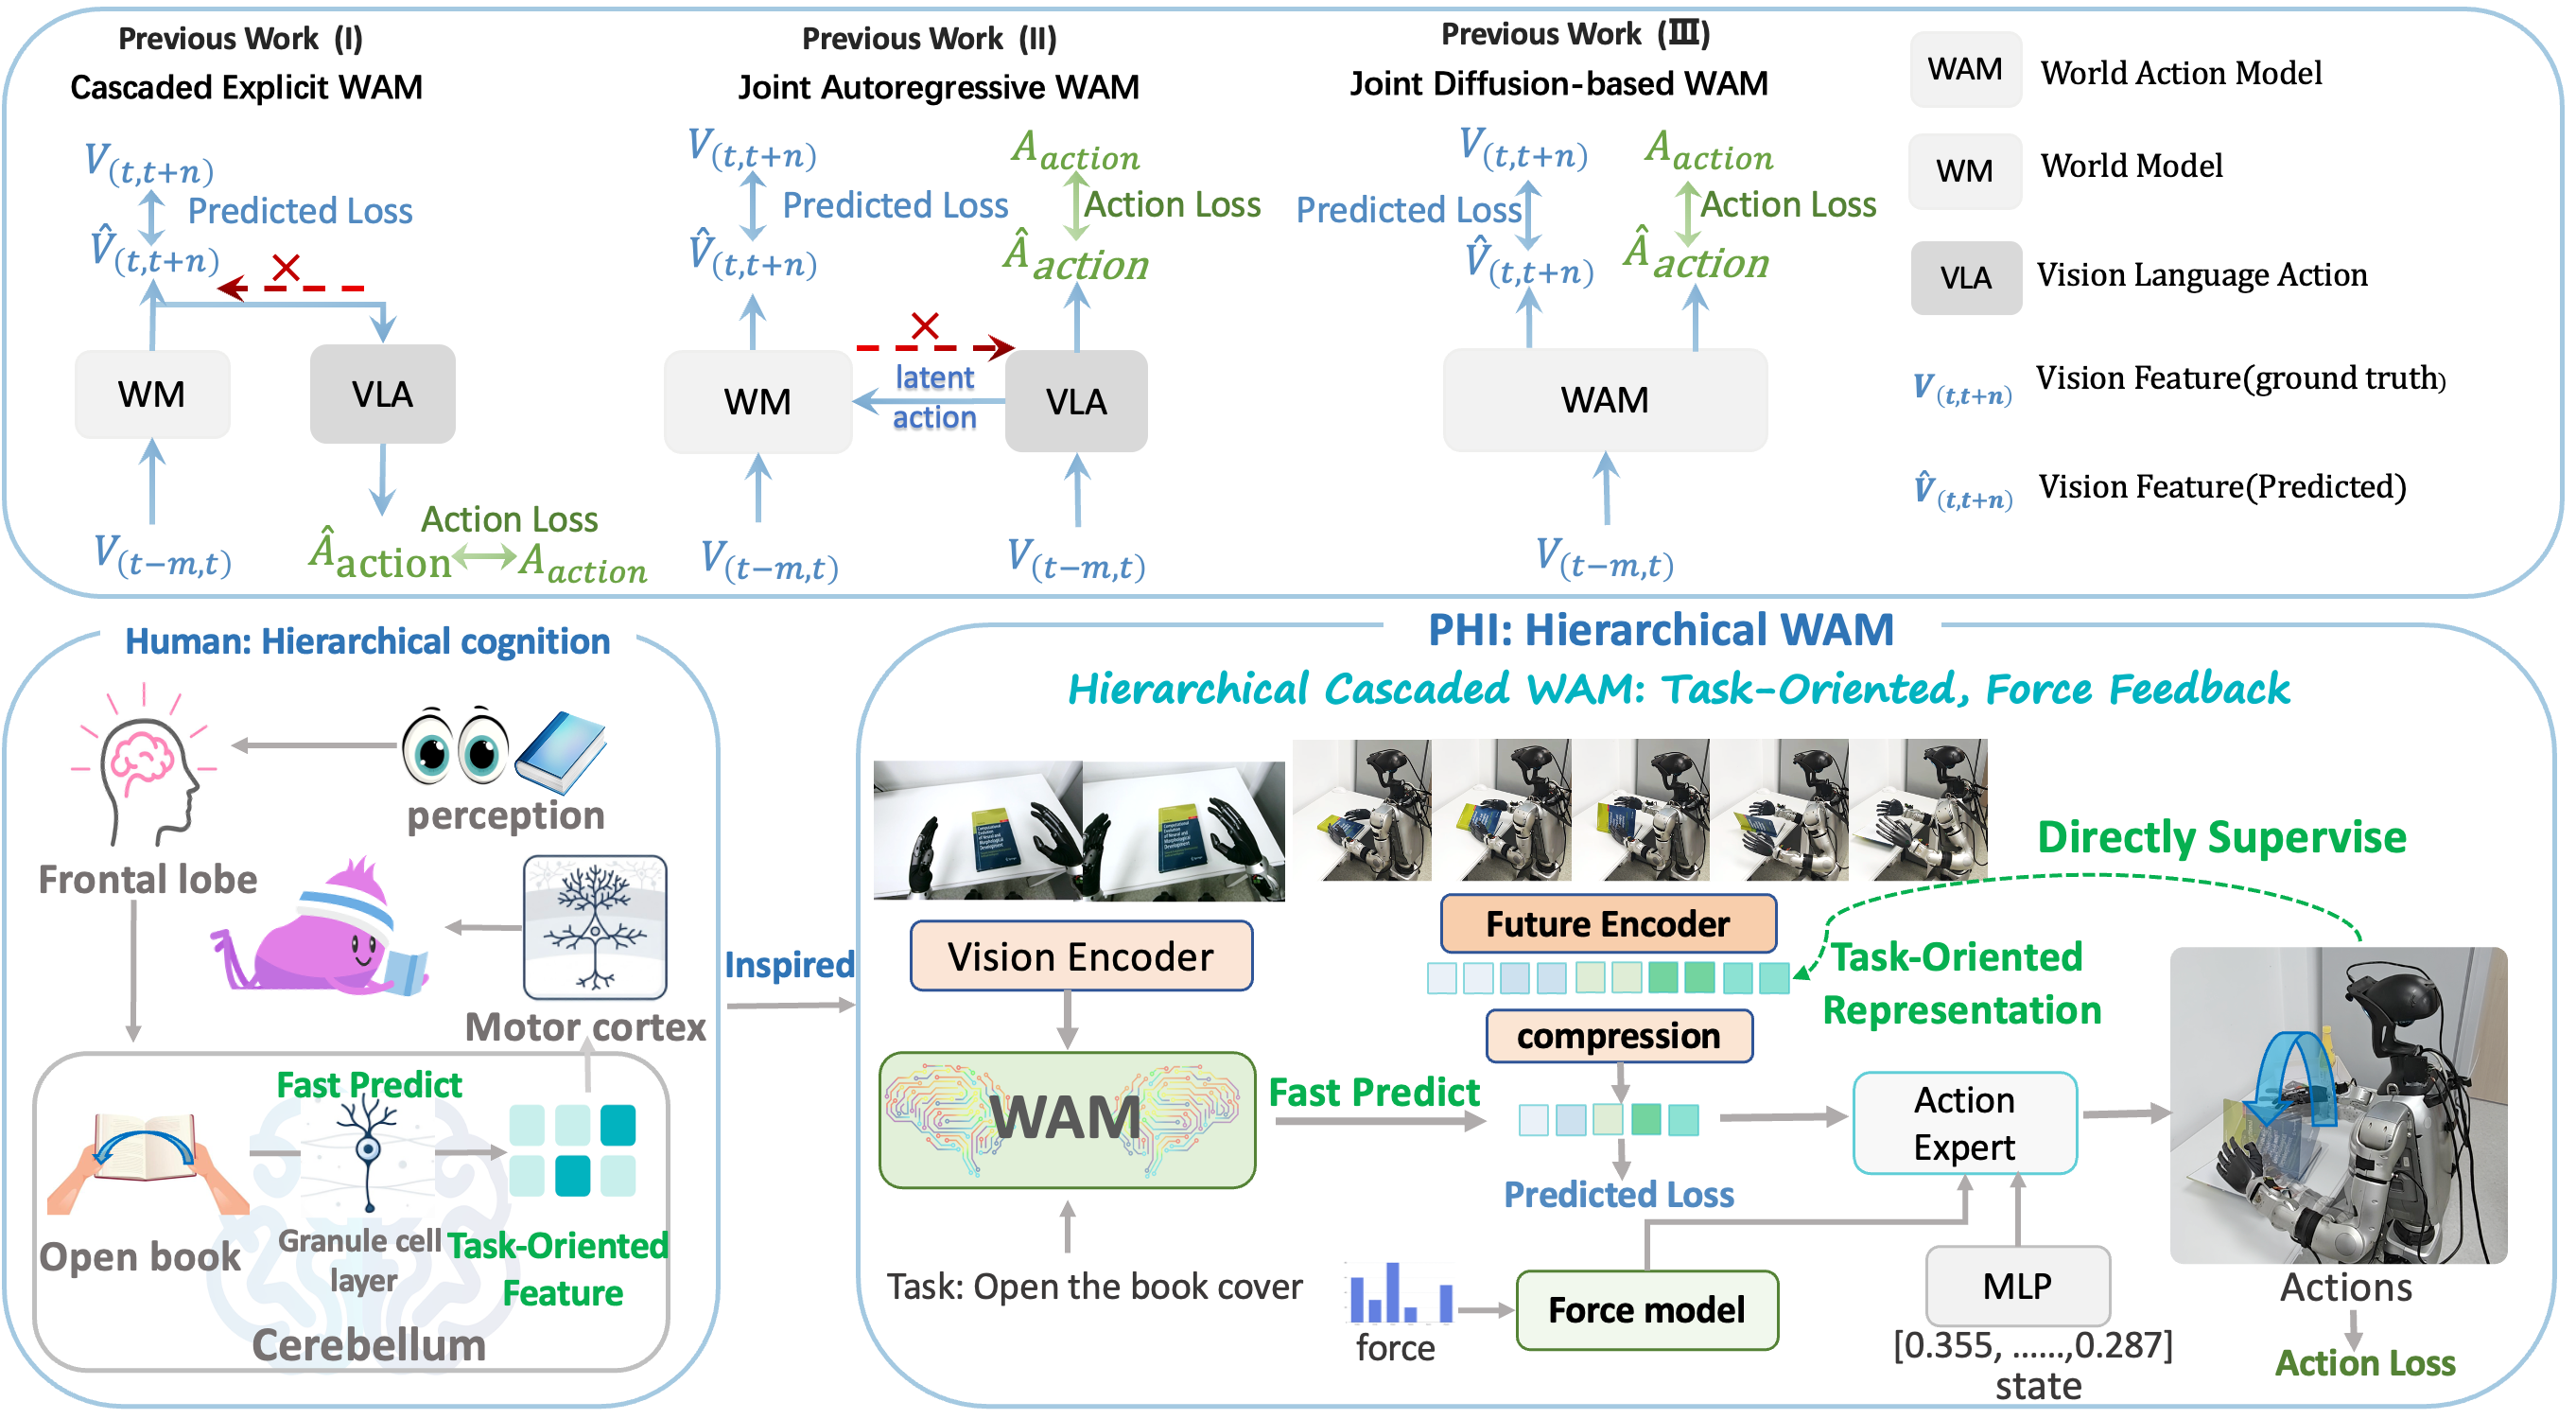
\includegraphics[width=\textwidth]{figures/head_image5.png}
\caption{Comparison of future representation learning paradigms. Existing approaches learn future visual representations through video prediction, with or without action conditioning, while PHI learns future representations grounded in their utility for downstream action generation.}
\label{headimage}
\end{figure}
% \section{Introduction}

% Complex bimanual manipulation requires robots to reason not only about the current state of the environment, but also about how objects and physical interactions will evolve during execution. This is particularly important for contact-rich tasks, where successful manipulation often depends on maintaining continuous contact, coordinating multiple degrees of freedom, and adapting actions to changing physical conditions. For example, turning a page or aligning a book requires the robot to anticipate future object configurations and contact transitions rather than reacting only to the current visual observation. Such tasks therefore call for manipulation policies that can explicitly reason about future interaction states.

% Recent vision-language-action (VLA) models have demonstrated strong generalization across a broad range of robotic manipulation tasks by directly mapping visual observations and language instructions to actions. However, these policies typically generate actions primarily from the current interaction context, providing limited explicit reasoning about how the environment will evolve after the current action. This limitation becomes particularly pronounced in long-horizon and contact-rich manipulation, where the appropriate action depends on future object states and interaction outcomes. Predictive world models offer a promising alternative by explicitly modeling future states and providing additional information for action generation and planning.

% Existing world-model approaches commonly learn future representations by optimizing predictive or reconstruction objectives. Pixel-space models predict future observations directly, while latent-space models learn compact representations of future states to improve prediction efficiency. Although these approaches can capture useful information about future observations, the objective of accurately predicting the future does not necessarily coincide with the objective of generating effective actions. A future representation may preserve visual details that are easy to predict but irrelevant to the downstream policy, while discarding task-specific information that is critical for action generation. In other words, \textbf{a representation that is effective for future prediction is not necessarily a representation that is useful for deciding what action to take}. This motivates a fundamental question: \textbf{can future visual representations be learned according to their downstream action utility, rather than prediction accuracy alone?}

% We argue that future representations should instead be grounded directly in the requirements of downstream manipulation. Rather than learning to reconstruct future observations as an end in itself, we learn future visual representations through their utility for action generation. Such action-grounded representations are encouraged to retain future information that is relevant to manipulation while avoiding unnecessary details that do not contribute to the policy. Once learned, these representations can serve as predictive targets for a VLA model, allowing the policy to infer action-relevant future states directly from the observed interaction context. This provides a more direct connection between future prediction and downstream control.

% However, visual information alone is insufficient to fully characterize contact-rich interactions. Physical interaction forces often contain information that is difficult to infer from vision, especially when contact states change subtly or when friction and force regulation determine the success of manipulation. Moreover, force signals evolve continuously over time, making their temporal dynamics important for distinguishing different interaction states. We therefore complement future visual representations with a temporal force representation that encodes recent force dynamics. The two modalities provide complementary information: the future visual representation captures \textbf{what the interaction is expected to look like}, while the temporal force representation captures \textbf{how the physical interaction is evolving}.

% Based on these observations, we propose \textbf{PHI (Predictive Hierarchical Intelligence)}, a predictive policy framework for contact-rich bimanual manipulation. PHI first learns future visual representations according to their downstream utility for action generation and then trains a VLA model to predict these action-grounded representations from the observed interaction context. In parallel, a temporal force module encodes recent force dynamics to capture physical interaction information that is difficult to obtain from vision alone. The predicted future visual representation and temporal force representation are subsequently combined to provide complementary guidance for action generation. Through this design, PHI connects future prediction directly to downstream control while explicitly incorporating the temporal evolution of physical interactions.

% We evaluate PHI on real-world manipulation tasks spanning different levels of interaction complexity, ranging from locomotion to contact-rich bimanual book manipulation. PHI consistently outperforms strong generalist VLA baselines, achieving a \textbf{20\% improvement in task success} and substantially stronger generalization to unseen books, with improvements reaching \textbf{30\%}. These results demonstrate that grounding future representations in downstream action utility, together with temporal modeling of force dynamics, provides an effective approach for robust and generalizable robotic manipulation.

% Our main contributions are summarized as follows:

% \begin{itemize}
%     \item We propose \textbf{PHI}, a predictive policy framework that learns action-grounded future visual representations and combines them with temporal force dynamics for contact-rich bimanual manipulation.
    
%     \item We introduce an action-grounded future representation learning paradigm that aligns future prediction with downstream action generation, and enable a VLA model to predict these representations from the observed interaction context.
    
%     \item We introduce a temporal force representation module that captures the evolution of physical interaction and provides complementary information to future visual representations for action generation.
    
%     \item We conduct extensive real-world experiments and demonstrate consistent improvements over strong VLA baselines, including a \textbf{20\% gain in task success} and up to \textbf{30\% improvement in generalization} to unseen books.
% \end{itemize}

\section{Introduction}

% Humanoid loco-manipulation is inherently sequential: choosing an action often requires reasoning not only about the current observation, but also about how object states and physical interactions are likely to evolve. This is particularly important in contact-rich bimanual manipulation, where successful execution depends on maintaining contact, coordinating multiple effectors, and transitioning between interaction phases as the physical state changes. For example, opening a book or aligning it on a table requires the robot to anticipate how the object and hand--object contacts may evolve, rather than reacting only to the current visual state. Such tasks therefore motivate policies that can exploit predictive information about the ongoing interaction when generating actions.

Humanoid bimanual dexterous manipulation requires coordinating dual-arm motions and fine-grained finger actions under continuously evolving physical interactions \cite{chen2024bidexhands,liu2025rdt}. This is particularly challenging in contact-rich tasks, where subtle changes in deformation, slip, separation, or contact mode can demand substantially different actions despite similar visual observations \cite{liu2025dextrack}. Since such interaction states are only partially observable from vision \cite{liu2025vtdexmanip}, successful Humanoid manipulation requires both estimating the current physical interaction and anticipating how task-relevant dynamics may evolve.

% Many generalist robot policies directly map the current interaction context to actions. Vision-Language-Action (VLA) models, like OpenVLA, Pi05~\cite{kim2024openvla, black2024pi0,black2025pi05} predict actions from visual observations, language instructions, and robot states~\cite{brohan2023rt2,octo2024,}. Recent World Action Models (WAMs) additionally model future observations or latent video~\cite{ye2026worldactionmodelszeroshot,cen2025worldvla,cheang2024gr2,bi2025motusunifiedlatentaction,motubrainteam2026motubrainadvancedworldaction}. However, explicit visual prediction may require modeling high-dimensional content irrelevant to control, while recent latent predictive approaches suggest that future-video generation is not always necessary~\cite{sun2026vlajepa,yuan2026fastwamworldactionmodels}. This motivates a fundamental question: \textbf{what future information actually needs to be predicted for action generation?}

% We hypothesize that predictive representations for control need not be observation-complete; instead, they should preserve future information that is useful for the current action decision. Thus, prediction fidelity and control utility need not coincide. Rather than defining future representations through reconstruction alone, we let downstream action generation determine what information should be retained. This perspective is conceptually related to predictive motor-control theories in neuroscience~\cite{nguyen2025cerebellar,gao2018cortico}, without attempting to model their biological circuitry.

% 最终修改版
Many generalist robot policies directly map the current interaction context to actions. Vision-Language-Action (VLA) models, such as OpenVLA~\cite{kim2024openvla} and $\pi_{0.5}$ \cite{black2024pi0,black2025pi05}, predict actions from visual observations, language instructions, and robot states \cite{brohan2023rt2,octo2024}. Recent World Action Models (WAMs), such as WorldVLA~\cite{cen2025worldvla} and GR-2~\cite{cheang2024gr2}, further incorporate future prediction into action-oriented modeling. Existing approaches predominantly learn to predict or reconstruct future visual observations, either explicitly at the image or video level~\cite{ye2026worldactionmodelszeroshot,motubrainteam2026motubrainadvancedworldaction} or implicitly in a latent space~\cite{cen2025worldvla,sun2026vlajepa}. While latent prediction avoids the cost of pixel-level reconstruction, the underlying predictive objective remains centered on representing the future observation~\cite{bi2025motusunifiedlatentaction}. This can lead the model to preserve visual information that is predictable but unnecessary for the current task~\cite{yuan2026fastwamworldactionmodels}, leaving an important question under-specified: \textbf{what information should a future representation preserve to support downstream action generation?}

We explore this question by shifting the focus from reconstructing future observations to learning task oriented future representations. Inspired by how the brain may selectively process and represent information according to ongoing goals~\cite{nguyen2025cerebellar,gao2018cortico}, our method allows task oriented supervision to directly shape the predicted future representation, encouraging the model to selectively retain information that supports the current task. This enables a more selective and efficient representation of the future, focusing predictive capacity on task oriented information rather than reconstructing future observations in their entirety.



% Based on this idea, we propose \textbf{PHI (Predictive Hierarchical Intelligence)}, a task-oriented latent WAM for humanoid bimanual dexterous manipulation, as illustrated in Fig.~\ref{headimage}. PHI uses future observations only as privileged supervision and learns predictive representations through an \textbf{Exploit--Predict--Align} procedure. \emph{Exploit} extracts action-relevant latent tokens from future observations; \emph{Predict} infers these tokens from the currently available interaction context; and \emph{Align} jointly adapts the predictive representation and action policy for control. At deployment, the privileged future-observation pathway is removed entirely. Because vision alone cannot fully characterize contact-rich interaction, PHI further incorporates a compact temporal representation of recent force evolution. The predicted future visual representation provides \emph{anticipatory} information, while force history summarizes the evolving \emph{current physical interaction}. Together with the current vision-language context and robot state, they condition a flow-matching action expert for continuous action-chunk generation.

% We evaluate PHI on a real Unitree G1 humanoid across five tasks spanning locomotion, object placement, sustained bimanual contact, and friction-regulated manipulation. PHI improves aggregate success from $58.7\%$ to $82.0\%$ over strong general-purpose VLA baselines. PHI also remains effective under visual clutter and on unseen books with different appearances and physical properties, improving success by up to $30.0$ percentage points over the strongest baseline. These results demonstrate that future observations can serve as effective privileged supervision for learning compact, action-relevant predictive representations without explicit future-video generation at deployment.

Based on this perspective, we introduce \textbf{PHI (Predictive Hierarchical Intelligence)}, a hierarchical World Action Model for humanoid bimanual dexterous manipulation. As illustrated in Fig.\ref{headimage}, existing WAMs can be broadly categorized into following paradigms. Cascaded approaches first reconstruct future visual observations and then derive representations for action generation, emphasizing future visual reconstruction while also capturing task-irrelevant visual information \cite{cheang2024gr2}. In contrast, joint autoregressive and diffusion approaches learn future representations together with action representations, enabling more efficient latent prediction while establishing an indirect connection between the learned representation and task execution~\cite{sun2026vlajepa,motubrainteam2026motubrainadvancedworldaction}. These paradigms provide complementary ways to connect future modeling with action generation. In contrast, the human brain provides a different perspective by forming compact predictive representations and selectively emphasizing task oriented information for motor control \cite{nguyen2025cerebellar,gao2018cortico}.


% These approaches provide different ways to connect future modeling with action generation, ranging from explicit future reconstruction to efficient latent prediction and joint future-action modeling. 
% Complementary to these computational paradigms, the human brain provides a different perspective on how predictive information may be organized for action. Predictive sensorimotor processing can form compact internal representations to support rapid motor control, while selectively emphasizing information relevant to the current goal \cite{nguyen2025cerebellar,gao2018cortico}. This suggests a hierarchical organization in which abstract, task-relevant future information is formed before being used for motor execution.

% Inspired by this principle, PHI combines the efficiency of latent future prediction with a hierarchical, task-oriented organization of the predictive pathway. PHI adopts a \emph{cascaded latent WAM} that combines efficient latent prediction with direct task-oriented supervision, learning future representations without reconstructing future images or videos at the pixel level. Through an \textbf{Exploit–Predict–Align} procedure, PHI extracts future latents from privileged observations, predicts them from the current interaction context, and shapes them with downstream action supervision. For real-world humanoid manipulation, visual prediction alone may remain insufficient to capture evolving physical interactions. PHI therefore further incorporates \textbf{temporal force feedback}, which encodes temporal force representations and provides complementary physical information about contact establishment, loading, and interaction changes. The predicted future representation and force feedback are jointly provided to the action expert to guide action generation. Inspired by the effector-specific organization of the human motor cortex \cite{gordon2023somato}, the action expert also adopts structured pathways for different body effectors, as detailed in Sec.\ref{sec:method}.  We evaluate PHI on a real Unitree G1 humanoid across five tasks, achieving $82.0\%$ aggregate success, compared with $58.7\%$ for strong general-purpose VLA baselines, and up to $30.0$ percentage points of improvement on unseen books. Our main contributions are summarized as follows: 


Inspired by this principle, PHI combines efficient latent prediction with a hierarchical cascaded WAM that selectively learns future features useful for downstream action generation. PHI avoids pixel-level reconstruction and, through an \textbf{Exploit–Predict–Align} procedure, extracts future latents from privileged observations, predicts them from the current interaction context, and aligns them with downstream action supervision. For humanoid manipulation, PHI further incorporates temporal force feedback to encode force features and complement visual prediction with physical information about contact and interaction changes. The predicted future representation and force feedback jointly guide the action expert, which adopts structured pathways for different body effectors inspired by their organization in the human motor cortex \cite{gordon2023somato} as detailed in Sec.\ref{sec:method}.  We evaluate PHI on a real Unitree G1 humanoid across five tasks, achieving $82.0\%$ aggregate success, compared with $58.7\%$ for strong general-purpose VLA baselines, and up to $30.0$ percentage points of improvement on unseen books. Our main contributions are summarized as follows: 


% PHI adopts a \emph{cascaded latent WAM} that combines efficient latent prediction with direct task-oriented supervision, learning future representations without reconstructing future images or videos at the pixel level. PHI uses future observations only as privileged supervision through an \textbf{Exploit–Predict–Align} procedure to extract task-relevant future latents from privileged observations, predict them from the current interaction context, and directly shape them with downstream action supervision. For real-world humanoid manipulation, where physical interactions are difficult to fully infer from vision alone, PHI further introduces a temporal force module to capture the evolution of contact forces and complement the predicted future representation with physical interaction information. We evaluate PHI on a real Unitree G1 humanoid across five tasks spanning locomotion, object placement, sustained bimanual contact, and friction-regulated manipulation. PHI improves aggregate success from $58.7\%$ to $82.0\%$ over strong general-purpose VLA baselines and remains effective under visual clutter and on unseen books with different appearances and physical properties, improving success by up to $30.0$ percentage points over the strongest baseline. Our main contributions are summarized as follows:


% \begin{itemize}
    % \item  We introduce an \textbf{action-grounded formulation of predictive future representation learning}, in which future observations serve as privileged supervision while the learned representation is shaped by downstream action generation to retain task-relevant future information, rather than to reconstruct or faithfully encode the complete future observation.

    % \item We propose \textbf{PHI} and an \textbf{Exploit--Predict--Align} learning procedure that operationalizes this formulation: it first extracts action-relevant future latents from privileged future observations, then learns to predict them using only the currently available interaction context, and finally jointly adapts the predictive representation and action policy for control.
    
    % \item To capture physical interaction dynamics that may be weakly observable from vision, PHI further incorporates a \textbf{temporal force representation} of recent contact evolution, complementing anticipatory future representations with information about how the current interaction has unfolded over time. 
    

% \end{itemize}


\begin{itemize}
% \item We introduce \textbf{PHI}, a task-oriented WAM for learning predictive future representations.

% \item We develop an \textbf{Exploit--Predict--Align} procedure to learn task-relevant future representations from privileged future observations.

% \item We introduce a \textbf{temporal force representation} to capture evolving physical interactions beyond visual observations.
\item We introduce \textbf{PHI}, a hierarchical WAM that integrates selective future prediction and temporal force feedback for humanoid bimanual manipulation.

\item We develop an \textbf{Exploit--Predict--Align} procedure to learn task oriented future representations from privileged future observations and align them with downstream policy.

\item We introduce \textbf{temporal force feedback} to capture evolving physical interactions beyond visual observations and guide robust humanoid manipulation.
\end{itemize}




\section{Related Work}

\subsection{Future Modeling for Robot Action Generation}
\label{sec:related_future_prediction}

% Generalist vision-language-action policies learn to generate robot actions directly from visual observations, language instructions, and robot states. RT-2 transfers vision-language knowledge to robotic control~\cite{brohan2023rt2}, while Octo and OpenVLA further develop general-purpose robot policies through large-scale multimodal pretraining and robot demonstrations~\cite{octo2024,kim2024openvla}. More recently, $\pi_0$ combines a pretrained vision-language backbone with a flow-matching action expert for continuous control, and $\pi_{0.5}$ extends this paradigm through heterogeneous co-training across robots, tasks, and data sources~\cite{black2024pi0,black2025pi05}. These models provide strong policy backbones, but their action-generation pathways do not explicitly expose a predicted future interaction representation. World models provide an alternative mechanism for incorporating foresight into robot control. Classical latent world models learn compact dynamics for planning and control directly from observations~\cite{hafner2019planet,hafner2023dreamerv3,hansen2024tdmpc2}. In robotic manipulation, one line of work models future interaction explicitly in observation space. GR-1, UniPi, and RoboDreamer use future visual prediction or video generation to support robot policy learning and planning~\cite{wu2023gr1,du2023unipi,zhou2024robodreamer}. More recent World Action Models connect future modeling more tightly with action generation. WorldVLA autoregressively models future visual observations together with robot actions~\cite{cen2025worldvla}, while GR-2 combines generative video modeling with action prediction~\cite{cheang2024gr2}. Motus and MotuBrain further explore unified latent-action or world-action formulations for robot control~\cite{bi2025motusunifiedlatentaction,motubrainteam2026motubrainadvancedworldaction}. These developments have led to a broader WAM paradigm in which representations of future world evolution are integrated with action prediction~\cite{ye2026worldactionmodelszeroshot}. Fast-WAM further shows that future-video modeling can be useful during training even when explicit future imagination is removed from the inference pathway~\cite{yuan2026fastwamworldactionmodels}.

% A complementary direction avoids explicit future-image reconstruction and instead models temporal structure in latent space. Latent Action Pretraining (LAPA) learns latent actions from videos, while Moto uses latent motion tokens as an intermediate representation for robot manipulation~\cite{ye2024lapa,chen2024moto}. VLA-JEPA directly predicts latent representations of future observations through predictive alignment, demonstrating that future information can be incorporated into VLA policies without reconstructing future pixels~\cite{sun2026vlajepa}. These approaches establish the value of compact latent prediction. PHI focuses on a complementary design question: \emph{how should the target future representation itself be defined?} Rather than treating the future latent as a representation specified primarily by reconstruction, transition modeling, or representation matching, PHI first allows downstream action generation to shape the information retained by the privileged future latent. The resulting action-grounded representation is then used as the prediction target for a causal model operating only on the current interaction context. In this sense, PHI shifts the emphasis from predicting a complete or predefined future representation toward learning a compact future representation whose content is selected according to downstream control utility.
% Generalist vision-language-action policies generate robot actions from
% visual observations, language instructions, and robot states. RT-2 transfers
% vision-language knowledge to robotic control~\cite{brohan2023rt2}, while Octo
% and OpenVLA develop general-purpose policies through large-scale multimodal
% pretraining and robot demonstrations~\cite{octo2024,kim2024openvla}. More
% recently, $\pi_0$ combines a pretrained vision-language backbone with a
% flow-matching action expert, and $\pi_{0.5}$ extends this paradigm through
% heterogeneous co-training across robots, tasks, and data sources
% ~\cite{black2024pi0,black2025pi05}. While these models provide strong policy
% backbones, their action-generation pathways do not explicitly expose a
% predicted future interaction representation. World models provide an alternative way to incorporate foresight into robot
% control. Classical latent world models learn compact dynamics for planning
% and control~\cite{hafner2019planet,hafner2023dreamerv3,hansen2024tdmpc2},
% while robotic manipulation methods such as GR-1, UniPi, and RoboDreamer
% model future interaction through visual prediction or video generation
% ~\cite{wu2023gr1,du2023unipi,zhou2024robodreamer}. More recent World Action
% Models connect future modeling directly with action generation: WorldVLA
% models future visual observations together with robot actions, while GR-2
% combines generative video modeling with action prediction
% ~\cite{cen2025worldvla,cheang2024gr2}. Motus and MotuBrain further explore
% unified latent-action or world-action formulations, contributing to the
% broader WAM paradigm~\cite{bi2025motusunifiedlatentaction,motubrainteam2026motubrainadvancedworldaction,ye2026worldactionmodelszeroshot}.
% Fast-WAM further shows that future-video modeling can be useful during
% training even when explicit future imagination is removed at inference
% ~\cite{yuan2026fastwamworldactionmodels}. A complementary direction predicts future structure directly in latent
% space. LAPA learns latent actions from videos, Moto uses latent motion
% tokens for manipulation, and VLA-JEPA predicts future latent
% representations without reconstructing future pixels
% ~\cite{ye2024lapa,chen2024moto,sun2026vlajepa}. These works demonstrate
% the value of compact latent prediction. PHI instead focuses on how the
% future target should be defined: rather than specifying the target through future-image reconstruction, transition modeling, or representation matching alone, PHI lets downstream action generation shape the privileged future latent. This action-grounded representation is then used
% as the target for a causal predictor that operates only on the current
% interaction context.


Generalist vision-language-action policies generate robot actions from visual observations, language instructions, and robot states. RT-2 transfers vision-language knowledge to robotic control~\cite{brohan2023rt2}, while Octo and OpenVLA develop general-purpose policies through large-scale multimodal pretraining and robot demonstrations~\cite{octo2024,kim2024openvla}. $\pi_0$ combines a pretrained vision-language backbone with a flow-matching action expert, while $\pi_{0.5}$ extends this paradigm through heterogeneous co-training across robots, tasks, and data sources~\cite{black2024pi0,black2025pi05}. While these models provide strong policy backbones, they do not explicitly model future interaction representations. World models provide an alternative way to incorporate foresight into robot control. Classical latent world models learn compact dynamics for planning and control~\cite{hafner2019planet,hafner2023dreamerv3,hansen2024tdmpc2}, while robotic manipulation methods such as GR-1, UniPi, and RoboDreamer model future interactions through visual prediction or video generation~\cite{wu2023gr1,du2023unipi,zhou2024robodreamer}. More recent World Action Models (WAMs) connect future modeling with action generation: WorldVLA models future visual observations with robot actions~\cite{cen2025worldvla}, while GR-2 combines video generation with action prediction~\cite{cheang2024gr2}. Motus and MotuBrain further explore unified latent action and world action formulations~\cite{bi2025motusunifiedlatentaction,motubrainteam2026motubrainadvancedworldaction}, while Fast-WAM uses future-video modeling as training supervision without explicit future prediction at inference~\cite{yuan2026fastwamworldactionmodels}. In latent space, LAPA learns latent actions, Moto predicts latent motion tokens, and VLA-JEPA predicts future representations without pixel reconstruction~\cite{ye2024lapa,chen2024moto,sun2026vlajepa}. PHI instead learns \emph{task-oriented future representations}, using downstream action supervision to shape the privileged future latent, which is then predicted from the current context for action generation.

% More recent World Action Models (WAMs) connect future modeling with action generation: WorldVLA models future visual observations together with robot actions, while GR-2 combines generative video modeling with action prediction~\cite{cen2025worldvla,cheang2024gr2}. Motus and MotuBrain further explore unified latent-action and world-action formulations~\cite{bi2025motusunifiedlatentaction,motubrainteam2026motubrainadvancedworldaction,ye2026worldactionmodelszeroshot}. Fast-WAM shows that future-video modeling can provide useful training supervision even when explicit future prediction is removed at inference~\cite{yuan2026fastwamworldactionmodels}. Another line of work predicts future structure directly in latent space. LAPA learns latent actions from videos, Moto uses latent motion tokens for manipulation, and VLA-JEPA predicts future latent representations without reconstructing future pixels~\cite{ye2024lapa,chen2024moto,sun2026vlajepa}. These works demonstrate the efficiency of compact latent prediction. PHI instead focuses on learning \emph{task-oriented future representations}: rather than defining the future target through image reconstruction, transition modeling, or representation matching alone, PHI uses downstream action supervision to shape the privileged future latent. The resulting representation is then predicted from the current interaction context and used for task-oriented action generation.

% \subsection{Force-Aware Contact-Rich Manipulation}
% \label{sec:related_force_aware}

% Vision alone provides incomplete information about many contact-rich interactions. Changes in contact establishment, friction, loading, and interaction force may correspond to only small visual changes, motivating the integration of force and tactile sensing into learning-based manipulation policies. ForceMimic jointly models time-varying force and motion for contact-rich imitation learning~\cite{liu2025forcemimic}, while FoAR uses visual observations together with high-frequency force/torque sensing and future contact prediction for force-aware reactive control~\cite{he2024foar}. Reactive Diffusion Policy (RDP) similarly combines a slower visual action pathway with fast tactile feedback to improve responsiveness during physical interaction~\cite{xue2025rdp}.

% Force sensing has also been incorporated into generalist VLA architectures. ForceVLA extends $\pi_0$ with a force-aware mixture-of-experts module that conditions action decoding on real-time force measurements~\cite{yu2025forcevla}. ForceVLA2 incorporates force-aware task representations and real-time force feedback for hybrid force-position control~\cite{li2026forcevla2}, while TaF-VLA aligns tactile observations with physical force measurements before integrating the resulting representation into a VLA backbone~\cite{huang2026tafvla}. FAVLA adopts a force-adaptive slow--fast architecture that combines near-future force prediction with high-frequency force observations for reactive manipulation~\cite{li2026favla}. These approaches demonstrate the value of physical sensing for multimodal policy conditioning and force regulation.

% A closely related direction explicitly models the temporal structure of force signals. FM-VLA compresses force histories into memory tokens and uses them to provide non-Markovian physical context to the action policy~\cite{li2026fmvla}. PHI also exploits force history, but uses it in a different role within the predictive architecture. Rather than reconstructing dense tactile observations, maintaining long-term force-event memory, or explicitly predicting future force targets, PHI encodes a short history of low-dimensional force measurements into a compact representation of \emph{ongoing physical interaction}. This representation complements the predicted future visual latent: the former summarizes recent contact evolution, while the latter provides anticipatory information about likely task evolution. Their combination provides the action expert with complementary physical and predictive context for contact-rich manipulation.

\subsection{Force-Aware Manipulation}
\label{sec:related_force_aware}

Vision alone provides incomplete information for contact-rich manipulation,
motivating the integration of force and tactile sensing into learning-based
policies. Existing methods incorporate physical sensing in different ways:
ForceMimic jointly models time-varying force and motion for contact-rich
imitation learning~\cite{liu2025forcemimic}, while FoAR and Reactive
Diffusion Policy (RDP) combine visual observations with force or tactile
feedback for reactive control~\cite{he2024foar,xue2025rdp}. Recent VLA-based
approaches further integrate physical sensing into generalist policies,
including force-aware action decoding~\cite{yu2025forcevla}, force-aware task
representations and hybrid force-position control~\cite{li2026forcevla2},
tactile-force alignment~\cite{huang2026tafvla}, and slow fast force
adaptation~\cite{li2026favla}. These studies highlight the benefits of
physical sensing for multimodal action generation and force regulation. A related line of work models the temporal structure of force signals.
FM-VLA compresses force histories into memory tokens to provide
non-Markovian physical context~\cite{li2026fmvla}. PHI instead uses a short
history of low-dimensional force measurements to encode the \emph{ongoing
physical interaction}, complementing the predicted future visual latent.
The force representation captures recent contact evolution, while the
future latent provides anticipatory information about task evolution,
together supplying complementary physical and predictive context for
contact-rich action generation.

% \section{Related Work}

% \subsection{Future Prediction for Manipulation}
% \label{sec:related_future_prediction}

% Recent vision-language-action (VLA) models have demonstrated strong
% generalization across diverse robotic manipulation tasks by leveraging
% large-scale vision-language pretraining and robot demonstrations
% \cite{brohan2023rt2,octo2024,kim2024openvla}.
% Recent generalist policies such as $\pi_0$ and $\pi_{0.5}$ further
% improve manipulation capabilities by combining pretrained
% vision-language models with action experts and heterogeneous training
% data \cite{black2024pi0,black2025pi05}.
% In particular, $\pi_{0.5}$ extends the VLA paradigm toward more
% generalizable and long-horizon manipulation through large-scale
% co-training across diverse robot and non-robot data
% \cite{black2025pi05}.
% Despite their strong performance, these policies primarily generate
% actions from current observations and task instructions, without
% explicitly representing how the environment may evolve in the future.

% To provide additional guidance for long-horizon manipulation, recent
% works explore predicting future observations or future states.
% Pixel-level world models explicitly predict future images or videos,
% providing rich visual foresight for planning and control
% \cite{wu2023gr1,du2023unipi,zhou2024robodreamer}.
% While such approaches preserve detailed information about future
% observations, modeling high-dimensional pixel spaces can be
% computationally expensive and may require the model to capture
% appearance changes that are not directly relevant to action generation.
% An alternative line of work therefore performs future prediction in
% latent spaces, learning compact representations of future states or
% transitions
% \cite{hafner2019planet,hafner2023dreamerv3,hansen2024tdmpc2}.
% Recent VLA approaches further explore latent future embeddings and
% latent actions to leverage large-scale video data and learn temporal
% representations without explicitly reconstructing future observations
% \cite{ye2024lapa,chen2024moto,sun2026vlajepa}.
% For example, VLA-JEPA predicts future latent representations through
% predictive alignment, encouraging the model to capture action-relevant
% dynamics while avoiding explicit pixel-level reconstruction and
% future-information leakage \cite{sun2026vlajepa}.

% While latent prediction provides a more efficient alternative to
% pixel-level future modeling, existing approaches mainly learn future
% representations through reconstruction, predictive alignment, or
% frame-transition objectives
% \cite{hafner2019planet,ye2024lapa,chen2024moto,sun2026vlajepa}.
% Such objectives do not necessarily ensure that the predicted future
% representations are optimized for how a downstream manipulation policy
% actually uses future information.
% In contrast, PHI progressively aligns future latent learning with
% policy generation.
% Specifically, PHI first trains the policy to exploit privileged future
% information extracted from future observations, then distills this
% information into future latent tokens predicted from current
% observations, and finally jointly optimizes the latent predictor and
% action expert to align future prediction with downstream action
% generation.
% This progressive design enables future latent representations to serve
% as explicit planning signals while retaining the efficiency of
% latent-space prediction.

% \subsection{Force-Aware Manipulation}
% \label{sec:related_force_aware}

% Contact-rich manipulation requires policies to reason about physical
% interactions that are only partially observable from vision, such as
% contact establishment, interaction strength, and evolving contact
% dynamics.
% Force and tactile sensing have therefore been incorporated into
% learning-based manipulation policies to provide complementary physical
% feedback.
% ForceMimic introduces a force-centric imitation learning framework that
% jointly models time-varying force and motion for contact-rich
% manipulation \cite{liu2025forcemimic}, while FoAR combines visual
% observations with high-frequency force/torque sensing and uses a future
% contact predictor to adapt the use of force feedback across different
% contact phases \cite{he2024foar}.
% Reactive Diffusion Policy (RDP) further introduces a slow--fast
% visual-tactile policy, using a slow latent diffusion policy to generate
% high-level action chunks and a fast tactile-feedback policy for reactive
% contact control \cite{xue2025rdp}.

% Recent work has also incorporated force sensing into generalist
% vision-language-action (VLA) models.
% ForceVLA extends the $\pi_0$ framework with a force-aware
% mixture-of-experts module that fuses visual-language representations
% with real-time 6-axis force feedback during action decoding
% \cite{yu2025forcevla}.
% ForceVLA2 further incorporates force-aware task concepts into the VLM
% and combines them with real-time force feedback in the action expert for
% hybrid force-position control \cite{li2026forcevla2}.
% In parallel, TaF-VLA aligns high-dimensional tactile observations with
% physical force measurements and integrates the resulting force-aware
% tactile representation into a VLA backbone
% \cite{huang2026tafvla}.
% FAVLA adopts a force-adaptive slow--fast VLA architecture, in which a
% slow VLM predicts near-future force variation and a fast action expert
% uses high-frequency force sequences for reactive control
% \cite{li2026favla}.
% These approaches demonstrate the importance of physical sensing for
% contact-rich manipulation, but primarily focus on multimodal fusion,
% force-aware task representation, tactile-force alignment, or explicit
% force regulation.

% A closely related direction is to exploit the temporal evolution of
% force signals rather than relying only on instantaneous measurements.
% FM-VLA introduces force-based memory for VLA models by encoding force
% histories into compact memory tokens and conditioning the action expert
% on the resulting temporal representation \cite{li2026fmvla}.
% Specifically, its force memory is pretrained using force time-series
% reconstruction and is designed to retain past contact events for
% non-Markovian manipulation tasks.
% This demonstrates that historical force signals can provide useful
% information about past physical interactions that may be ambiguous from
% the current visual observation.

% In contrast, our goal is to capture the continuous evolution of
% low-dimensional force signals as a compact representation of ongoing
% contact dynamics.
% Rather than reconstructing dense tactile observations, learning a
% long-term force-event memory, or explicitly predicting future force
% targets, PHI directly encodes a short force history with a temporal
% network and provides the resulting force representation as a dedicated
% condition to the action expert.
% Together with the predicted future visual latent, this enables the
% policy to jointly exploit anticipated visual information and evolving
% physical feedback for contact-rich manipulation.


% \section{Method}

% \begin{figure}[th]
% \centering
% 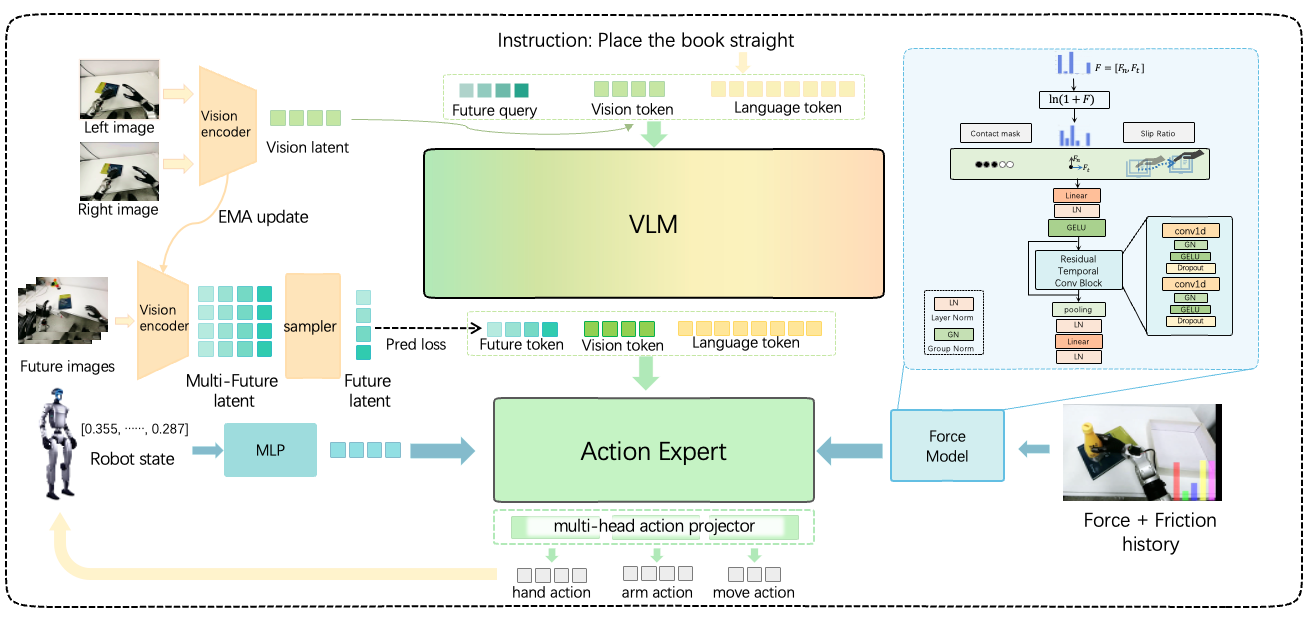
\includegraphics[width=\textwidth]{figures/frame.png}
% \caption{Architecture Framework.}
% \end{figure}

% \subsection{Problem Formulation and Overview}

% We consider the problem of learning a policy for complex bimanual
% manipulation from multimodal demonstrations. At each time step $t$, the robot
% receives a visual observation $I_t$, a language instruction $\ell$, the
% robot proprioceptive state $s_t$, and a history of force measurements
% $F_{t-K+1:t}$. The policy predicts an action chunk
% $A_t = [a_t,\ldots,a_{t+H-1}]$ through a flow-matching action expert. Formally,
% our policy can be written as
% \begin{equation}
%     A_t \sim
%     \pi_{\theta}
%     \left(
%         A_t \mid
%         I_t,\ell,s_t,F_{t-K+1:t}
%     \right),
% \end{equation}
% where $K$ denotes the length of the force history and $H$ denotes the action
% chunk horizon.

% Our framework, \textbf{PHI}, is built upon a vision-language-action policy
% with a vision-language model (VLM) and a flow-matching action expert. While
% the VLM provides rich semantic and visual context, visual observations alone
% may not fully reveal the physical state of an ongoing interaction. In
% particular, contact establishment, interaction strength, and changes in
% physical interaction can evolve continuously while producing only subtle
% visual changes. We therefore introduce a temporal force perception module
% that encodes the recent history of low-dimensional force measurements into a
% compact physical-interaction representation.

% In addition, conditioning action generation only on the current observation
% can lead to myopic decision making for long-horizon manipulation. PHI
% therefore augments the policy with a predictive future visual
% representation. During training, future observations are encoded into a
% compact latent representation that is learned through the downstream action
% generation objective. The VLM is subsequently trained to predict this
% future representation from the current observation and language instruction,
% allowing the policy to obtain anticipatory information without accessing
% future observations at inference time.

%     As illustrated in Fig.~\ref{fig:overview}, PHI therefore combines two
% complementary sources of information for action generation:
% \emph{temporal physical feedback} from force history and
% \emph{predictive visual information} from future latent representations.
% The resulting representations are provided to the flow-matching action
% expert, which generates the final action chunk. Importantly, future
% observations are used only as privileged supervision during training and are
% fully removed during inference.

% \subsection{PHI: Force-Aware Predictive Policy}

% \subsubsection{Temporal Force Perception}

% Unlike dense tactile observations that provide spatially detailed information
% about contact surfaces, our force measurements are low-dimensional and
% provide limited spatial information. We therefore focus on a complementary
% property of force sensing: its continuous temporal evolution. Changes in
% force magnitude and the relationship between normal and tangential forces
% provide useful cues about evolving contact states and physical interaction
% dynamics that may not be directly observable from a single image.

% Given the recent force history
% $F_{t-K+1:t} \in \mathbb{R}^{K \times d_f}$, we first construct a
% contact-aware representation through a lightweight feature transformation
% $\phi(\cdot)$. Specifically, in addition to the raw force measurements, we
% derive force magnitudes on a logarithmic scale, binary contact indicators,
% and tangential-to-normal force ratios. The resulting sequence is given by
% \begin{equation}
%     \widetilde{F}_{t-K+1:t}
%     =
%     \phi(F_{t-K+1:t}).
% \end{equation}

% We then employ a temporal encoder $E_f$ based on dilated temporal
% convolutions to aggregate information across the force history:
% \begin{equation}
%     z_t^f
%     =
%     E_f
%     \left(
%         \widetilde{F}_{t-K+1:t}
%     \right),
% \end{equation}
% where $z_t^f$ denotes the resulting force representation. The dilated
% temporal convolutions allow the encoder to capture force variations over
% multiple temporal scales while maintaining a compact representation. Unlike
% methods that treat force as an instantaneous state variable, our force
% encoder explicitly models the evolution of physical interaction over time.

% The resulting representation is projected into the feature space of the
% action expert and represented as a dedicated force token. This force token
% is used only for action generation and does not participate in predicting the
% future visual representation. Consequently, the force pathway provides
% complementary information about the current physical interaction without
% introducing future information into the predictive pathway.

% \subsubsection{Future Latent Representation}

% To provide the policy with information about the consequences of ongoing
% interaction, we introduce a predictive representation of future visual
% observations. Rather than reconstructing future images at the pixel level,
% we represent future observations in a compact latent space that is more
% closely coupled to downstream action generation.

% For each training sample, we select $M$ future observation times
% $t+\Delta_1,\ldots,t+\Delta_M$. A vision encoder $E_v$ first extracts visual
% features from the corresponding future observations. The resulting features
% are aggregated by a Perceiver-based resampler $R_\psi$ to obtain a fixed
% number of future latent tokens:
% \begin{equation}
%     Z_t^{+}
%     =
%     R_\psi
%     \left(
%         E_v(I_{t+\Delta_1}),
%         \ldots,
%         E_v(I_{t+\Delta_M})
%     \right),
% \end{equation}
% where $Z_t^{+}$ denotes the target future representation.

% A key design choice is that the future representation is not learned through
% a future-image reconstruction objective. Instead, during the first training
% stage, the future representation extractor is optimized through the
% downstream action generation objective. Consequently, $Z_t^{+}$ is encouraged
% to retain information that is useful for predicting future actions rather
% than merely encoding pixel-level appearance changes.

% To remove the dependence on future observations at inference time, PHI
% introduces a set of learnable future query tokens into the VLM. Given the
% current visual observation and language instruction, the VLM predicts the
% corresponding future representation:
% \begin{equation}
%     \widehat{Z}_t^{+}
%     =
%     P_\theta(I_t,\ell),
% \end{equation}
% where $P_\theta$ denotes the future prediction pathway of the VLM. During
% training, $\widehat{Z}_t^{+}$ is supervised using the action-grounded target
% representation $Z_t^{+}$. At inference time, only
% $\widehat{Z}_t^{+}$ is available, while the future observation encoder and
% the target representation pathway are discarded.

% \subsubsection{Force- and Future-Conditioned Action Generation}

% PHI combines the predicted future representation with temporal force
% information within the action generation process. The VLM first processes
% the current visual observation and language instruction to produce a
% vision-language representation $Z_t^{vl}$ together with the predicted
% future latent tokens $\widehat{Z}_t^{+}$. In parallel, the force encoder
% produces the temporal force token $z_t^f$, while the robot state is projected
% into a state representation $z_t^s$.

% These representations are provided to the flow-matching action expert,
% which generates an action chunk conditioned on both anticipated visual
% information and current physical interaction:
% \begin{equation}
%     v_\theta
%     =
%     G_\theta
%     \left(
%         A_t^\tau,
%         Z_t^{vl},
%         \widehat{Z}_t^{+},
%         z_t^f,
%         z_t^s
%     \right),
% \end{equation}
% where $A_t^\tau$ denotes an intermediate noisy action trajectory along the
% flow-matching path and $v_\theta$ is the predicted velocity field. The final
% action chunk is obtained by integrating the learned flow from the noise
% distribution toward the demonstrated action distribution.

% The predicted future latent and temporal force representation play
% complementary roles in this process. The future latent provides
% \emph{anticipatory visual context}, helping the policy reason about the
% potential future state of the manipulation, whereas the force representation
% provides \emph{temporal physical context}, describing how the current
% interaction is evolving. Their combination allows the action expert to
% generate actions using both predicted future information and continuously
% observed physical feedback.

% For the large action space of our bimanual robot, PHI further decomposes
% action generation into multiple body-part-specific projection heads. Each
% projector maps the shared action-expert representation into the action space
% of a corresponding body part, enabling the policy to model heterogeneous
% motion dimensions while maintaining a shared multimodal representation.
% This design is particularly important for complex bimanual manipulation,
% where the action space involves coordinated motions across multiple body
% parts rather than a single compact end-effector action.

% \subsection{Progressive Future-Latent Learning}

% The future representation introduced in Sec.~3.2 provides useful
% anticipatory information for action generation, but directly learning such a
% representation from current observations is challenging. In particular, the
% future representation should not merely encode visually predictable changes;
% it should capture information that is useful for downstream action
% generation. At the same time, directly optimizing the VLM to predict such a
% representation while simultaneously learning the action policy introduces
% two coupled learning problems: the future representation itself is still
% evolving, while the policy must learn to exploit it.

% To address this challenge, we introduce a progressive three-stage training
% strategy. The key idea is to first learn an \emph{action-grounded future
% representation} using privileged future observations, then teach the VLM to
% predict this representation from the current observation, and finally
% jointly optimize the VLM and action expert to align the predicted future
% representation with downstream action generation. The three stages
% correspond to \emph{exploit}, \emph{predict}, and \emph{align}, respectively.
% This progressive design separates representation discovery from future
% prediction and policy optimization, leading to a more stable learning
% process.

% \subsubsection{Learning to Exploit Future Information}

% In the first stage, we provide the policy with the target future
% representation $Z_t^{+}$ obtained from future observations. The purpose of
% this stage is not to teach the VLM to predict the future, but to learn what
% future information is useful for action generation.

% Specifically, the target future representation is extracted as
% \begin{equation}
%     Z_t^{+}
%     =
%     R_{\psi}
%     \left(
%         E_v(I_{t+\Delta_1}),
%         \ldots,
%         E_v(I_{t+\Delta_M})
%     \right),
% \end{equation}
% and is directly provided to the action expert together with the current
% vision-language representation, force representation, and robot state:
% \begin{equation}
%     v_{\theta}
%     =
%     G_{\theta}
%     \left(
%         A_t^\tau,
%         Z_t^{vl},
%         Z_t^{+},
%         z_t^f,
%         z_t^s
%     \right).
% \end{equation}

% The parameters of the future representation pathway and the action expert
% are optimized according to the downstream action objective. In this way,
% the future representation is learned in an action-grounded manner: the
% representation is encouraged to preserve information that helps distinguish
% different future states that are relevant for generating the demonstrated
% actions, rather than information that is only useful for reconstructing
% future visual appearances.

% For flow matching, we construct an interpolation between a sampled noise
% trajectory $A_t^0$ and the demonstrated action chunk $A_t^1$:
% \begin{equation}
%     A_t^\tau
%     =
%     (1-\tau)A_t^0 + \tau A_t^1,
%     \qquad
%     \tau \sim \mathcal{U}(0,1),
% \end{equation}
% with the corresponding target velocity
% \begin{equation}
%     u_t
%     =
%     A_t^1-A_t^0.
% \end{equation}
% The action objective is therefore
% \begin{equation}
%     \mathcal{L}_{\mathrm{action}}
%     =
%     \mathbb{E}_{\tau,A_t^0,A_t^1}
%     \left[
%         \left\|
%         v_{\theta}
%         \left(
%             A_t^\tau,
%             Z_t^{vl},
%             Z_t^{+},
%             z_t^f,
%             z_t^s
%         \right)
%         -
%         u_t
%         \right\|_2^2
%     \right].
% \end{equation}

% Thus, Stage I establishes an action-grounded target space for future
% information before asking the VLM to predict it. This privileged training
% signal is particularly important because the target future representation
% is not defined by pixel-level reconstruction, but by its utility for
% downstream manipulation.

% \subsubsection{Learning to Predict Future Information}

% After the future representation has been grounded by the action-generation
% objective, the second stage transfers the ability to obtain future
% information from privileged observations to the current observation.

% During this stage, the target future representation $Z_t^{+}$ is treated as
% a fixed supervision target. We freeze the future representation pathway and
% the action expert, and optimize the VLM to predict the target representation
% using only the current observation and language instruction. Specifically,
% the future query tokens introduced in Sec.~3.2 are appended to the VLM
% output sequence, producing
% \begin{equation}
%     \widehat{Z}_t^{+}
%     =
%     P_{\theta}(I_t,\ell).
% \end{equation}

% We supervise the predicted representation against the target representation
% using a latent alignment objective:
% \begin{equation}
%     \mathcal{L}_{\mathrm{future}}
%     =
%     \left\|
%         \widehat{Z}_t^{+}
%         -
%         \operatorname{sg}
%         \left(
%             Z_t^{+}
%         \right)
%     \right\|_2^2,
% \end{equation}
% where $\operatorname{sg}(\cdot)$ denotes stop-gradient. Importantly, the
% VLM does not have access to the future observations used to construct
% $Z_t^{+}$; future observations are used only to provide the supervision
% target.

% This stage transforms the future representation from a privileged signal
% into a predictable representation. Since the target representation has
% already been optimized for action generation in Stage I, the VLM is not
% required to predict arbitrary future visual information. Instead, it learns
% to infer a compact representation whose information content has already been
% grounded in the downstream manipulation objective.

% \subsubsection{Policy-Level Alignment}

% Although latent prediction provides a way to reproduce the target future
% representation, minimizing the latent alignment loss alone does not
% necessarily produce the representation that is optimal for the final
% policy. The predicted representation may contain information that matches
% the target representation but is not equally useful after being processed
% by the jointly trained action expert. We therefore introduce a third stage
% to align future prediction with downstream policy optimization.

% In Stage III, the explicit future-latent supervision is removed, and the VLM
% and action expert are jointly optimized using the action-generation
% objective. The action expert now receives the predicted future
% representation:
% \begin{equation}
%     v_{\theta}
%     =
%     G_{\theta}
%     \left(
%         A_t^\tau,
%         Z_t^{vl},
%         \widehat{Z}_t^{+},
%         z_t^f,
%         z_t^s
%     \right),
% \end{equation}
% where
% \begin{equation}
%     \widehat{Z}_t^{+}
%     =
%     P_{\theta}(I_t,\ell).
% \end{equation}

% The training objective becomes
% \begin{equation}
%     \mathcal{L}_{\mathrm{Stage\text{-}III}}
%     =
%     \mathcal{L}_{\mathrm{action}}.
% \end{equation}

% By removing the explicit latent supervision at this stage, the predicted
% future representation is allowed to adapt to the requirements of the
% downstream policy. Gradients from action generation propagate through the
% action expert and the predicted future tokens into the VLM, encouraging the
% two components to better coordinate their representations for manipulation.

% Importantly, the future query tokens remain part of the VLM during this
% stage. Thus, although the explicit future-latent loss is removed, the
% future-prediction pathway is preserved and continues to provide
% anticipatory information to the action expert. At the same time, the action
% expert can jointly adapt to the predicted future representation and the
% temporal force representation. This final stage therefore closes the gap
% between representation matching and policy optimization, allowing the
% future latent to function as an integrated component of the action policy
% rather than an independently supervised auxiliary representation.

% Overall, the three stages progressively transform future information from a
% privileged training signal into a policy-integrated predictive capability:
% Privileged Future Information
% Action-Grounded Representation
% Predictable Representation
% Policy-Integrated Representation

% \subsection{Inference}

% At inference time, PHI operates without access to future observations. Given
% the current visual observation $I_t$, language instruction $\ell$, robot
% state $s_t$, and recent force history $F_{t-K+1:t}$, the VLM first produces
% the vision-language representation and predicts the future latent
% representation:
% \begin{equation}
%     \widehat{Z}_t^{+}
%     =
%     P_{\theta}(I_t,\ell).
% \end{equation}

% In parallel, the temporal force encoder processes the recent force history
% to obtain the physical-interaction representation:
% \begin{equation}
%     z_t^f
%     =
%     E_f
%     \left(
%         \phi(F_{t-K+1:t})
%     \right).
% \end{equation}

% The predicted future latent, temporal force representation, and robot state
% are then provided to the flow-matching action expert to generate an action
% chunk:
% \begin{equation}
%     A_t
%     \sim
%     G_{\theta}
%     \left(
%         Z_t^{vl},
%         \widehat{Z}_t^{+},
%         z_t^f,
%         z_t^s
%     \right).
% \end{equation}

% The privileged future representation pathway, including the future
% observations and their corresponding vision encoder and Perceiver-based
% target extractor, is discarded during deployment. Consequently, PHI
% requires only information available up to the current time step and can
% generate actions autoregressively through receding-horizon execution.

% In summary, the training and inference procedures follow different
% information flows. Future observations are introduced during training only
% to establish an action-grounded supervisory target, whereas inference relies
% exclusively on predicted future information and observed force history. This
% design enables PHI to exploit anticipatory information without violating
% the causal constraints of real-world robotic control.

% %加入伪代码，王天虹V2版

% \PHIPseudocode
% tianhong begin
\section{Method}
\label{sec:method}

\begin{figure}[t]
\centering
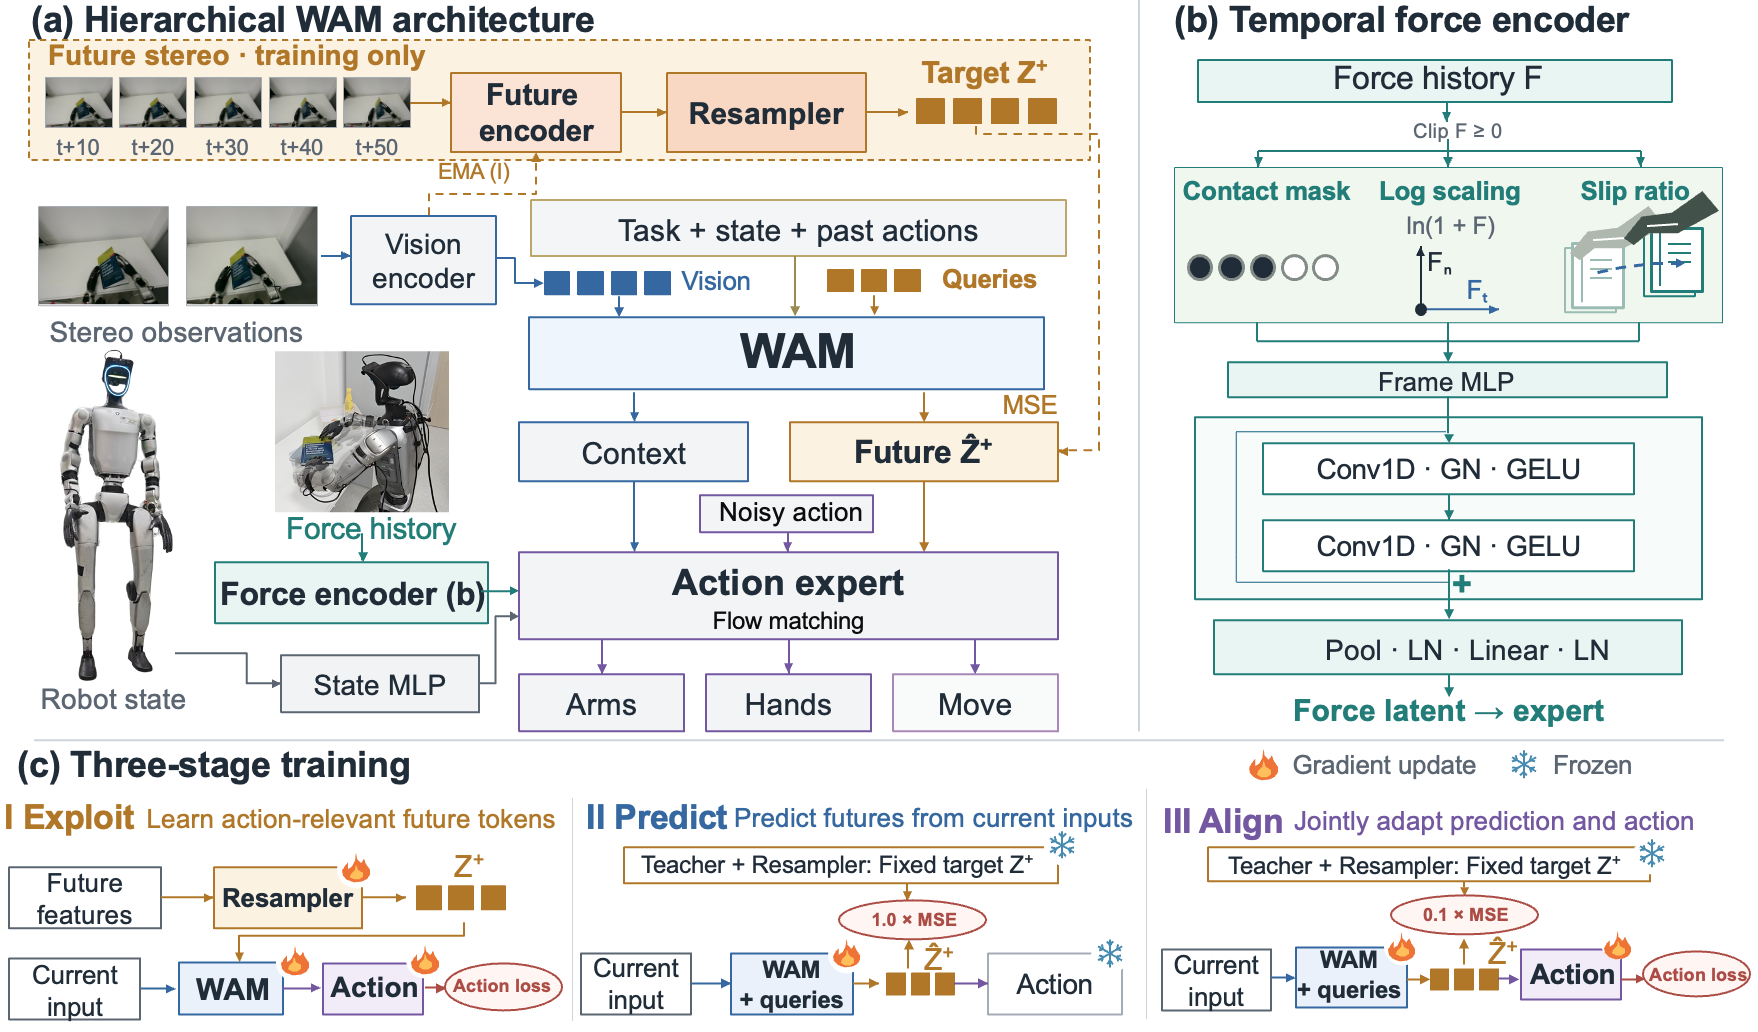
\includegraphics[width=\textwidth]{figures/frame2.png}
\caption{Overview of PHI. (a) A training-only future pathway constructs
$Z_t^{+}$ from future stereo observations, while the current interaction
context and future tokens condition the action policy. (b) A temporal force
encoder maps force history to a physical-interaction latent. (c) The
Exploit--Predict--Align training procedure.}
\label{fig:method_overview}
\end{figure}

% \subsection{Problem Formulation and PHI Overview}

% task definition
% overall policy
% three information streams:
%  current context / future representation / force representation

% We consider learning a policy for contact-rich bimanual manipulation from
% multimodal demonstrations. At each time step $t$, the robot observes a
% multi-view visual observation $o_t$, a language instruction $\ell$, the robot
% state $s_t$, a recent action history $\mathcal{H}^a_t$, and a history of force
% measurements $F_{t-K:t-1}$. The policy predicts an action
% chunk
% $A_t=[a_t,\ldots,a_{t+H-1}]$,
% where $H$ denotes the action horizon. We write the policy as

% \begin{equation}
%     A_t \sim
%     \pi_{\theta}
%     \left(
%         A_t \mid
%         o_t,\ell,s_t,\mathcal{H}^a_t,F_{t-K:t-1}
%     \right).
% \end{equation}

% The current observation, robot state, recent actions, and force history
% jointly provide the interaction context. The state token $s_t$ includes the
% current force measurements, while the recent force history is additionally
% processed by the temporal force encoder. We define the VLM context as
% $c_t=(o_t,\ell,s_t,\mathcal{H}^a_t)$.

% PHI augments the policy with a predictive future representation
% $\hat Z_t^{+}$ and a temporal force representation $z_t^{f}$. Together with
% the current vision-language representation $Z_t^{vl}$ and projected robot
% state $z_t^s$, they condition a flow-matching action expert:

% \begin{equation}
%     v_{\theta}
%     =
%     G_{\theta}
%     \left(
%         X_t^\tau,
%         \tau,
%         Z_t^{vl},
%         \hat Z_t^{+},
%         z_t^{f},
%         z_t^s
%     \right),
% \end{equation}

% where $X_t^\tau$ denotes an intermediate action trajectory along the flow
% path and $v_{\theta}$ is the predicted velocity field. Integrating this field
% produces the final action chunk.

% During training, future observations
% $\{o_{t+\Delta_m}\}_{m=1}^{M}$ construct the privileged target $Z_t^{+}$.
% At inference, this pathway is removed and the VLM predicts $\hat Z_t^{+}$
% from the current interaction context; Secs.~3.2--3.4 describe the complete
% training and deployment procedure.

% \subsection{Problem Formulation and PHI Overview}

% PHI adopts a two-stage architecture consisting of a World-Action Model (WAM) backbone and a flow-matching action expert. Given the current visual observation and language instruction, the WAM extracts a task-relevant visual-language representation and predicts a future representation from the current context. Meanwhile, the action expert directly receives the representations produced by the WAM together with the robot state and recent force history, and generates a chunk of future actions. The overall architecture and
% training schedule are illustrated in Fig.~\ref{fig:method_overview}. This architecture separates high-level visual reasoning and future prediction from low-level physical interaction modeling, while allowing both to jointly guide action generation.

% Formally, we define the current context as
% \begin{equation}
%     c_t = (o_t, \ell, s_t),
% \end{equation}
% where $o_t$ denotes the current visual observation, $\ell$ the language instruction, and $s_t$ the robot proprioceptive state. The WAM produces the current visual-language representation and the predicted future representation:
% \begin{equation}
%     Z_t^{vl} = E_{\mathrm{WAM}}(c_t),
%     \qquad
%     \hat{Z}_t^{+} = P_{\omega}(c_t),
% \end{equation}
% where $Z_t^{vl}$ captures the current task-relevant visual-language information, while $\hat{Z}_t^{+}$ represents the predicted future latent optimized for downstream action generation. In parallel, a temporal force encoder maps the recent force history
% \begin{equation}
%     \mathcal{F}_t =
%     \{F_{t-K+1}, \ldots, F_t\}
% \end{equation}
% to a force representation
% \begin{equation}
%     z_t^f = E_f(\mathcal{F}_t).
% \end{equation}
% The action expert then takes the WAM representations, robot state, and force representation as inputs and generates an action chunk
% \begin{equation}
%     A_t = \{a_t, \ldots, a_{t+H-1}\}
% \end{equation}
% through conditional flow matching:
% \begin{equation}
%     A_t \sim
%     \mathcal{G}_{\theta}
%     \left(
%         Z_t^{vl},
%         \hat{Z}_t^{+},
%         s_t,
%         z_t^f
%     \right).
% \end{equation}
% The future representation is constructed from privileged future observations during training, but is predicted solely from the current context at inference time, ensuring causal action generation.

% To learn this future representation progressively, PHI employs a three-stage training pipeline, \textit{Exploit, Predict, and Align}. The three stages progressively transfer action-grounded information from privileged future representations to the causal future prediction pathway, enabling the predicted future representation to effectively support action generation without requiring future observations at inference time. The detailed training procedure is presented in Sec.~3.3.

\subsection{Problem Formulation and PHI Overview}
PHI adopts a two-stage architecture consisting of a World Action Model (WAM)
and a flow-matching action expert. Given the current interaction context, the
WAM produces a task-relevant visual-language representation and predicts a
task oriented future representation. During training, a separate
\emph{Progressive Task Oriented Future Learning} module $\mathcal{T}_{\phi}$ constructs the
future representation target from privileged future observations, which is
then used to train the causal future prediction pathway. Meanwhile, the
action expert receives the representations produced by the WAM together
with the robot state and recent force history, and generates a chunk of
future actions. The overall architecture and training schedule are
illustrated in Fig.~\ref{fig:method_overview}.

Formally, we define the current interaction context as
$c_t=(o_t,\ell,s_t)$, where $o_t$ denotes the current visual observation,
$\ell$ the language instruction, and $s_t$ the robot proprioceptive state.
The WAM produces the current visual-language representation and the predicted
future representation:
\begin{equation}
    \left(
        Z_t^{vl},\hat{Z}_t^{+}
    \right)
    =
    \mathrm{WAM}_{\theta}(c_t).
\end{equation}
Here, $Z_t^{vl}$ denotes the current visual-language representation, while
$\hat{Z}_t^{+}$ denotes the predicted future representation. During training,
the Future Learning module
$\mathcal{T}_{\phi}$ uses privileged future observations to construct the
target future representation:
\begin{equation}
    Z_t^{+}
    =
    \mathcal{T}_{\phi}
    \left(
        o_{t+\Delta_1},\ldots,o_{t+\Delta_M}
    \right).
\end{equation}

In parallel, a temporal force encoder maps the recent force history
$\mathcal{F}_t=\{F_{t-K+1},\ldots,F_t\}$ to a force representation
$z_t^f=E_f(\mathcal{F}_t)$. The action expert then takes the WAM
representations, robot state, and force representation as inputs and
generates an action chunk $A_t=\{a_t,\ldots,a_{t+H-1}\}$ through conditional
flow matching, formulated as
$A_t \sim \mathcal{G}_{\theta}(Z_t^{vl},\hat{Z}_t^{+},s_t,z_t^f)$.
At inference time, the privileged future observations and
$\mathcal{T}_{\phi}$ are removed, and $\hat{Z}_t^{+}$ is predicted solely
from the current interaction context, enabling causal action generation.

Inspired by the effector-specific organization of the human motor cortex \cite{gordon2023somato}, we further structure the action expert with separate projectors for different body effectors. Specifically, the action space is decomposed into three groups, namely arms, hands, and move, each mapped to a dedicated action projector for generating its corresponding actions. This effector-specific decomposition reduces the learning burden of the high-dimensional action space and facilitates more effective optimization of coordinated humanoid actions.



% PHI adopts a two-stage architecture consisting of a World-Action Model (WAM) backbone and a flow-matching action expert. Given the current visual observation and language instruction, the WAM extracts a task-relevant visual-language representation and predicts a future representation from the current context. Meanwhile, the action expert directly receives the representations produced by the WAM together with the robot state and recent force history, and generates a chunk of future actions. The overall architecture and
% training schedule are illustrated in Fig.~\ref{fig:method_overview}.

% Formally, we define the current context as $c_t=(o_t,\ell,s_t)$, where $o_t$ denotes the current visual observation, $\ell$ the language instruction, and $s_t$ the robot proprioceptive state. The WAM produces the current visual-language representation and the predicted future representation:
% \begin{equation}
%     Z_t^{vl}=E_{\mathrm{WAM}}(c_t),
%     \qquad
%     \hat{Z}_t^{+}=P_{\omega}(c_t).
% \end{equation}
% Here, $Z_t^{vl}$ captures the current task-relevant visual-language information, while $\hat{Z}_t^{+}$ represents the predicted future latent optimized for downstream action generation. In parallel, a temporal force encoder maps the recent force history $\mathcal{F}_t=\{F_{t-K+1},\ldots,F_t\}$ to a force representation $z_t^f=E_f(\mathcal{F}_t)$.

% The action expert then takes the WAM representations, robot state, and force representation as inputs and generates an action chunk $A_t=\{a_t,\ldots,a_{t+H-1}\}$ through conditional flow matching:
% \begin{equation}
%     A_t \sim
%     \mathcal{G}_{\theta}
%     \left(
%         Z_t^{vl},
%         \hat{Z}_t^{+},
%         s_t,
%         z_t^f
%     \right).
% \end{equation}
% The future representation is constructed from privileged future observations during training, but is predicted solely from the current context at inference time, ensuring causal action generation.

% To learn this future representation progressively, PHI employs a three-stage training pipeline, \textit{Exploit, Predict, and Align}. The three stages progressively transfer action-grounded information from privileged future representations to the causal future prediction pathway, enabling the predicted future representation to effectively support action generation without requiring future observations at inference time. The detailed training procedure is presented in Sec.~3.3.



% A central goal of PHI is to provide the action policy with predictive
% information about how the ongoing interaction may evolve. The future
% representation should preserve information useful for downstream action
% generation rather than only visually predictable changes, while the policy
% must learn to exploit it as it is being learned. Jointly optimizing these
% objectives can entangle representation discovery, future prediction, and
% policy learning.

% PHI addresses this challenge with a progressive training strategy that
% transforms privileged future observations into a causal, action-grounded
% representation. The procedure consists of three stages:
% \emph{Exploit}, \emph{Predict}, and \emph{Align}. Stage I learns which future
% information is useful for action generation, Stage II learns to infer it from
% the current interaction context, and Stage III adapts the predicted
% representation together with the action policy. 

% \subsection{Progressive Action-Grounded Future Learning}

% We view PHI as a latent world model that predicts task-oriented future
% interaction states in representation space, with the latent space shaped
% directly by downstream action utility. The following sections describe the
% construction of the future target and the three training stages.

% % \subsubsection{Task Oriented Future Target}

% % 3.2.1 Privileged Future Target
% % 3.2.2 Future Predictor
% During training, PHI uses future observations as privileged information to
% construct a compact target representation. For each training sample at time
% $t$, we select $M$ future observation times $t+\Delta_1,\ldots,t+\Delta_M$.
% A teacher visual encoder $E_v^{\mathrm{EMA}}$ first extracts visual features
% from the corresponding future observations. The teacher encoder is updated by
% an exponential moving average of the online visual encoder and does not
% receive gradients directly. These features are then aggregated by a
% Perceiver-based resampler $R_\psi$ into a fixed number of latent tokens:

% \begin{equation}
%     Z_t^{+}
%     =
%     R_\psi
%     \left(
%         E_v^{\mathrm{EMA}}(o_{t+\Delta_1}),
%         \ldots,
%         E_v^{\mathrm{EMA}}(o_{t+\Delta_M})
%     \right),
% \end{equation}
% where $Z_t^{+}$ denotes the target future representation.

% The resampler compresses the future visual tokens into a fixed-size
% representation shaped by downstream action generation rather than
% future-image reconstruction. It serves as the privileged signal in Stage I
% and the supervision target for causal prediction; the resampler is optimized
% in Stage I and fixed later.



\subsection{Progressive Task Oriented Future Learning}

During training, PHI uses future observations as privileged information to construct a compact target representation through module
$\mathcal{T}_{\phi}$ which consists of an visual encoder
$E_v^{\mathrm{EMA}}$ and a Perceiver-based resampler $R_\psi$. For each
training sample at time $t$, we select $M$ future observation times
$t+\Delta_1,\ldots,t+\Delta_M$. The visual encoder
$E_v^{\mathrm{EMA}}$ first extracts visual features from the corresponding
future observations. Its initial parameters are copied from the online
visual encoder and subsequently updated using exponential moving average
(EMA), without receiving gradients directly. The extracted features are
then aggregated by the resampler $R_\psi$ into a fixed number of latent
tokens:
\begin{equation}
    Z_t^{+}
    =
    \mathcal{T}_{\phi}
    \left(
        o_{t+\Delta_1},\ldots,o_{t+\Delta_M}
    \right)
    =
    R_\psi
    \left(
        E_v^{\mathrm{EMA}}(o_{t+\Delta_1}),
        \ldots,
        E_v^{\mathrm{EMA}}(o_{t+\Delta_M})
    \right),
\end{equation}
where $Z_t^{+}$ denotes the target future representation. The resampler
compresses the future visual features into a compact, task oriented
representation, retaining information most useful for downstream action
generation. This provides the WAM with a compact and task oriented
prediction target, substantially reducing the difficulty of future
representation prediction.


% \subsection{Temporal Force Conditioning}

% The predictive future representation provides anticipatory information, but
% visual observations alone do not fully characterize contact dynamics. PHI
% therefore encodes recent physical interaction. Given
% $F_{t-K:t-1}\in\mathbb{R}^{K\times d_f}$, we apply a lightweight
% contact-aware transformation $\phi(\cdot)$ and temporal encoder $E_f$:

% \begin{equation}
%     \widetilde{F}_{t-K:t-1}
%     =
%     \phi(F_{t-K:t-1}),
%     \qquad
%     z_t^f
%     =
%     E_f
%     \left(
%         \widetilde{F}_{t-K:t-1}
%     \right).
% \end{equation}

% The temporal encoder maps recent contact evolution to a compact
% physical-interaction representation that conditions the action expert. Current
% force measurements enter through $s_t$, while the history encoder provides
% $z_t^f$; $\widehat{Z}_t^+$ supplies anticipatory visual context and $z_t^f$
% supplies reactive physical context. The privileged target $Z_t^{+}$ is
% constructed from future visual observations only. Implementation details are
% provided in the Appendix.

\subsection{Temporal Force Feedback}

Visual observations provide rich information about object geometry and
motion, but are insufficient to fully characterize physical interactions
during contact. PHI therefore encodes the recent force history
$\mathcal{F}_t=\{F_{t-K+1},\ldots,F_t\}$ to provide explicit information
about contact evolution. Each force measurement contains 20 channels. We
first apply non-negative clipping and logarithmic scaling to compress the
dynamic range, and additionally extract a binary contact mask and
tangential-to-normal force ratios to explicitly describe contact state and
potential sliding behavior. The resulting features are
\begin{equation}
    \widetilde{F}_t
    =
    \left[
        \log(1+\max(F_t,0));
        \mathbb{I}(F_t>1.0);
        F_t^{\mathrm{ratio}}
    \right]
    \in \mathbb{R}^{50},
\end{equation}
where $F_t^{\mathrm{ratio}}$ contains 10 tangential-to-normal force ratios,
computed as
\begin{equation}
    F_{t,i}^{\mathrm{ratio}}
    =
    \log\left(
        1+
        \frac{F_{t,i}^{\mathrm{tangential}}}
        {F_{t,i}^{\mathrm{normal}}+\epsilon}
    \right).
\end{equation}
Thus, each timestep is represented by $50$ force features,
combining continuous force magnitude with discrete contact information and
local force balance.

A temporal encoder $E_f$ aggregates the recent force feature sequence
$\widetilde{F}_{t-K+1},\ldots,\widetilde{F}_t$ into a force representation
$z_t^f=E_f(\widetilde{F}_{t-K+1},\ldots,\widetilde{F}_t)$, which is provided
directly to the action expert to complement the predictive visual
representation $\hat{Z}_t^{+}$ with temporally grounded physical information.

  % 3.4 Exploit–Predict–Align Training

  %     3.4.1 Exploit: Discover Action-Relevant Future Information

  %     3.4.2 Predict: Causal Future Prediction

  %     3.4.3 Align: Action-Driven Policy Adaptation
% \subsubsection{Stage I: Exploit Privileged Future Information}

% In the first stage, PHI learns to exploit privileged future information
% before attempting to predict it from the current observation. Given the
% target future representation $Z_t^{+}$ constructed in Sec.~3.2.1, we inject
% $Z_t^{+}$ into the VLM as privileged future tokens and reuse the notation
% $Z_t^{+}$ for the resulting future-conditioned representation passed to the
% action expert. This allows the action-generation pathway to condition on it
% together with the current vision-language representation, temporal force
% representation, and robot state:

% \begin{equation}
%     v_{\theta}
%     =
%     G_{\theta}
%     \left(
%         X_t^\tau,
%         \tau,
%         Z_t^{+},
%         z_t^{f},
%         z_t^{s}
%     \right),
% \end{equation}
% where $X_t^\tau$ denotes an intermediate action trajectory along the
% flow-matching path.

% We train the action expert using conditional flow matching. Given a
% demonstrated action chunk $A_t$ and a noise sample
% $\epsilon\sim\mathcal{N}(0,I)$, we sample a flow time $\tau$ from the
% training time distribution and construct an interpolated action trajectory:

% \begin{equation}
%     X_t^\tau
%     =
%     (1-\tau)A_t + \tau\epsilon,
% \end{equation}

% with target velocity

% \begin{equation}
%     u_t
%     =
%     \epsilon-A_t.
% \end{equation}

% The Stage-I objective is

% \begin{equation}
%     \mathcal{L}_{\mathrm{I}}
%     =
%     \mathcal{L}_{\mathrm{action}}
%     =
%     \mathbb{E}_{\tau,\epsilon,A_t}
%     \left[
%         \left\|
%         G_{\theta}
%         \left(
%             X_t^\tau,
%             \tau,
%             Z_t^{vl},
%             Z_t^{+},
%             z_t^{f},
%             z_t^{s}
%         \right)
%         - u_t
%         \right\|_2^2
%     \right].
% \end{equation}

% For the heterogeneous action space, we use lightweight body-part-specific
% output heads while sharing the multimodal conditioning across components;
% implementation details are deferred to the Appendix. The future resampler is
% optimized through the action objective, while the teacher is updated only by
% EMA. Thus, action gradients shape $Z_t^{+}$ into an action-grounded future
% latent space before causal prediction.

% \subsubsection{Stage II: Predict Action-Grounded Future Information}

% After Stage I, Stage II transfers the fixed target $Z_t^{+}$ from privileged
% future observations to the current interaction context. The online and
% teacher visual encoders, future resampler, and action-generation modules are
% fixed, while the VLM language/fusion layers and future query tokens remain
% trainable. Given $c_t$, the VLM produces

% \begin{equation}
%     \widehat{Z}_t^{+}
%     =
%     P_{\omega}(c_t),
% \end{equation}
% where $P_{\omega}$ denotes the future-prediction pathway of the VLM.

% The Stage-II objective is the latent-distillation loss:

% \begin{equation}
%     \mathcal{L}_{\mathrm{II}}
%     =
%     \mathcal{L}_{\mathrm{future}}
%     =
%     \left\|
%         \widehat{Z}_t^{+}
%         -
%         \operatorname{sg}
%         \left(
%             Z_t^{+}
%         \right)
%     \right\|_2^2,
% \end{equation}
% where $\operatorname{sg}(\cdot)$ denotes stop-gradient. The VLM never
% accesses the future observations used to construct $Z_t^{+}$; they only
% provide supervision. Since the target is shaped by action utility, Stage II
% distills control-relevant future information into a causal predictor rather
% than predicting arbitrary future visual content.

% \subsubsection{Stage III: Policy-Level Alignment}

% Although Stage II teaches the VLM to reproduce the action-grounded target,
% latent matching alone does not guarantee optimal interaction with the final
% policy. Stage III therefore couples future prediction with downstream action
% generation.

% In Stage III, the action expert receives the predicted future representation
% rather than the privileged target representation:

% \begin{equation}
%     v_{\theta}
%     =
%     G_{\theta}
%     \left(
%         X_t^\tau,
%         \tau,
%         Z_t^{vl},
%         \widehat{Z}_t^{+},
%         z_t^{f},
%         z_t^{s}
%     \right),
% \end{equation}

% with $\widehat{Z}_t^{+}=P_{\omega}(c_t)$.

% In Stage III, latent matching is relaxed rather than removed: the predictor
% and action policy are jointly adapted under action supervision while a weak
% alignment regularizer preserves the connection to the privileged target. The
% Stage-III objective is

% \begin{equation}
%     \mathcal{L}_{\mathrm{III}}
%     =
%     \mathcal{L}_{\mathrm{action}}
%     +
%     \lambda_{\mathrm{align}}\mathcal{L}_{\mathrm{future}},
% \end{equation}

% where $\lambda_{\mathrm{align}}$ is small relative to the Stage-II
% supervision. The visual encoders and target resampler remain fixed, while the
% VLM language/fusion layers, future queries, and action policy are adapted.
% Together, Exploit--Predict--Align learns what future information matters for
% control, how to predict it from the current context, and how to adapt it to
% action generation.

% \subsection{Three-Stage Training: Exploit, Predict, and Align}

% PHI is trained with a three-stage curriculum, namely \textit{Exploit,
% Predict, and Align}, which progressively transfers action-relevant
% information from privileged future observations to a causal future
% prediction pathway. We first learn an action-grounded future target using
% privileged observations, then train the model to predict this target from
% the current context, and finally remove the explicit target supervision so
% that future prediction is directly optimized by downstream action
% generation.

% \textbf{Stage I: Exploit.}
% We first train the action-generation pathway with the privileged future
% representation $Z_t^{+}$ introduced in Sec.~3.2. Since $Z_t^{+}$ is
% constructed from future observations during training, it provides direct
% access to future information and allows the model to learn which future
% features are useful for action generation. Given an action chunk $A_t$ and
% a flow time $\tau$, we sample $\epsilon\sim\mathcal{N}(0,I)$ and construct
% the intermediate action state
% \begin{equation}
%     X_t^\tau = (1-\tau)A_t + \tau\epsilon,
%     \qquad
%     u_t = \epsilon - A_t.
% \end{equation}
% The flow-matching action expert predicts the target velocity conditioned on
% the current visual-language representation, privileged future
% representation, robot state, and force representation:
% \begin{equation}
%     \mathcal{L}_{\mathrm{I}}
%     =
%     \mathbb{E}_{\tau,\epsilon,A_t}
%     \left[
%         \left\|
%         \mathcal{G}_{\theta}
%         \left(
%             X_t^\tau,
%             \tau,
%             Z_t^{vl},
%             Z_t^{+},
%             s_t,
%             z_t^f
%         \right)
%         - u_t
%         \right\|_2^2
%     \right].
% \end{equation}
% The future resampler is optimized through this action objective, while the
% teacher visual encoder is updated only by EMA. Consequently, the
% privileged future representation is shaped directly by downstream action
% utility.

% \textbf{Stage II: Predict.}
% After learning the action-grounded target, we train the causal future
% prediction pathway to recover the same representation from the current
% context. Specifically, the future predictor produces
% \begin{equation}
%     \hat{Z}_t^{+} = P_{\omega}(c_t),
% \end{equation}
% where $c_t=(o_t,\ell,s_t)$. The privileged target $Z_t^{+}$ is kept fixed
% and provides supervision through latent distillation:
% \begin{equation}
%     \mathcal{L}_{\mathrm{II}}
%     =
%     \left\|
%         \hat{Z}_t^{+}
%         -
%         \operatorname{sg}\!\left(Z_t^{+}\right)
%     \right\|_2^2.
% \end{equation}
% Here, $\operatorname{sg}(\cdot)$ denotes stop-gradient. The predictor only
% receives the current context and never accesses future observations,
% thereby learning to infer the action-relevant future information
% causally.

% \textbf{Stage III: Align.}
% Finally, we replace the privileged representation with the predicted
% future representation and optimize future prediction through downstream
% action generation. The action expert now takes
% $\hat{Z}_t^{+}=P_{\omega}(c_t)$ as its future condition:
% \begin{equation}
%     \mathcal{L}_{\mathrm{III}}
%     =
%     \mathbb{E}_{\tau,\epsilon,A_t}
%     \left[
%         \left\|
%         \mathcal{G}_{\theta}
%         \left(
%             X_t^\tau,
%             \tau,
%             Z_t^{vl},
%             \hat{Z}_t^{+},
%             s_t,
%             z_t^f
%         \right)
%         - u_t
%         \right\|_2^2
%     \right].
% \end{equation}
% No explicit future-target loss is applied in this stage. Instead, the
% action loss directly propagates through $\hat{Z}_t^{+}$ into the future
% prediction pathway, allowing the predicted future representation to
% adapt to the information most useful for action generation. The target
% representation and its teacher encoder remain fixed, while the causal
% future prediction and action-generation pathways are optimized jointly.

% Overall, the three stages progressively learn what future information is
% useful for action generation, how to predict it from the current context,
% and how to align the prediction with the downstream control objective.


\subsection{Three-Stage Training: Exploit, Predict, and Align}

PHI is trained with a three-stage curriculum, namely \textit{Exploit,
Predict, and Align}, which progressively transfers task oriented
information from privileged future observations to a causal future
prediction pathway. We first learn an task oriented future target using
privileged observations, then train the model to predict this target from
the current context, and finally replace the privileged target with the predicted representation, jointly optimizing future prediction and downstream action generation.

% \textbf{Stage I: Exploit.}
% We first train the task oriented pathway with the privileged future
% representation $Z_t^{+}$. Since $Z_t^{+}$ is
% constructed from future observations during training, it provides direct
% access to future information and allows the model to learn which future
% features are useful for action generation. Given a demonstrated action
% chunk $A_t$ and a noise sample $\epsilon\sim\mathcal{N}(0,I)$, we sample a
% flow time $\tau$ and construct
% \begin{equation}
%     X_t^\tau=(1-\tau)A_t+\tau\epsilon,
%     \qquad
%     u_t=\epsilon-A_t.
% \end{equation}
% The action expert is then optimized with the conditional flow-matching
% objective
% \begin{equation}
%     \mathcal{L}_{\mathrm{I}}
%     =
%     \mathbb{E}_{\tau,\epsilon,A_t}
%     \left[
%         \left\|
%         \mathcal{G}_{\theta}
%         \left(
%             X_t^\tau,\tau,
%             Z_t^{vl},Z_t^{+},s_t,z_t^f
%         \right)
%         -u_t
%         \right\|_2^2
%     \right].
% \end{equation}
% The future resampler is optimized through this action objective, while the
% teacher visual encoder is updated only by EMA. Thus, the privileged future
% representation is shaped directly by downstream action utility.
\textbf{Stage I: Exploit.}
We first learn the task oriented future target from privileged future
observations. Since $Z_t^{+}$ is constructed from future observations during
training, it provides privileged access to future information and allows the
model to identify features useful for downstream action generation. Given a
demonstrated action chunk $A_t$ and a noise sample
$\epsilon\sim\mathcal{N}(0,I)$, we sample a flow time $\tau$ and construct
$X_t^\tau=(1-\tau)A_t+\tau\epsilon$ with target velocity
$u_t=\epsilon-A_t$. The action expert is optimized with the conditional
flow-matching objective
\begin{equation}
    \mathcal{L}_{\mathrm{I}}
    =
    \mathbb{E}_{\tau,\epsilon,A_t}
    \left[
        \left\|
        \mathcal{G}_{\theta}
        \left(
            X_t^\tau,\tau,
            Z_t^{vl},Z_t^{+},s_t,z_t^f
        \right)
        -u_t
        \right\|_2^2
    \right].
\end{equation}
During this stage, the resampler $R_\psi$ is optimized through the action
objective, while the teacher visual encoder $E_v^{\mathrm{EMA}}$ is updated
only by exponential moving average. Consequently, the target future
representation $Z_t^{+}=\mathcal{T}_{\phi}(\cdot)$ is shaped to retain
task oriented information that is useful for downstream action generation.


% \textbf{Stage II: Predict.}
% After learning the action-grounded target, we train the causal future
% prediction pathway to recover the same representation from the current
% context. Specifically, the future predictor produces
% \begin{equation}
%     \hat{Z}_t^{+}=P_{\omega}(c_t),
%     \qquad
%     c_t=(o_t,\ell,s_t),
% \end{equation}
% and is supervised by the fixed privileged target through latent
% distillation:
% \begin{equation}
%     \mathcal{L}_{\mathrm{II}}
%     =
%     \left\|
%         \hat{Z}_t^{+}
%         -
%         \operatorname{sg}\!\left(Z_t^{+}\right)
%     \right\|_2^2.
% \end{equation}
% Here, $\operatorname{sg}(\cdot)$ denotes stop-gradient. The predictor only
% receives the current context and never accesses future observations, while
% $Z_t^{+}$ provides training-time supervision. Since the target has already
% been shaped by action utility in Stage I, Stage II distills
% control-relevant future information rather than arbitrary future visual
% content.

\textbf{Stage II: Predict.}
After learning the task oriented future target, we train the WAM to predict
the same representation from the current interaction context. Specifically,
given $c_t=(o_t,\ell,s_t)$, the WAM produces
$\left(Z_t^{vl},\hat{Z}_t^{+}\right)=\mathrm{WAM}_{\theta}(c_t)$,
where $\hat{Z}_t^{+}$ is supervised by the fixed privileged target through
latent distillation:
\begin{equation}
    \mathcal{L}_{\mathrm{II}}
    =
    \left\|
        \hat{Z}_t^{+}
        -
        \operatorname{sg}\!\left(Z_t^{+}\right)
    \right\|_2^2.
\end{equation}
Here, $\operatorname{sg}(\cdot)$ denotes stop-gradient. The WAM receives
only the current interaction context and never accesses future observations,
while $Z_t^{+}$ provides training-time supervision. Since $Z_t^{+}$ has been
shaped by downstream action generation in Stage I, Stage II learns to predict
task oriented future information from the current context.


\textbf{Stage III: Align.}
Finally, we replace the privileged future representation $Z_t^{+}$ with the
predicted future representation $\hat{Z}_t^{+}$ and jointly optimize future
prediction and action generation, while keeping the target module
$\mathcal{T}_{\phi}$ fixed. The overall objective combines the losses from the
previous two stages:
\begin{equation}
\mathcal{L}{\mathrm{III}}
=
\mathcal{L}{\mathrm{I}}
+
\tau\mathcal{L}{\mathrm{II}},
\qquad
\tau=0.1.
\end{equation}
Here, $\mathcal{L}{\mathrm{I}}$ uses $\hat{Z}_t^{+}$ as the future
representation for action generation, while $\mathcal{L}{\mathrm{II}}$
maintains prediction consistency with the privileged target $Z_t^{+}$.


\subsection{Multimodal Action Generation and Causal Inference}

% At deployment, the WAM takes only the current context $c_t$ and produces
% the current visual-language representation $Z_t^{vl}$ and the predicted
% future representation $\widehat{Z}_t^+=P_{\omega}(c_t)$. The recent force
% history $\mathcal{F}_t$ is encoded into $z_t^f=E_f(\mathcal{F}_t)$, while the
% robot state $s_t$ is directly provided to the action expert. The privileged
% future-observation pathway is removed entirely, ensuring causal inference
% at deployment. These representations condition the flow-matching action
% expert defined in Eq.~(2), with lightweight body-part-specific heads used
% for the heterogeneous action space. Implementation details are provided
% in the Appendix.

% Action generation starts from Gaussian noise at the terminal point of the
% flow, i.e., $\epsilon\sim\mathcal{N}(0,I)$ and
% $X_t^{1}=\epsilon$. The learned velocity field is integrated backward over $N$ inference steps,
% with $1=\tau_0>\tau_1>\cdots>\tau_N=0$. Denoting the predicted velocity at
% step $n$ by $\hat{u}_t^{\,n}
% =
% \mathcal{G}_{\theta}(X_t^{\tau_n},\tau_n,Z_t^{vl},\widehat{Z}_t^+,s_t,z_t^f)$,
% the trajectory is updated as
% \begin{equation}
%     X_t^{\tau_{n+1}}
%     =
%     X_t^{\tau_n}
%     +
%     (\tau_{n+1}-\tau_n)\hat{u}_t^{\,n}.
% \end{equation}
% The final action chunk is given by $A_t=X_t^{\tau_N}$.The robot executes
% the first action or a short prefix of the chunk, after which the policy is
% recomputed from updated observations, yielding receding-horizon
% closed-loop execution.


At deployment, the WAM takes the current context $c_t$ and produces the
current visual-language representation $Z_t^{vl}$ and the predicted future
representation $\hat{Z}_t^+$. The recent force history $\mathcal{F}_t$ is
encoded into $z_t^f$, and the robot state $s_t$ is directly provided to the
action expert. The privileged future-observation pathway and target module
$\mathcal{T}_{\phi}$ are removed, ensuring causal inference. The flow-matching
action expert then generates an action chunk $A_t$, which is executed using
Real-Time Chunking (RTC)~\cite{black2025realtimeexecutionactionchunking}.
RTC asynchronously predicts the next action chunk while executing the current
one, using action inpainting to smoothly connect consecutive chunks. 


% \subsection{Multimodal Action Generation and Causal Inference}




%   % 3.5 Multimodal Action Generation

%   %     ├── flow matching

%   %     ├── multi-head action

%   %     └── inference
% At deployment, the WAM produces $Z_t^{vl}$ and
% $\widehat{Z}_t^+=P_{\omega}(c_t)$, while the temporal force and state encoders
% produce $z_t^f=E_f(\phi(F_{t-K:t-1}))$ and $z_t^s=E_s(s_t)$. These
% representations condition the flow-matching action expert in Eq.~(2);
% lightweight body-part-specific heads handle the heterogeneous action space.
% Implementation details are provided in the Appendix.

% At deployment, the privileged future-observation pathway is removed. The VLM
% uses only $c_t$ to predict $\widehat{Z}_t^+$, and the force encoder uses the
% observed history $F_{t-K:t-1}$ to produce $z_t^f$.

% Action generation begins from a Gaussian action trajectory at the noise end of
% the flow:

% \begin{equation}
%     \epsilon \sim \mathcal{N}(0,I),
%     \qquad
%     X_t^{\tau_0}=\epsilon,
%     \qquad
%     \tau_0=1.
% \end{equation}

% The learned velocity field is then integrated backward over $N$ inference
% steps, with $1=\tau_0>\tau_1>\cdots>\tau_N=0$:

% \begin{equation}
%     \hat u_t^{\,n}
%     =
%     G_{\theta}
%     \left(
%         X_t^{\tau_n},
%         \tau_n,
%         Z_t^{vl},
%         \widehat{Z}_t^+,
%         z_t^f,
%         z_t^s
%     \right),
% \end{equation}

% \begin{equation}
%     X_t^{\tau_{n+1}}
%     =
%     X_t^{\tau_n}
%     +
%     (\tau_{n+1}-\tau_n)\hat u_t^{\,n},
%     \qquad
%     n=0,\ldots,N-1.
% \end{equation}

% The final action chunk is given by

% \begin{equation}
%     A_t=X_t^{\tau_N}.
% \end{equation}

% The robot executes the first action or a short prefix, then recomputes the
% policy from updated observations for receding-horizon closed-loop execution.


%加入伪代码，王天虹V1版


% \section{EXPERIMENTS}
% \label{sec:experiments}

% We conduct experiments to answer the following three questions:
% \textbf{(1)} Can PHI improve policy performance as the complexity of physical interaction increases?
% \textbf{(2)} Can PHI generalize to unseen objects and visual conditions?
% \textbf{(3)} What makes the learned future representation useful for contact-rich manipulation?

% \subsection{Experimental Setup}
% \label{sec:experimental_setup}

% \paragraph{Robot Platform.}
% We evaluate all methods on a Unitree G1 humanoid with 29 degrees of freedom, equipped with two 6-DoF BrainCo dexterous hands with tactile sensing and a binocular RGB camera mounted on the head. The policy predicts an action chunk of $H=50$ steps and executes it in a receding-horizon manner. The predicted actions are tracked by ULC, a unified loco-manipulation controller that converts root velocity, body height, torso, and dual-arm commands into whole-body joint targets~\cite{sun2025ulc}.

% \paragraph{Task Suite.}
% We evaluate five real-robot tasks spanning different levels of physical interaction: \textit{Walk to Table}, \textit{Place Bottle}, \textit{Open Book}, \textit{Place Cube}, and \textit{Place Book Straight}. As shown in Fig.~\ref{fig:tasks}, the suite progresses from no-contact locomotion and object grasping to sustained bimanual contact and friction-regulated manipulation.
% Table~\ref{tab:task_characteristics} summarizes the key characteristics of each task, including the required contact mode and bimanual coordination. We use three contact levels to describe the increasing interaction requirements: $\mathrm{L1}$ for no intentional object contact, $\mathrm{L2}$ for grasping or sustained contact, and $\mathrm{L3}$ for friction-regulated contact.
% Representative tactile traces are shown in Fig.~\ref{fig:tactile_traces} (Appendix~\ref{app:tactile_traces}). These traces characterize the interaction patterns in our suite.

% \begin{figure}[t]
%     \centering
%     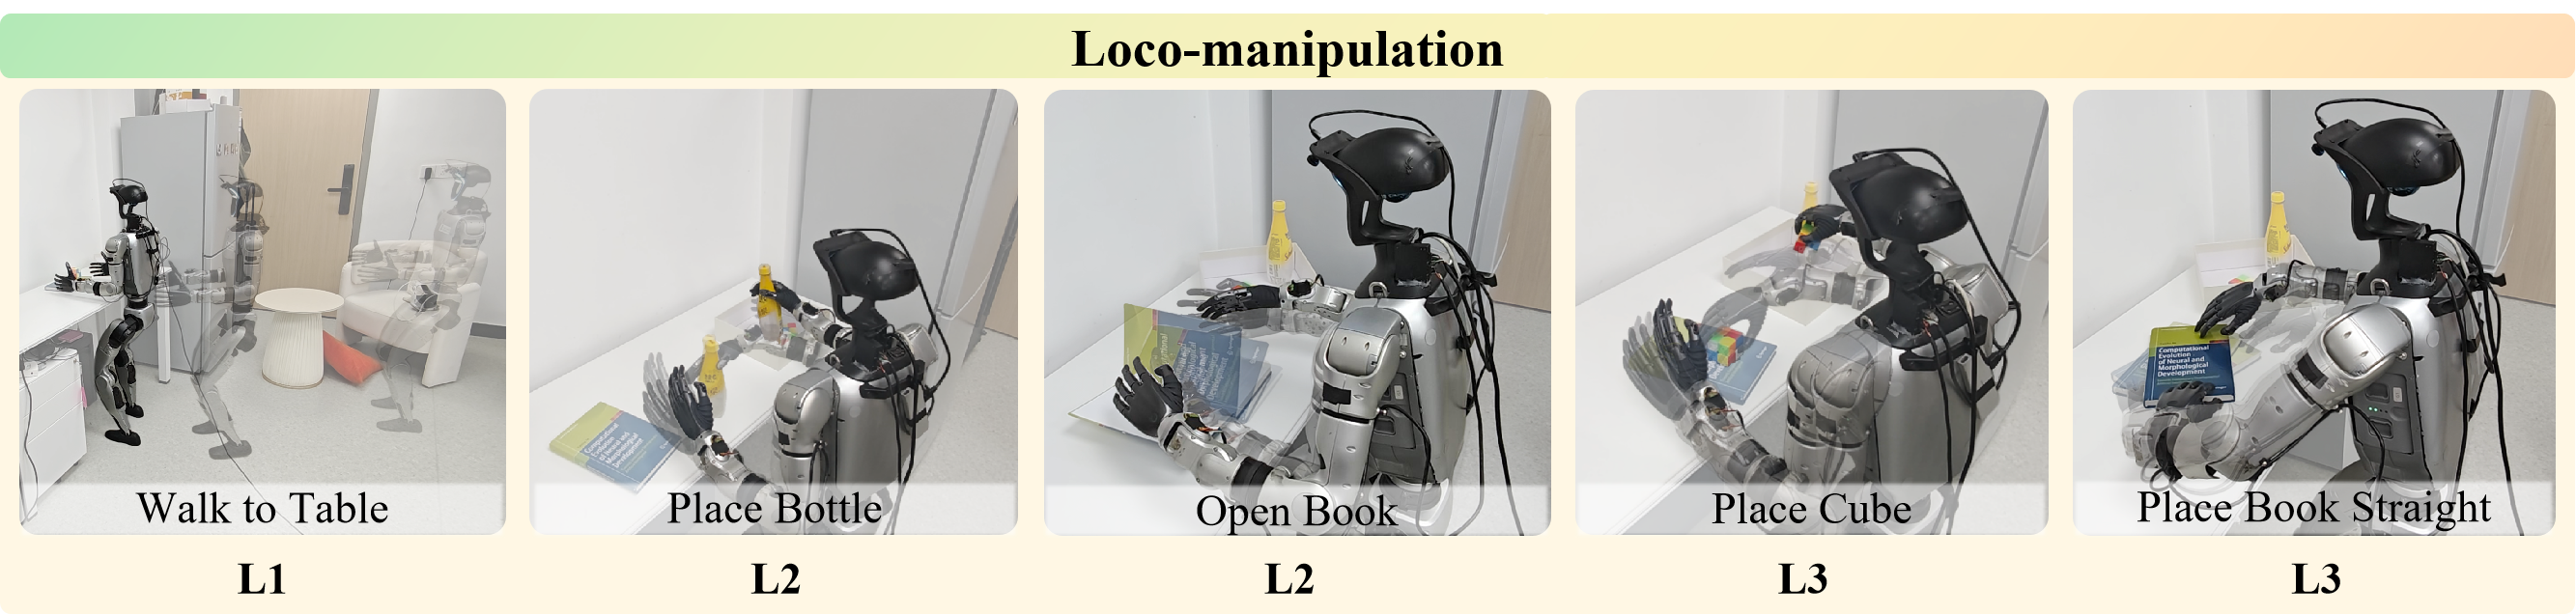
\includegraphics[width=\textwidth]{figures/tasks.png}
%     \caption{
%     Real-robot task suite used for evaluation.
%     The five tasks span different levels of physical interaction, from no-contact locomotion and object grasping to sustained bimanual contact and friction-regulated manipulation.
%     }
%     \label{fig:tasks}
% \end{figure}

% % \begin{table}[t]
% %     \centering
% %     \small
% %     \renewcommand{\arraystretch}{1.05}
% %     \setlength{\tabcolsep}{5pt}
% %     \caption{
% %     Task characteristics and contact complexity.
% %     $\mathrm{L1}$--$\mathrm{L3}$ indicate increasing levels of physical interaction required for successful task completion.
% %     }
% %     \label{tab:task_characteristics}
% %     \begin{tabular}{lcccc}
% %         \toprule
% %         \textbf{Task}
% %         & \textbf{Level}
% %         & \textbf{Dual-arm}
% %         & \textbf{Contact}
% %         & \textbf{Necessary contact mode} \\
% %         \midrule
% %         Walk to Table
% %         & L1 & -- & -- & No contact \\
% %         Place Bottle
% %         & L2 & -- & $\bullet$ & Grasp \\
% %         Open Book
% %         & L2 & $\bullet\bullet$ & $\bullet\bullet$ & Sustained contact \\
% %         Place Cube
% %         & L3 & -- & $\bullet\bullet\bullet$ & Friction regulation \\
% %         Place Book Straight
% %         & L3 & $\bullet\bullet\bullet$ & $\bullet\bullet\bullet$ & Friction regulation \\
% %         \bottomrule
% %     \end{tabular}
% % \end{table}


% \begin{table}[t]
%     \centering
%     \small
%     \renewcommand{\arraystretch}{1.05}
%     \setlength{\tabcolsep}{5pt}
%     \caption{
%    Task characteristics and contact complexity.
%     $\mathrm{L1}$--$\mathrm{L3}$ indicate increasing levels of physical interaction required for successful task completion.
%     }
%     \label{tab:task_characteristics}
%     \begin{tabular}{llcl}
%         \toprule
%         \textbf{Task}
%         & \textbf{Group}
%         & \textbf{Arms}
%         & \textbf{Necessary contact mode} \\
%         \midrule
%         Walk to Table
%         & L1 & -- & No intentional hand--object contact \\
%         Place Bottle
%         & L2 & Unimanual & Grasp \\
%         Open Book
%         & L2 & Bimanual & Sustained support \\
%         Place Cube
%         & L3 & Unimanual & Friction-regulated grasp \\
%         Place Book Straight
%         & L3 & Bimanual & Sliding and rotation \\
%         \bottomrule
%     \end{tabular}
% \end{table}

% \paragraph{Baselines.}
% We compare PHI with three representative methods: $\pi_0$~\cite{black2024pi0}, $\pi_{0.5}$~\cite{black2025pi05}, and VLA-JEPA~\cite{sun2026vlajepa}. These baselines cover strong vision-language-action policies and predictive representation-based approaches relevant to our setting. All methods use the same training data, robot platform, task definitions, action space, controller, and evaluation protocol.

% \paragraph{Evaluation Protocol.}
% For in-domain evaluation, each task is evaluated over 30 real-robot trials with randomized initial conditions. For object-centric tasks, object position and orientation are varied across trials, and the same sequence of initial conditions is used for all methods. For \textit{Place Book Straight}, we partition the table into six regions---left, upper left, upper center, center, upper right, and right---and conduct five trials per region, with the book placed at a random position and orientation within the assigned region. For \textit{Place Bottle}, the 30 trials are evenly divided among an uncluttered setting, a book placed beside the target, and a book placed beneath it. A trial is successful only when the complete task objective is achieved and the final state remains stable for a predefined holding period. For book manipulation, the final position and orientation must additionally satisfy task-specific tolerances.

% \subsection{Main Results}
% \label{sec:main_results}

% Table~\ref{tab:main_results} reports the success rates of PHI and the baseline methods across five real-robot tasks. Tasks are listed in the same order as in Fig.~\ref{fig:tasks}. The overall success rate is computed across 150 trials per method, with 30 trials per task. PHI achieves an overall success rate of $82.0\%$,
% representing a $39.8\%$ relative improvement over $\pi_0$, the strongest baseline overall at $58.7\%$.

% \begin{wrapfigure}{r}{0.60\textwidth}
%     \centering
%     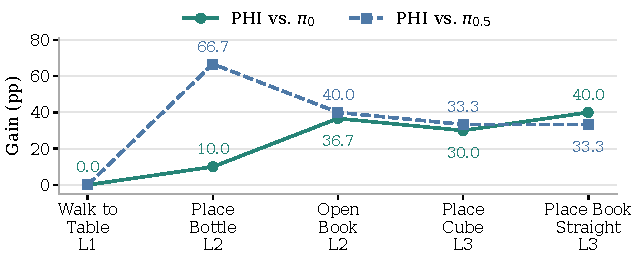
\includegraphics[width=\linewidth]{figures/gain_over_pi0.pdf}
%     \captionsetup{font=small,skip=2pt}
%     \caption{PHI's gains over $\pi_0$ and $\pi_{0.5}$ (pp).}
%     \label{fig:contact_gain}
% \end{wrapfigure}
% The two bimanual book tasks provide a focused comparison
% of performance on sustained-support and sliding-and-rotation
% manipulation.
% On \textit{Open Book}, PHI achieves $86.7\%$ success,
% compared with $50.0\%$ for $\pi_0$ and $46.7\%$ for
% $\pi_{0.5}$.
% On \textit{Place Book Straight}, PHI achieves $76.7\%$
% success, compared with $43.3\%$ for $\pi_{0.5}$ and
% $36.7\%$ for $\pi_0$.
% PHI also outperforms the baselines on the two unimanual
% object-placement tasks, \textit{Place Bottle} and
% \textit{Place Cube}.
% On \textit{Place Bottle}, PHI achieves $76.7\%$ success,
% compared with $66.7\%$ for $\pi_0$ and $10.0\%$ for
% $\pi_{0.5}$.
% On \textit{Place Cube}, PHI achieves $70.0\%$ success,
% compared with $40.0\%$ for $\pi_0$ and $36.7\%$ for
% $\pi_{0.5}$.
% On \textit{Walk to Table}, which requires no intentional
% hand--object contact, PHI, $\pi_0$, and $\pi_{0.5}$ all
% achieve $100\%$ success; no additional gain over these
% two baselines is observed under this evaluation.
% Figure~\ref{fig:contact_gain} summarizes the per-task
% gains over $\pi_0$ and $\pi_{0.5}$.

% % \noindent
% % \begin{minipage}{\linewidth}
% %     \begin{minipage}[t]{0.38\linewidth}
% %         \vspace{0pt}
% %         % \textbf{Contact-level comparison.}
% %         Figure~\ref{fig:contact_gain} shows PHI's gains
% %         over $\pi_0$ and $\pi_{0.5}$.
% %     \end{minipage}
% %     \hfill
% %     \begin{minipage}[t]{0.61\linewidth}
% %         \vspace{0pt}
% %         \centering
% %         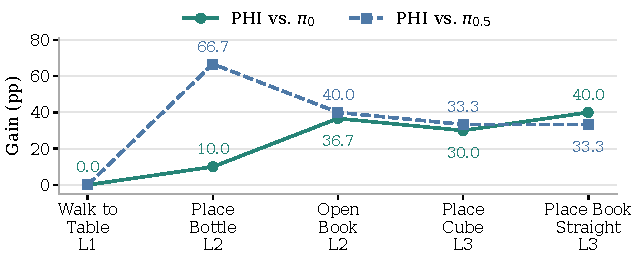
\includegraphics[width=\linewidth]{figures/gain_over_pi0.pdf}
% %         \captionsetup{font=small,skip=2pt}
% %         \captionof{figure}{PHI's gains over $\pi_0$ and $\pi_{0.5}$ (pp).}
% %         \label{fig:contact_gain}
% %     \end{minipage}
% % \end{minipage}

% % The two bimanual book tasks provide a focused comparison of performance on sustained-support and sliding-and-rotation manipulation. On \textit{Open Book}, PHI achieves $86.7\%$ success, compared with $50.0\%$ for $\pi_0$ and $46.7\%$ for $\pi_{0.5}$. 
% % On \textit{Place Book Straight}, PHI achieves $76.7\%$ success, compared with $43.3\%$ for $\pi_{0.5}$ and $36.7\%$ for $\pi_0$. 
% % PHI also outperforms the baselines on the two unimanual object-placement tasks, \textit{Place Bottle} and \textit{Place Cube}. On \textit{Place Bottle}, PHI achieves $76.7\%$ success, compared with $66.7\%$ for $\pi_0$ and $10.0\%$ for $\pi_{0.5}$. On \textit{Place Cube}, PHI achieves $70.0\%$ success, compared with $40.0\%$ for $\pi_0$ and $36.7\%$ for $\pi_{0.5}$. On \textit{Walk to Table}, which requires no intentional hand--object contact, PHI, $\pi_0$, and $\pi_{0.5}$ all achieve $100\%$ success; no additional gain over these two baselines is observed under this evaluation. Figure~\ref{fig:contact_gain} summarizes the per-task gains over $\pi_0$ and $\pi_{0.5}$.

% Under our adaptation and evaluation protocol, VLA-JEPA achieves $6.7\%$ success on \textit{Walk to Table} and $0.0\%$ on each manipulation task, yielding an overall success rate of $1.3\%$. One possible explanation is the mismatch in embodiment and control between its original setup and our platform. The original work uses end-effector motion commands and binary gripper commands, with real-world experiments conducted on a single Franka arm equipped with a parallel-jaw gripper~\cite{sun2026vlajepa}. Adapting this formulation to a humanoid platform with two dexterous hands and whole-body control may introduce additional learning challenges, although we have not isolated the effect of this mismatch on performance.
% % First, PHI, $\pi_0$, and $\pi_{0.5}$ all achieve $100\%$ success on the no-contact \textit{Walk to Table} task, 
% % whereas VLA-JEPA achieves $6.7\%$. On the four object-manipulation tasks, 
% % PHI achieves $70.0$--$86.7\%$ success and is the best-performing method in every case.
% % Across all five tasks, PHI obtains an average success rate of $82.0\%$, 
% % a \textbf{$39.7\%$ relative improvement} over the strongest baseline average of $58.7\%$ from $\pi_0$.

% % Second, contact introduces failure modes that cannot be reliably resolved from visual observations alone. In \textit{Place Bottle}, the robot must grasp and transport the bottle without applying excessive or unstable contact forces that may knock the bottle over. This makes stable grasping and force regulation critical even though the task itself does not require complex bimanual manipulation. PHI achieves $76.7\%$ success, substantially outperforming $\pi_{0.5}$ ($10.0\%$) and $\pi_0$ ($66.7\%$). The larger gap over $\pi_{0.5}$ suggests that contact-sensitive manipulation can be particularly challenging for policies relying primarily on visual observations.

% % \textit{Place Cube} requires a unimanual grasp-and-place of a small cube. The policy must precisely control the grasp location to avoid inducing unwanted rotation, while modulating fingertip pinch force to regulate friction so that the cube does not slip. PHI achieves $70.0\%$ success, compared with $40.0\%$ for $\pi_0$ and $36.7\%$ for $\pi_{0.5}$.

% % The difficulty increases substantially in \textit{Open Book}, where successful execution requires accurate placement of both hands, coordinated bimanual motion, and appropriate regulation of the interaction forces. The robot must simultaneously lift the cover with one hand and stabilize the book with the other, making small errors in either hand position or applied force sufficient to cause failure. PHI achieves $86.7\%$ success, compared with $50.0\%$ for $\pi_0$ and $46.7\%$ for $\pi_{0.5}$.

% % Finally, \textit{Place Book Straight} requires the policy to adapt to the book's initial pose: in some configurations a single sliding motion is sufficient, while others require translating the book and then rotating it to the target pose. PHI achieves $76.7\%$ success, substantially higher than $\pi_{0.5}$ ($43.3\%$) and $\pi_0$ ($36.7\%$).

% Figure~\ref{fig:qualitative_execution} (Appendix) shows selected successful PHI executions across the five tasks.

% \begin{table*}[t]
% \centering
% \small
% \renewcommand{\arraystretch}{1.05}
% \setlength{\tabcolsep}{2pt}
% \caption{
% Success rates (\%) across the real-robot task suite, in the same order as Fig.~\ref{fig:tasks}.
% Values in parentheses denote successful trials over the number of trials.
% The best result in each column is shown in bold.
% The green value reports the relative improvement over the strongest baseline average, computed from the unrounded aggregate success rates.
% }
% \label{tab:main_results}
% \begin{tabular}{lcccccc}
% \toprule
% \textbf{Method} & \shortstack{\textbf{Walk to}\\\textbf{Table}} & \shortstack{\textbf{Place}\\\textbf{Bottle}} & \shortstack{\textbf{Open}\\\textbf{Book}} & \shortstack{\textbf{Place}\\\textbf{Cube}} & \shortstack{\textbf{Place Book}\\\textbf{Straight}} & \textbf{Avg.} \\
% \midrule
% $\pi_{0.5}$~{\scriptsize(\citealp{black2025pi05})} & \textbf{100.0} {\scriptsize(30/30)} & 10.0 {\scriptsize(3/30)} & 46.7 {\scriptsize(14/30)} & 36.7 {\scriptsize(11/30)} & 43.3 {\scriptsize(13/30)} & 47.3 \\
% $\pi_0$~{\scriptsize(\citealp{black2024pi0})} & \textbf{100.0} {\scriptsize(30/30)} & 66.7 {\scriptsize(20/30)} & 50.0 {\scriptsize(15/30)} & 40.0 {\scriptsize(12/30)} & 36.7 {\scriptsize(11/30)} & 58.7 \\
% VLA-JEPA~{\scriptsize(\citealp{sun2026vlajepa})} & 6.7 {\scriptsize(2/30)} & 0.0 {\scriptsize(0/30)} & 0.0 {\scriptsize(0/30)} & 0.0 {\scriptsize(0/30)} & 0.0 {\scriptsize(0/30)} & 1.3 \\
% \midrule
% \rowcolor{gray!15}
% \textbf{PHI (Ours)} & \textbf{100.0} {\scriptsize(30/30)} & \textbf{76.7} {\scriptsize(23/30)} & \textbf{86.7} {\scriptsize(26/30)} & \textbf{70.0} {\scriptsize(21/30)} & \textbf{76.7} {\scriptsize(23/30)} & \textbf{82.0} {\color{green!50!black}\textbf{(+39.8\%)}} \\
% \bottomrule
% \end{tabular}
% \end{table*}



% \subsection{Generalization to Unseen Objects and Visual Conditions}
% \label{sec:generalization}

% % We next evaluate whether PHI can generalize beyond the visual and physical conditions observed during training. We consider two types of distribution shifts: visual distractors that change the scene composition, and unseen objects that change both object appearance and physical interaction properties. These experiments test whether the policy can adapt to the underlying manipulation state rather than relying on memorized visual patterns.
% We next evaluate PHI under visual and physical conditions
% that differ from those observed during training.
% We consider two types of distribution shifts:
% visual distractors that change the scene composition,
% and unseen objects that differ in appearance and
% physical interaction properties.
% These experiments assess task performance under changes
% in scene composition and object identity.

% \paragraph{Robustness to Visual Distractors.}
% % We first evaluate the robustness of PHI to changes in scene composition. During evaluation, several irrelevant objects with different appearances are placed around the target object, while the manipulation objective and target object remain unchanged. The identities and positions of the distractors are varied across trials, preventing the policy from relying on a fixed scene layout.
% % As shown in Fig.~\ref{fig:generalization}(a), PHI maintains a high success rate under visual clutter, achieving $70.0\%$ (7/10) compared with $30.0\%$ (3/10) for $\pi_0$ and $10.0\%$ (1/10) for $\pi_{0.5}$. Relative to the in-domain rate of $76.7\%$ (23/30), this is a drop of 6.7 percentage points on a smaller 10-trial evaluation. The scenes below panel (a) show one in-domain layout and three clutter examples.
% We evaluate PHI under changes in scene composition by
% placing several irrelevant objects with different
% appearances around the target object, while keeping
% the target object and manipulation objective unchanged.
% Distractor identities and positions vary across trials
% to test transfer across varied scene layouts.
% As shown in Fig.~\ref{fig:generalization}(a), PHI achieves
% $70.0\%$ success (7/10) under visual clutter, compared
% with $30.0\%$ (3/10) for $\pi_0$ and $10.0\%$ (1/10)
% for $\pi_{0.5}$.
% For reference, PHI achieves $76.7\%$ (23/30) in-domain.
% The corresponding $95\%$ Wilson confidence intervals
% are $39.7\%$--$89.2\%$ under clutter and
% $59.1\%$--$88.2\%$ in-domain.
% PHI has the highest observed success rate among the
% evaluated methods under clutter, although the small
% sample size limits the precision of this comparison.
% The scenes below panel (a) show one in-domain layout
% and three clutter examples.

% \paragraph{Generalization to Unseen Objects.}
% We further evaluate object-level generalization using three books that never appear in the training data: \textit{Linear Algebra Done Right}, \textit{Federated Learning}, and \textit{Deep Learning}. The held-out books differ from the training objects in cover appearance, thickness, and material properties, with one book being a softcover rather than a hardcover. These variations introduce both visual and physical distribution shifts, since changes in thickness and compliance can alter the forces required for grasping, bracing, sliding, and opening.

% We evaluate both \textit{Place Book Straight} and \textit{Open Book} using the same three held-out books, with 10 trials per book. Figure~\ref{fig:generalization}(b,c) reports the 30-trial aggregate for each task. The scenes below each panel show the seen book followed by the three held-out books. On \textit{Place Book Straight}, PHI achieves $60.0\%$ success (18/30), compared with $30.0\%$ for $\pi_{0.5}$ and $23.3\%$ for $\pi_0$, a $100\%$ relative improvement over the strongest baseline. On \textit{Open Book}, PHI reaches $56.7\%$ (17/30), while both $\pi_0$ and $\pi_{0.5}$ achieve $33.3\%$, a $70.0\%$ relative improvement.

% PHI retains an aggregate advantage on both tasks, but performance is lower than on the training-domain books. These results support transfer to the evaluated books rather than robustness to every appearance or contact-property change.

% \begin{figure}[t]
%     \centering
%     \includegraphics[width=\linewidth]
%     {figures/generalization_combined.png}
%     \caption{
%     Generalization to visual distractors and unseen books.
%     (a) \textit{Place Book Straight} under clutter.
%     (b,c) Straightening and opening held-out books.
%     }
%     \label{fig:generalization}
% \end{figure}


% \Needspace{20\baselineskip}
% \subsection{Ablation Studies}
% \label{sec:ablations}

% \begin{wraptable}{r}{0.55\textwidth}
%     \centering
%     \small
%     \setlength{\tabcolsep}{3pt}
%     \renewcommand{\arraystretch}{1.08}
%     \captionsetup{font=small,skip=4pt}
%     \caption{Ablation success rates (\%) on two contact-rich
%     tasks.}
%     \label{tab:ablations}
%     \begin{tabular}{@{}lcc@{}}
%         \toprule
%         \textbf{Variant}
%         & \shortstack{\textbf{Place Book}\\\textbf{Straight}}
%         & \shortstack{\textbf{Open}\\\textbf{Book}} \\
%         \midrule
%         \textbf{PHI} & \textbf{76.7} & \textbf{86.7} \\
%         w/o force conditioning & 68.4 & 75.3 \\
%         w/o predictive future latent & 50 & 65.8 \\
%         \bottomrule
%     \end{tabular}
% \end{wraptable}
% We conduct ablation studies to examine the contributions
% of temporal force conditioning and predictive future
% latents. We evaluate both components on
% \textit{Open Book} and \textit{Place Book Straight},
% which require continuous contact, bimanual coordination,
% and fine-grained interaction control. Each ablation
% removes one component while keeping the remaining
% architecture and training procedure unchanged.

% % \noindent
% % \begin{minipage}{\linewidth}
% %     \begin{minipage}[t]{0.42\linewidth}
% %         \vspace{0pt}
% %         We conduct ablation studies to examine the contributions
% %         of temporal force conditioning and predictive future
% %         latents. We evaluate both components on
% %         \textit{Open Book} and \textit{Place Book Straight},
% %         which require continuous contact, bimanual coordination,
% %         and fine-grained interaction control. Each ablation
% %         removes one component while keeping the remaining
% %         architecture and training procedure unchanged.
% %     \end{minipage}
% %     \hfill
% %     \begin{minipage}[t]{0.55\linewidth}
% %         \vspace{0pt}
% %         \centering
% %         \small
% %         \setlength{\tabcolsep}{3pt}
% %         \renewcommand{\arraystretch}{1.08}
% %         \captionof{table}{Ablation success rates (\%) on two contact-rich tasks. Each variant removes one component while keeping the remaining architecture unchanged. Dashes indicate unreported results.}
% %         \label{tab:ablations}
% %         \begin{tabular}{@{}lcc@{}}
% %             \toprule
% %             \textbf{Variant}
% %             & \shortstack{\textbf{Place Book}\\\textbf{Straight}}
% %             & \shortstack{\textbf{Open}\\\textbf{Book}} \\
% %             \midrule
% %             \textbf{PHI} & \textbf{76.7} & \textbf{86.7} \\
% %             w/o force conditioning & -- & -- \\
% %             w/o predictive future latent & -- & -- \\
% %             \bottomrule
% %         \end{tabular}
% %     \end{minipage}
% % \end{minipage}
% % \par\medskip

% % \paragraph{Effect of Force Conditioning.}

% % We first remove temporal force conditioning while keeping the visual observations and predictive future latent unchanged. As shown in Table~\ref{tab:ablations}, removing force conditioning degrades the performance on both contact-rich tasks. Without force information, the policy must infer the physical interaction state primarily from visual observations, making it difficult to determine whether contact has been successfully established, whether the applied force is sufficient for sliding, and when the interaction should stop. The degradation is particularly evident in \textit{Place Book Straight}, where successful execution requires continuous regulation of normal and tangential forces during sliding. These results demonstrate that temporal force information provides complementary state information that cannot be reliably recovered from vision alone.

% \paragraph{Effect of Temporal Force Encoding.}

% We remove the temporal force encoder and its dedicated history representation $z_t^f$, while retaining current force measurements in $s_t$ and keeping the visual observations and predictive future latent unchanged. Current force information therefore remains available through both the VLM state context and the projected robot state $z_t^s$. This ablation isolates the contribution of explicit force-history modeling beyond instantaneous force inputs. As shown in Table~\ref{tab:ablations}, removing temporal force encoding degrades performance on both contact-rich tasks. Without temporal force encoding, the policy lacks the dedicated representation of recent force evolution that can help distinguish contact establishment, sustained sliding, and interaction termination. The degradation is particularly evident in \textit{Place Book Straight}, where successful execution requires continuous regulation of normal and tangential forces during sliding. These results suggest that modeling force history provides useful information about contact dynamics beyond the current visual observations and instantaneous force measurements.


% \paragraph{Effect of Predictive Future Latents.}

% We next remove the predictive future latent while retaining force conditioning. This ablation evaluates whether explicitly anticipating future visual states provides benefits beyond current observations and force feedback. Removing the predictive component leads to degraded performance on both tasks, with more frequent delayed transitions, overshooting, and failures to appropriately switch between manipulation phases.

% The effect is particularly important for \textit{Place Book Straight}, where different initial poses can require different future action sequences. Depending on the initial configuration, the robot may only need to slide the book, or may need to translate it first and subsequently rotate it. 
% % A policy based only on the current observation and force state must infer the appropriate future action online, whereas the predictive latent provides an explicit representation of the expected future visual state.
% PHI explicitly conditions the policy on a predictive representation learned with future-observation supervision during training. At deployment, this representation is inferred solely from the currently available interaction context and may help distinguish subsequent manipulation phases; it does not provide access to actual future observations.

% \begin{figure}[!tbh]
%     \centering
%     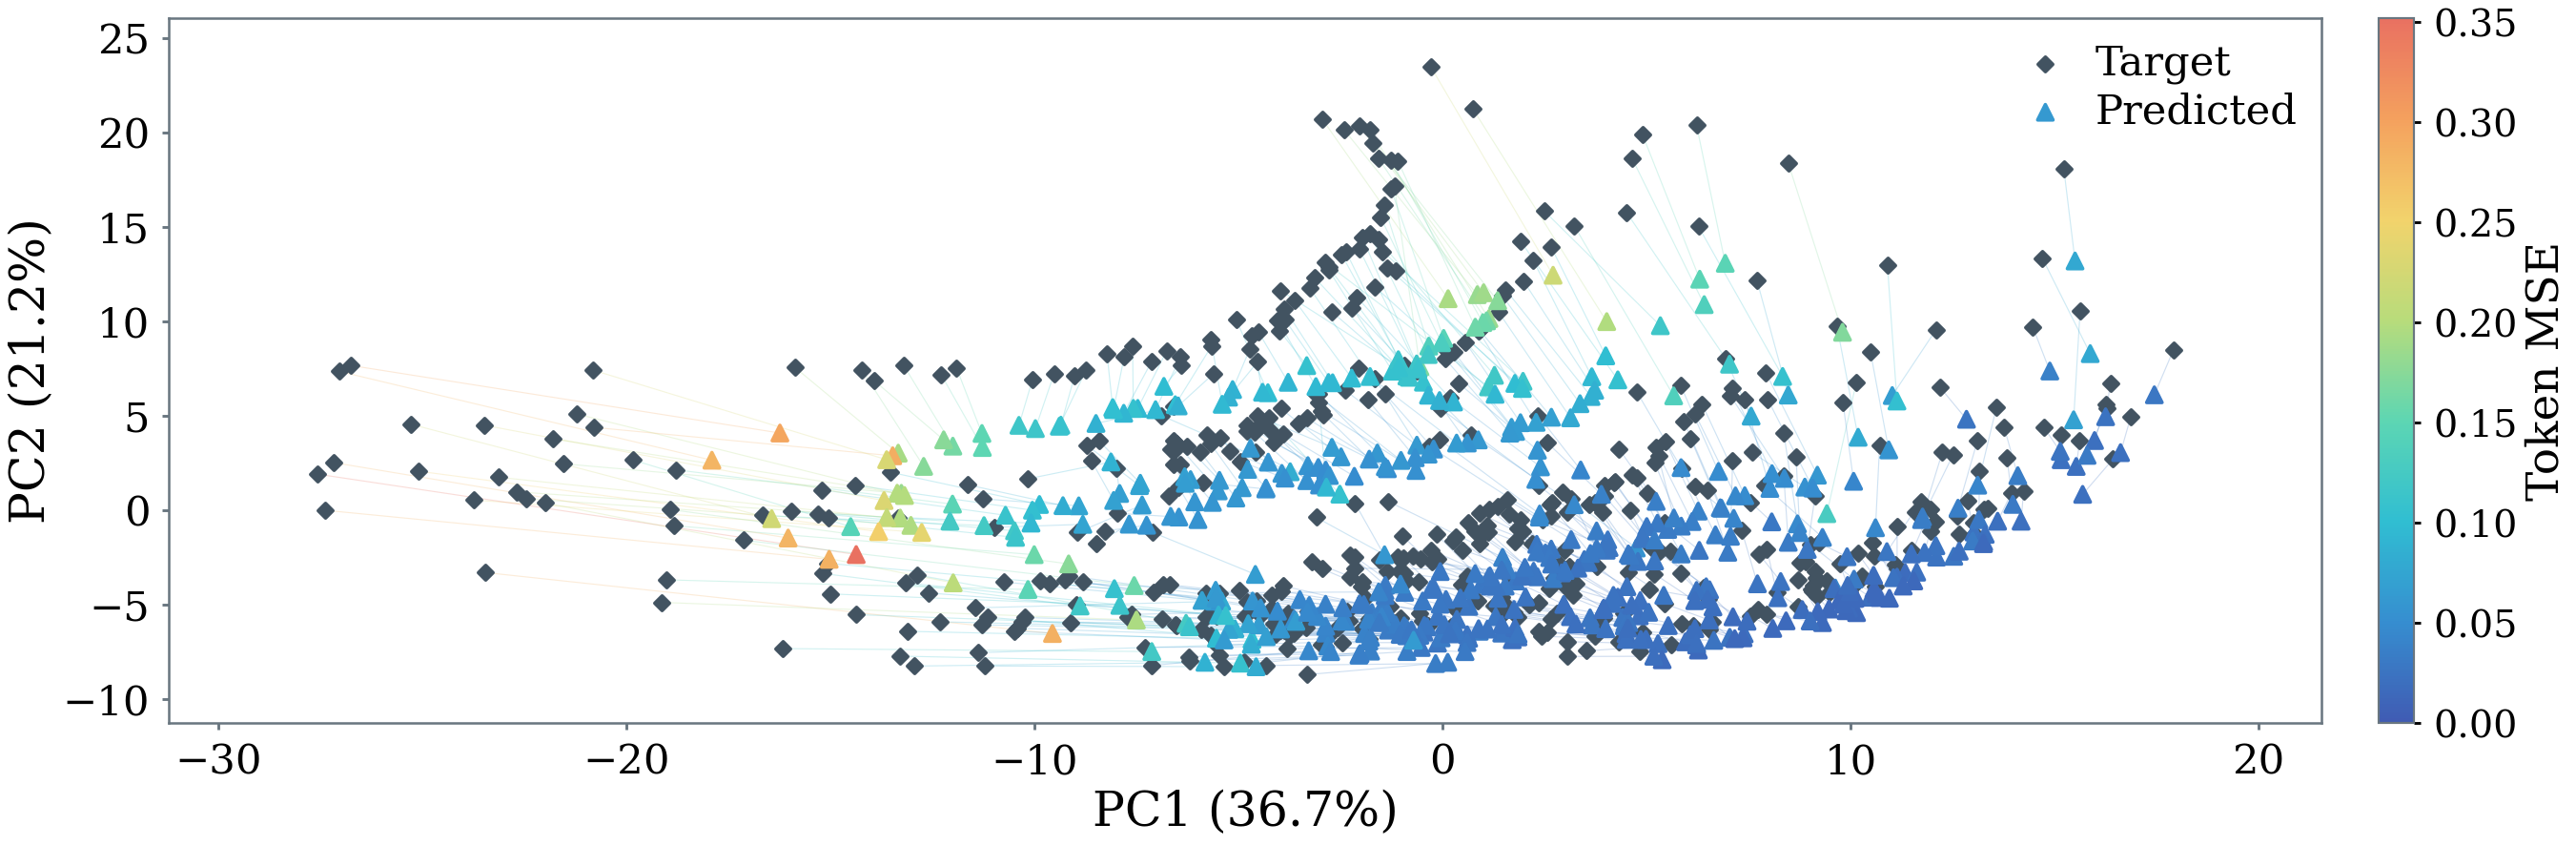
\includegraphics[width=\linewidth]{figures/PCA.png}
%     \caption{Joint PCA of predicted and target future-latent tokens for a single exported frame. Lines connect matched queries; colors indicate per-query MSE in the original feature space.}
%     \label{fig:latent_analysis}
% \end{figure}

% \begin{figure}[!tbh]
%     \centering
%     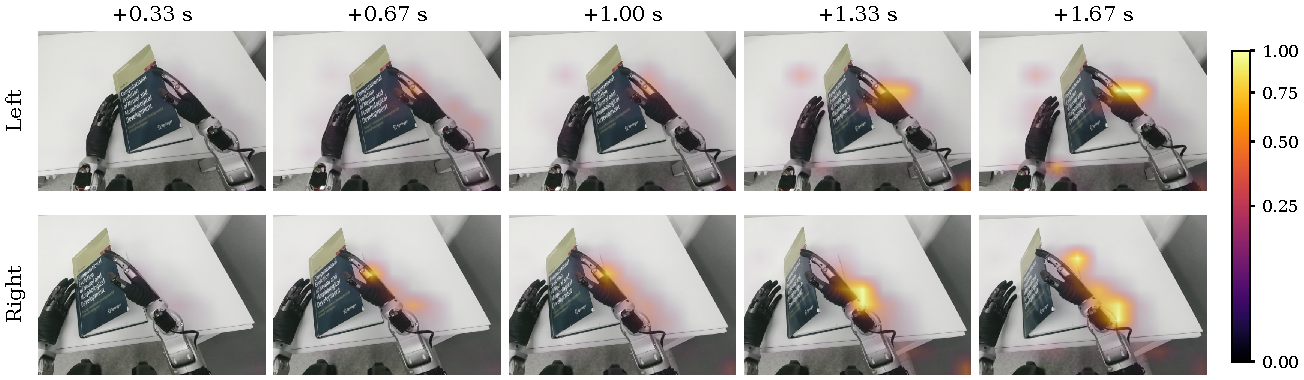
\includegraphics[width=.90\linewidth]{figures/perceiver_attention_focus.pdf}
%     \caption{Final-layer attention of the training-only teacher Perceiver over privileged future stereo observations during target construction. Rows correspond to the left and right cameras, and columns show future time offsets. }
%     \label{fig:attention_analysis}
% \end{figure}

% Figure~\ref{fig:latent_analysis} presents a single-sample visualization of predicted and target future-latent tokens for one exported frame, with the target representation extracted from five future stereo observations. The predicted and target tokens are jointly projected onto a shared PCA basis fitted to their concatenation. The first two principal components explain $36.7\%$ and $21.2\%$ of the variance in this sample's pooled tokens, respectively. Diamonds and triangles denote target and predicted tokens, and lines connect matching query pairs. Predicted tokens are colored by per-query mean squared error, averaged over the 2048 feature dimensions in the original representation space. The reported cosine similarity of $0.9690$ is computed in the original feature space for each matched predicted--target token pair and then averaged over the 512 queries in this sample. It indicates within-sample representation agreement, rather than average prediction quality across the test set, and does not by itself establish that the model captures contact transitions or improves action quality. Figure~\ref{fig:latent_alignment} further reports per-query original-space errors for this same sample.

% % To further understand this behavior, Fig.~\ref{fig:latent_analysis} presents a joint PCA visualization of the predicted and target future-latent tokens, with the target representation extracted from five future stereo observations. Both sets are projected into a shared two-dimensional space, where the first two principal components explain $36.7\%$ and $21.2\%$ of the total variance, respectively. Diamonds and triangles denote target and predicted tokens, lines connect matching query pairs, and predicted tokens are colored by their mean squared error in the original feature space. The predicted and target representations exhibit similar overall distribution patterns, consistent with a mean cosine similarity of $0.9690$. Original-space errors are further reported in Fig.~\ref{fig:latent_alignment}.

% % We additionally visualize the attention maps of the action prediction network in Fig.~\ref{fig:attention_analysis}. The policy primarily attends to the manipulated object and the interacting hands, indicating that the learned representation focuses on regions directly related to future action generation. Together, the ablation and qualitative analyses suggest that predictive future representations provide action-relevant information about the upcoming manipulation state, complementing the instantaneous physical-state information provided by force conditioning.
% Figure~\ref{fig:attention_analysis} visualizes the final-layer attention of the teacher Perceiver as it aggregates privileged future stereo observations to construct the training-time target representation. In the displayed example, attention is concentrated on the manipulated object and interacting hands, illustrating which visual regions the teacher emphasizes during target construction. These maps describe the training-only teacher pathway and do not establish a causal contribution of the attended regions to action outputs. PHI is designed to combine the resulting predictive visual representation with the recent force dynamics captured by the temporal force encoder; the effect on policy performance must be assessed through controlled ablations.

\section{EXPERIMENTS}
\label{sec:experiments}

We conduct experiments to answer the following three questions:
\textbf{(1)} Can PHI improve policy performance as the complexity of physical interaction increases?
\textbf{(2)} Can PHI generalize to unseen objects and visual conditions?
\textbf{(3)} What makes the learned future representation useful for humanoid bimanual dexterous manipulation?

\subsection{Experimental Setup}
\label{sec:experimental_setup}

\paragraph{Robot Platform.}
We evaluate all methods on a Unitree G1 humanoid with 29 degrees of freedom, equipped with two 6-DoF BrainCo dexterous hands with tactile sensing and a head-mounted binocular RGB camera. The policy predicts an action chunk of $H=50$ steps in a receding-horizon manner. Actions are tracked by ULC, a unified loco-manipulation controller that converts root velocity, body height, torso, and dual-arm commands into whole-body joint targets~\cite{sun2025ulc}.



\paragraph{Task Suite and Dataset.}
We evaluate five real-robot tasks spanning different levels of physical interaction: \textit{Walk to Table}, \textit{Place Bottle}, \textit{Open Book}, \textit{Place Cube}, and \textit{Place Book Straight}. As shown in Fig.~\ref{fig:tasks}, the suite progresses from no-contact locomotion and object grasping to sustained bimanual contact and friction-regulated manipulation.
Table~\ref{tab:task_characteristics} summarizes the key characteristics of each task, including the required contact mode and bimanual coordination. We use three contact levels to describe the increasing interaction requirements: $\mathrm{L1}$ for no intentional object contact, $\mathrm{L2}$ for grasping or sustained contact, and $\mathrm{L3}$ for friction-regulated contact.
Representative tactile traces are shown in Fig.~\ref{fig:tactile_traces} (Appendix~\ref{app:tactile_traces}). These traces characterize the interaction patterns in our suite. 
For each task, we collect 100 demonstration trajectories through
VR teleoperation. The collected data follow the LeRobot format
~\cite{cadene2024lerobot}, including synchronized observations, robot states,
actions, and tactile measurements. From tactile measurements, we extract 20-dimensional normal and tangential force features from both hands, which are included in the 49-dimensional robot state and used to construct a 10-step force history for the temporal force encoder.

\begin{figure}[ht]
    \centering
    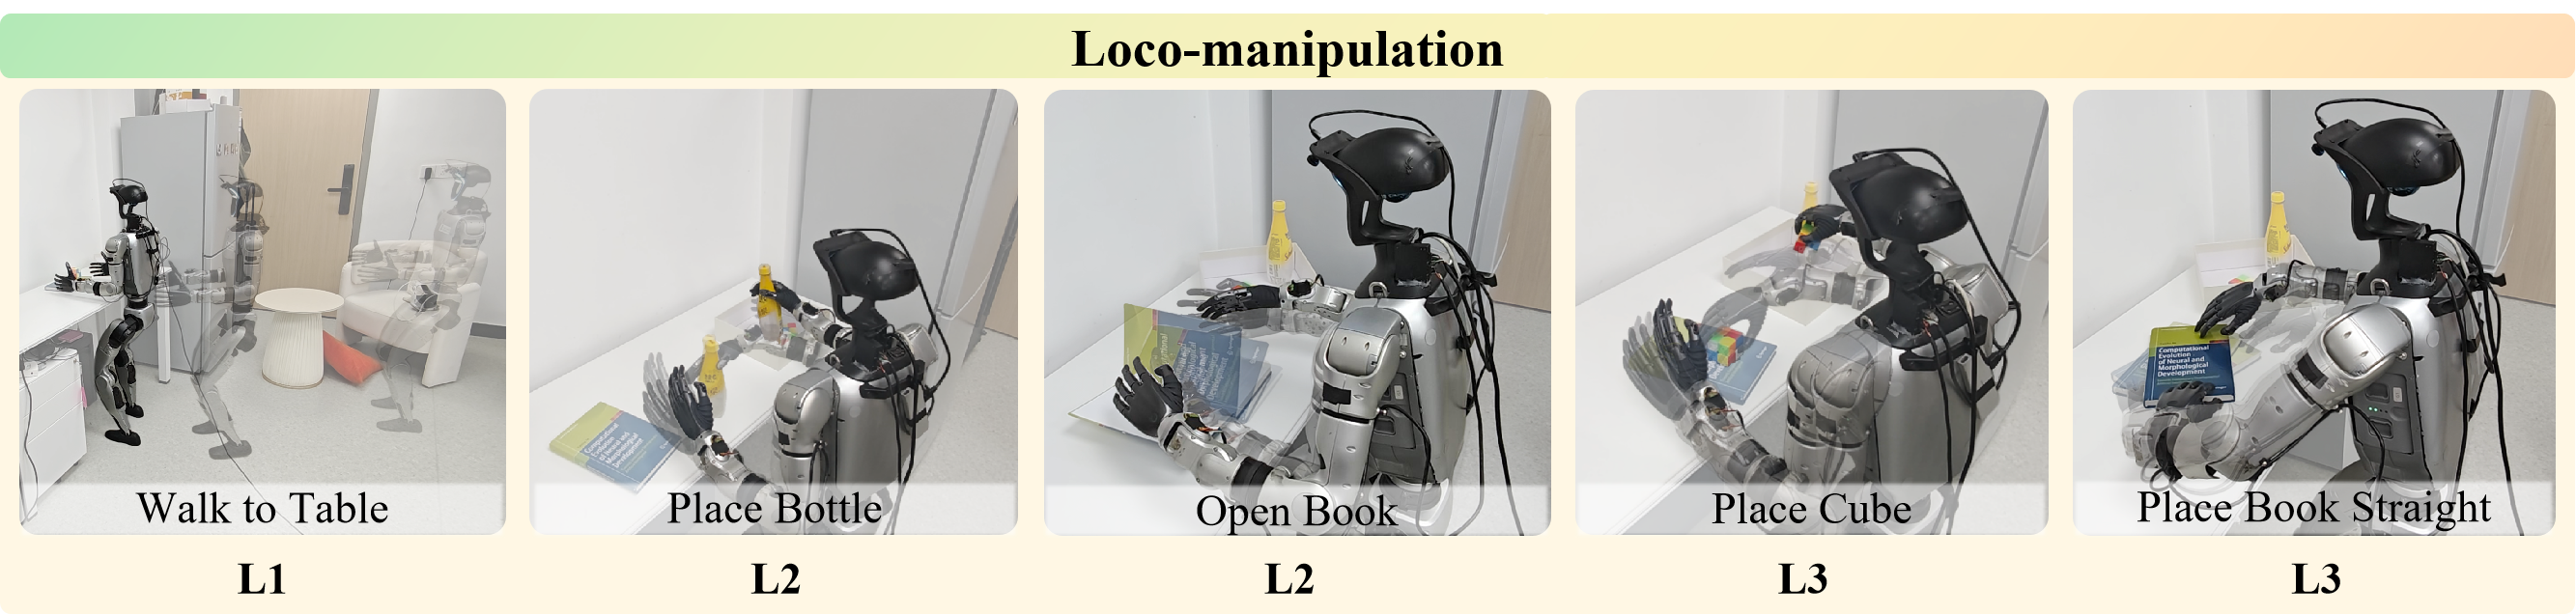
\includegraphics[width=\textwidth]{figures/tasks.png}
    \caption{
    Real-robot task suite used for evaluation.
    The five tasks span different levels of physical interaction, from no-contact locomotion and object grasping to sustained bimanual contact and friction-regulated manipulation.
    }
    \label{fig:tasks}
\end{figure}

% \begin{table}[t]
%     \centering
%     \small
%     \renewcommand{\arraystretch}{1.05}
%     \setlength{\tabcolsep}{5pt}
%     \caption{
%     Task characteristics and contact complexity.
%     $\mathrm{L1}$--$\mathrm{L3}$ indicate increasing levels of physical interaction required for successful task completion.
%     }
%     \label{tab:task_characteristics}
%     \begin{tabular}{lcccc}
%         \toprule
%         \textbf{Task}
%         & \textbf{Level}
%         & \textbf{Dual-arm}
%         & \textbf{Contact}
%         & \textbf{Necessary contact mode} \\
%         \midrule
%         Walk to Table
%         & L1 & -- & -- & No contact \\
%         Place Bottle
%         & L2 & -- & $\bullet$ & Grasp \\
%         Open Book
%         & L2 & $\bullet\bullet$ & $\bullet\bullet$ & Sustained contact \\
%         Place Cube
%         & L3 & -- & $\bullet\bullet\bullet$ & Friction regulation \\
%         Place Book Straight
%         & L3 & $\bullet\bullet\bullet$ & $\bullet\bullet\bullet$ & Friction regulation \\
%         \bottomrule
%     \end{tabular}
% \end{table}


\begin{table}[ht]
    \centering
    \small
    \renewcommand{\arraystretch}{1.05}
    \setlength{\tabcolsep}{5pt}
    \caption{
   Task characteristics and contact complexity.
    $\mathrm{L1}$--$\mathrm{L3}$ indicate increasing levels of physical interaction required for successful task completion.
    }
    \label{tab:task_characteristics}
    \begin{tabular}{llcl}
        \toprule
        \textbf{Task}
        & \textbf{Group}
        & \textbf{Arms}
        & \textbf{Necessary contact mode} \\
        \midrule
        Walk to Table
        & L1 & -- & No intentional \\
        Place Bottle
        & L2 & Unimanual & Grasp \\
        Open Book
        & L2 & Bimanual & Sustained support \\
        Place Cube
        & L3 & Unimanual & Friction-regulated grasp \\
        Place Book Straight
        & L3 & Bimanual & Sliding and rotation \\
        \bottomrule
    \end{tabular}
\end{table}

% \begin{table}[ht]
%     \centering
%     \small
%     \renewcommand{\arraystretch}{1.05}
%     \setlength{\tabcolsep}{4pt}
%     \caption{
%         Task characteristics and contact complexity.
%         $\mathrm{L1}$--$\mathrm{L3}$ indicate increasing levels of physical
%         interaction required for successful task completion.
%     }
%     \label{tab:task_characteristics}
%     \begin{tabularx}{0.5\textwidth}{@{}p{1.35cm}ccX@{}}
%         \toprule
%         \textbf{Task}
%         & \textbf{Group}
%         & \textbf{Arms}
%         & \textbf{Contact mode} \\
%         \midrule
%         Walk to Table
%         & L1 & -- & No intentional contact \\
%         Place Bottle
%         & L2 & Unimanual & Grasp \\
%         Open Book
%         & L2 & Bimanual & Sustained support \\
%         Place Cube
%         & L3 & Unimanual & Friction-regulated grasp \\
%         Place Book Straight
%         & L3 & Bimanual & Sliding and rotation \\
%         \bottomrule
%     \end{tabularx}
% \end{table}

\paragraph{Baselines and Evaluation Protocol.}
We compare PHI with two representative vision-language-action policies: $\pi_0$~\cite{black2024pi0} and $\pi_{0.5}$~\cite{black2025pi05}. All methods use the same training data, robot platform, task definitions, action space, controller, and evaluation protocol. For in-domain evaluation, each task is evaluated over 30 real-robot trials with randomized initial conditions, using the same initial-condition sequence across methods. For \textit{Place Book Straight}, the table is divided into six regions with five trials per region, while for \textit{Place Bottle}, trials are evenly distributed across three scene configurations.

% For in-domain evaluation, each task is evaluated over 30 real-robot trials with randomized initial conditions. For object-centric tasks, object position and orientation are varied across trials, and the same sequence of initial conditions is used for all methods. For \textit{Place Book Straight}, we partition the table into six regions---left, upper left, upper center, center, upper right, and right---and conduct five trials per region, with the book placed at a random position and orientation within the assigned region. For \textit{Place Bottle}, the 30 trials are evenly divided among an uncluttered setting, a book placed beside the target, and a book placed beneath it. A trial is successful only when the complete task objective is achieved and the final state remains stable for a predefined holding period. For book manipulation, the final position and orientation must additionally satisfy task-specific tolerances.
%有缩减，具体情况需加进附录


\subsection{Main Results}
\label{sec:main_results}

\begin{table*}[ht]
\centering
\small
\renewcommand{\arraystretch}{1.05}
\setlength{\tabcolsep}{2pt}
\caption{
Success rates (\%) on the real-robot task suite.
%in the order of
% Fig.~\ref{fig:tasks}. Values in parentheses denote successful/total trials.
% Best results are shown in bold, and green values indicate     absolute improvement over the strongest baseline average, computed from unrounded
% aggregate success rates.
}
\label{tab:main_results}
\begin{tabular}{lcccccc}
\toprule
\textbf{Method} & \shortstack{\textbf{Walk to}\\\textbf{Table}} & \shortstack{\textbf{Place}\\\textbf{Bottle}} & \shortstack{\textbf{Open}\\\textbf{Book}} & \shortstack{\textbf{Place}\\\textbf{Cube}} & \shortstack{\textbf{Place Book}\\\textbf{Straight}} & \textbf{Avg.} \\
\midrule
$\pi_{0.5}$~{\scriptsize(\citealp{black2025pi05})} & \textbf{100.0} {\scriptsize(30/30)} & 10.0 {\scriptsize(3/30)} & 46.7 {\scriptsize(14/30)} & 36.7 {\scriptsize(11/30)} & 43.3 {\scriptsize(13/30)} & 47.3 \\
$\pi_0$~{\scriptsize(\citealp{black2024pi0})} & \textbf{100.0} {\scriptsize(30/30)} & 66.7 {\scriptsize(20/30)} & 50.0 {\scriptsize(15/30)} & 40.0 {\scriptsize(12/30)} & 36.7 {\scriptsize(11/30)} & 58.7 \\
\midrule
\rowcolor{gray!15}
\textbf{PHI (Ours)} & \textbf{100.0} {\scriptsize(30/30)} & \textbf{76.7} {\scriptsize(23/30)} & \textbf{86.7} {\scriptsize(26/30)} & \textbf{70.0} {\scriptsize(21/30)} & \textbf{76.7} {\scriptsize(23/30)} & \textbf{82.0} {\color{green!50!black}\textbf{(+23.3)}} \\
\bottomrule
\end{tabular}
\end{table*}


% Table~\ref{tab:main_results} reports the success rates of PHI and the baseline methods across five real-robot tasks. Tasks are listed in the same order as in Fig.~\ref{fig:tasks}. The overall success rate is computed across 150 trials per method, with 30 trials per task. PHI achieves an overall success rate of $82.0\%$,
% representing a $39.8\%$ relative improvement over $\pi_0$, the strongest baseline overall at $58.7\%$.


% The two bimanual book tasks provide a focused comparison
% of performance on sustained-support and sliding-and-rotation
% manipulation.
% On \textit{Open Book}, PHI achieves $86.7\%$ success,
% compared with $50.0\%$ for $\pi_0$ and $46.7\%$ for
% $\pi_{0.5}$.
% On \textit{Place Book Straight}, PHI achieves $76.7\%$
% success, compared with $43.3\%$ for $\pi_{0.5}$ and
% $36.7\%$ for $\pi_0$.
% PHI also outperforms the baselines on the two unimanual
% object-placement tasks, \textit{Place Bottle} and
% \textit{Place Cube}.
% On \textit{Place Bottle}, PHI achieves $76.7\%$ success,
% compared with $66.7\%$ for $\pi_0$ and $10.0\%$ for
% $\pi_{0.5}$.
% On \textit{Place Cube}, PHI achieves $70.0\%$ success,
% compared with $40.0\%$ for $\pi_0$ and $36.7\%$ for
% $\pi_{0.5}$.
% On \textit{Walk to Table}, which requires no intentional
% hand--object contact, PHI, $\pi_0$, and $\pi_{0.5}$ all
% achieve $100\%$ success; no additional gain over these
% two baselines is observed under this evaluation.
% Figure~\ref{fig:contact_gain} summarizes the per-task
% gains over $\pi_0$ and $\pi_{0.5}$.

Table~\ref{tab:main_results} summarizes the real-robot results over 150 trials per method. PHI achieves an overall success rate of $82.0\%$, substantially higher than $\pi_0$ ($58.7\%$), corresponding to an absolute improvement of 23.3 persentage points. The gains are most pronounced on contact-rich manipulation tasks. On the two bimanual book tasks, PHI reaches $86.7\%$ on \textit{Open Book} and $76.7\%$ on \textit{Place Book Straight}, outperforming both baselines. PHI also improves performance on \textit{Place Bottle} and \textit{Place Cube}, indicating that the benefit extends beyond bimanual manipulation to force-sensitive object interaction.

% \begin{wrapfigure}{r}{0.60\textwidth}
%     \centering
%     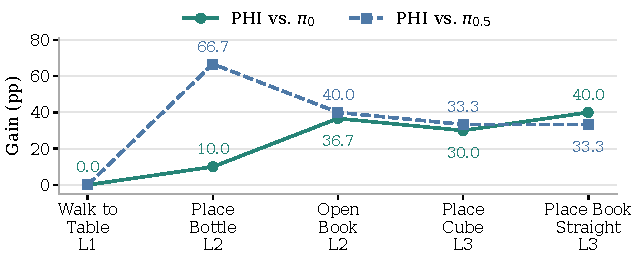
\includegraphics[width=\linewidth]{figures/gain_over_pi0.pdf}
%     \captionsetup{font=small,skip=2pt}
%     \caption{PHI's gains over $\pi_0$ and $\pi_{0.5}$ (pp).}
%     \label{fig:contact_gain}
% \end{wrapfigure}
% \paragraph{Robustness to Visual Distractors.}

\setlength{\intextsep}{2pt}
\begin{wrapfigure}[10]{r}{0.50\textwidth}
    \centering
    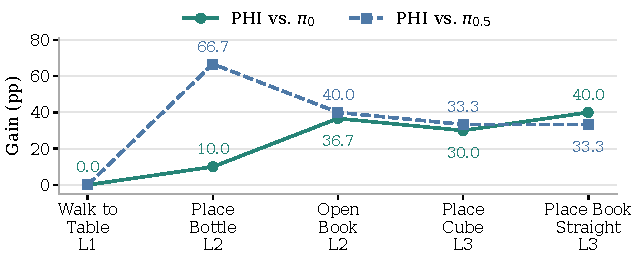
\includegraphics[width=\linewidth]{figures/gain_over_pi0.pdf}
    \captionsetup{font=small,skip=1pt}
    \caption{PHI's gains over $\pi_0$ and $\pi_{0.5}$.}
    \label{fig:contact_gain}
\end{wrapfigure}

\paragraph{Task-Specific Performance Gains.}
Figure~\ref{fig:contact_gain} summarizes the per-task gains. Across increasingly challenging tasks, PHI consistently exhibits larger gains over both baselines, particularly on contact-rich manipulation tasks. In contrast, all methods achieve $100\%$ on \textit{Walk to Table}, which requires no intentional hand–object contact. Figure~\ref{fig:qualitative_execution} (Appendix) shows selected successful PHI executions across the five tasks.

% \noindent
% \begin{minipage}{\linewidth}
%     \begin{minipage}[t]{0.38\linewidth}
%         \vspace{0pt}
%         % \textbf{Contact-level comparison.}
%         Figure~\ref{fig:contact_gain} shows PHI's gains
%         over $\pi_0$ and $\pi_{0.5}$.
%     \end{minipage}
%     \hfill
%     \begin{minipage}[t]{0.61\linewidth}
%         \vspace{0pt}
%         \centering
%         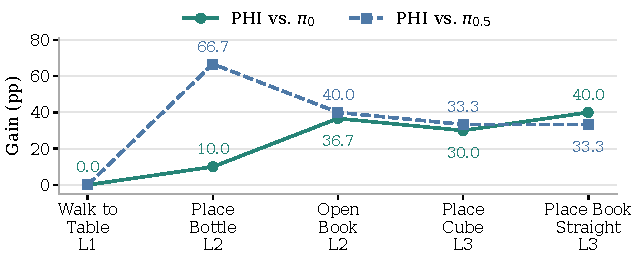
\includegraphics[width=\linewidth]{figures/gain_over_pi0.pdf}
%         \captionsetup{font=small,skip=2pt}
%         \captionof{figure}{PHI's gains over $\pi_0$ and $\pi_{0.5}$ (pp).}
%         \label{fig:contact_gain}
%     \end{minipage}
% \end{minipage}

% The two bimanual book tasks provide a focused comparison of performance on sustained-support and sliding-and-rotation manipulation. On \textit{Open Book}, PHI achieves $86.7\%$ success, compared with $50.0\%$ for $\pi_0$ and $46.7\%$ for $\pi_{0.5}$. 
% On \textit{Place Book Straight}, PHI achieves $76.7\%$ success, compared with $43.3\%$ for $\pi_{0.5}$ and $36.7\%$ for $\pi_0$. 
% PHI also outperforms the baselines on the two unimanual object-placement tasks, \textit{Place Bottle} and \textit{Place Cube}. On \textit{Place Bottle}, PHI achieves $76.7\%$ success, compared with $66.7\%$ for $\pi_0$ and $10.0\%$ for $\pi_{0.5}$. On \textit{Place Cube}, PHI achieves $70.0\%$ success, compared with $40.0\%$ for $\pi_0$ and $36.7\%$ for $\pi_{0.5}$. On \textit{Walk to Table}, which requires no intentional hand--object contact, PHI, $\pi_0$, and $\pi_{0.5}$ all achieve $100\%$ success; no additional gain over these two baselines is observed under this evaluation. Figure~\ref{fig:contact_gain} summarizes the per-task gains over $\pi_0$ and $\pi_{0.5}$.

% First, PHI, $\pi_0$, and $\pi_{0.5}$ all achieve $100\%$ success on the no-contact \textit{Walk to Table} task, 
% PHI achieves $70.0$--$86.7\%$ success and is the best-performing method in every case.
% Across all five tasks, PHI obtains an average success rate of $82.0\%$, 
% a \textbf{$39.7\%$ relative improvement} over the strongest baseline average of $58.7\%$ from $\pi_0$.

% Second, contact introduces failure modes that cannot be reliably resolved from visual observations alone. In \textit{Place Bottle}, the robot must grasp and transport the bottle without applying excessive or unstable contact forces that may knock the bottle over. This makes stable grasping and force regulation critical even though the task itself does not require complex bimanual manipulation. PHI achieves $76.7\%$ success, substantially outperforming $\pi_{0.5}$ ($10.0\%$) and $\pi_0$ ($66.7\%$). The larger gap over $\pi_{0.5}$ suggests that contact-sensitive manipulation can be particularly challenging for policies relying primarily on visual observations.

% \textit{Place Cube} requires a unimanual grasp-and-place of a small cube. The policy must precisely control the grasp location to avoid inducing unwanted rotation, while modulating fingertip pinch force to regulate friction so that the cube does not slip. PHI achieves $70.0\%$ success, compared with $40.0\%$ for $\pi_0$ and $36.7\%$ for $\pi_{0.5}$.

% The difficulty increases substantially in \textit{Open Book}, where successful execution requires accurate placement of both hands, coordinated bimanual motion, and appropriate regulation of the interaction forces. The robot must simultaneously lift the cover with one hand and stabilize the book with the other, making small errors in either hand position or applied force sufficient to cause failure. PHI achieves $86.7\%$ success, compared with $50.0\%$ for $\pi_0$ and $46.7\%$ for $\pi_{0.5}$.

% Finally, \textit{Place Book Straight} requires the policy to adapt to the book's initial pose: in some configurations a single sliding motion is sufficient, while others require translating the book and then rotating it to the target pose. PHI achieves $76.7\%$ success, substantially higher than $\pi_{0.5}$ ($43.3\%$) and $\pi_0$ ($36.7\%$).






\subsection{Generalization to Unseen Objects and Visual Conditions}
\label{sec:generalization}

% We next evaluate whether PHI can generalize beyond the visual and physical conditions observed during training. We consider two types of distribution shifts: visual distractors that change the scene composition, and unseen objects that change both object appearance and physical interaction properties. These experiments test whether the policy can adapt to the underlying manipulation state rather than relying on memorized visual patterns.
% We first evaluate the robustness of PHI to changes in scene composition. During evaluation, several irrelevant objects with different appearances are placed around the target object, while the manipulation objective and target object remain unchanged. The identities and positions of the distractors are varied across trials, preventing the policy from relying on a fixed scene layout.
% As shown in Fig.~\ref{fig:generalization}(a), PHI maintains a high success rate under visual clutter, achieving $70.0\%$ (7/10) compared with $30.0\%$ (3/10) for $\pi_0$ and $10.0\%$ (1/10) for $\pi_{0.5}$. Relative to the in-domain rate of $76.7\%$ (23/30), this is a drop of 6.7 percentage points on a smaller 10-trial evaluation. The scenes below panel (a) show one in-domain layout and three clutter examples.

% We next evaluate PHI under visual and physical conditions
% that differ from those observed during training.
% We consider two types of distribution shifts:
% visual distractors that change the scene composition,
% and unseen objects that differ in appearance and
% physical interaction properties.
% These experiments assess task performance under changes
% in scene composition and object identity.

We next evaluate PHI under visual and physical distribution shifts in scene composition and object identity. Specifically, we consider visual distractors that alter scene composition and unseen objects that differ in appearance and physical interaction properties.

\paragraph{Robustness to Visual Distractors.}
We evaluate PHI under changes in scene composition by placing irrelevant objects with varying appearances and positions around the target object, while keeping the target and manipulation objective unchanged. As shown in Fig.~\ref{fig:generalization}(a), PHI achieves $70.0\%$ success under visual clutter, compared with $30.0\%$ for $\pi_0$ and $10.0\%$ for $\pi_{0.5}$, versus $76.7\%$ in-domain. 
% The corresponding $95\%$ Wilson confidence intervals are $39.7\%$–$89.2\%$ and $59.1\%$–$88.2\%$, respectively. 
The scenes below panel (a) show one in-domain layout and three clutter examples.

% We evaluate PHI under changes in scene composition by
% placing several irrelevant objects with different
% appearances around the target object, while keeping
% the target object and manipulation objective unchanged.
% Distractor identities and positions vary across trials
% to test transfer across varied scene layouts.
% As shown in Fig.~\ref{fig:generalization}(a), PHI achieves
% $70.0\%$ success under visual clutter, compared
% with $30.0\%$ for $\pi_0$ and $10.0\%$
% for $\pi_{0.5}$.
% For reference, PHI achieves $76.7\%$ in-domain.
% The corresponding $95\%$ Wilson confidence intervals
% are $39.7\%$--$89.2\%$ under clutter and
% $59.1\%$--$88.2\%$ in-domain.
% PHI has the highest observed success rate among the
% evaluated methods under clutter, although the small
% sample size limits the precision of this comparison.
% The scenes below panel (a) show one in-domain layout
% and three clutter examples.

\paragraph{Generalization to Unseen Objects.}
We further evaluate object-level generalization using three books that never appear in the training data: \textit{Linear Algebra Done Right}, \textit{Federated Learning}, and \textit{Deep Learning}. The held-out books differ from the training objects in cover appearance, thickness, and material properties, including compliance. These variations introduce both visual and physical distribution shifts, as changes in thickness and compliance can alter the forces and contact conditions required for grasping, bracing, sliding, and opening. We evaluate both \textit{Place Book Straight} and \textit{Open Book} using the same three held-out books, with 10 trials per book. As shown in Fig.~\ref{fig:generalization}(b,c), PHI achieves $60.0\%$ success on \textit{Place Book Straight}, compared with $30.0\%$ for $\pi_{0.5}$ and $23.3\%$ for $\pi_0$, and $56.7\%$ on \textit{Open Book}, compared with $33.3\%$ for both baselines. These results correspond to absolute improvements of $30.0$ and $23.4$ percentage points over the strongest baseline, respectively. Together with the visual-distractor experiments, these results show that PHI generalizes to changes in scene composition, object identity, and physical properties. This suggests that its future representations capture task-relevant information for manipulation under varied visual and physical conditions.

% We further evaluate object-level generalization using three books that never appear in the training data: \textit{Linear Algebra Done Right}, \textit{Federated Learning}, and \textit{Deep Learning}. The held-out books differ from the training objects in cover appearance, thickness, and material properties, with one book being a softcover rather than a hardcover. These variations introduce both visual and physical distribution shifts, since changes in thickness and compliance can alter the forces required for grasping, bracing, sliding, and opening. PHI retains an aggregate advantage on both tasks, These results support transfer to the evaluated books rather than robustness to every appearance or contact-property change.




% We evaluate both \textit{Place Book Straight} and \textit{Open Book} using the same three held-out books, with 10 trials per book. Figure~\ref{fig:generalization}(b,c) reports the 30-trial aggregate for each task. The scenes below each panel show the seen book followed by the three held-out books. On \textit{Place Book Straight}, PHI achieves $60.0\%$ success (18/30), compared with $30.0\%$ for $\pi_{0.5}$ and $23.3\%$ for $\pi_0$, a $100\%$ relative improvement over the strongest baseline. On \textit{Open Book}, PHI reaches $56.7\%$ (17/30), while both $\pi_0$ and $\pi_{0.5}$ achieve $33.3\%$, a $70.0\%$ relative improvement.
%有点流水账，可以直接在表格看出来的不必要重复



\begin{figure}[h]
    \centering
    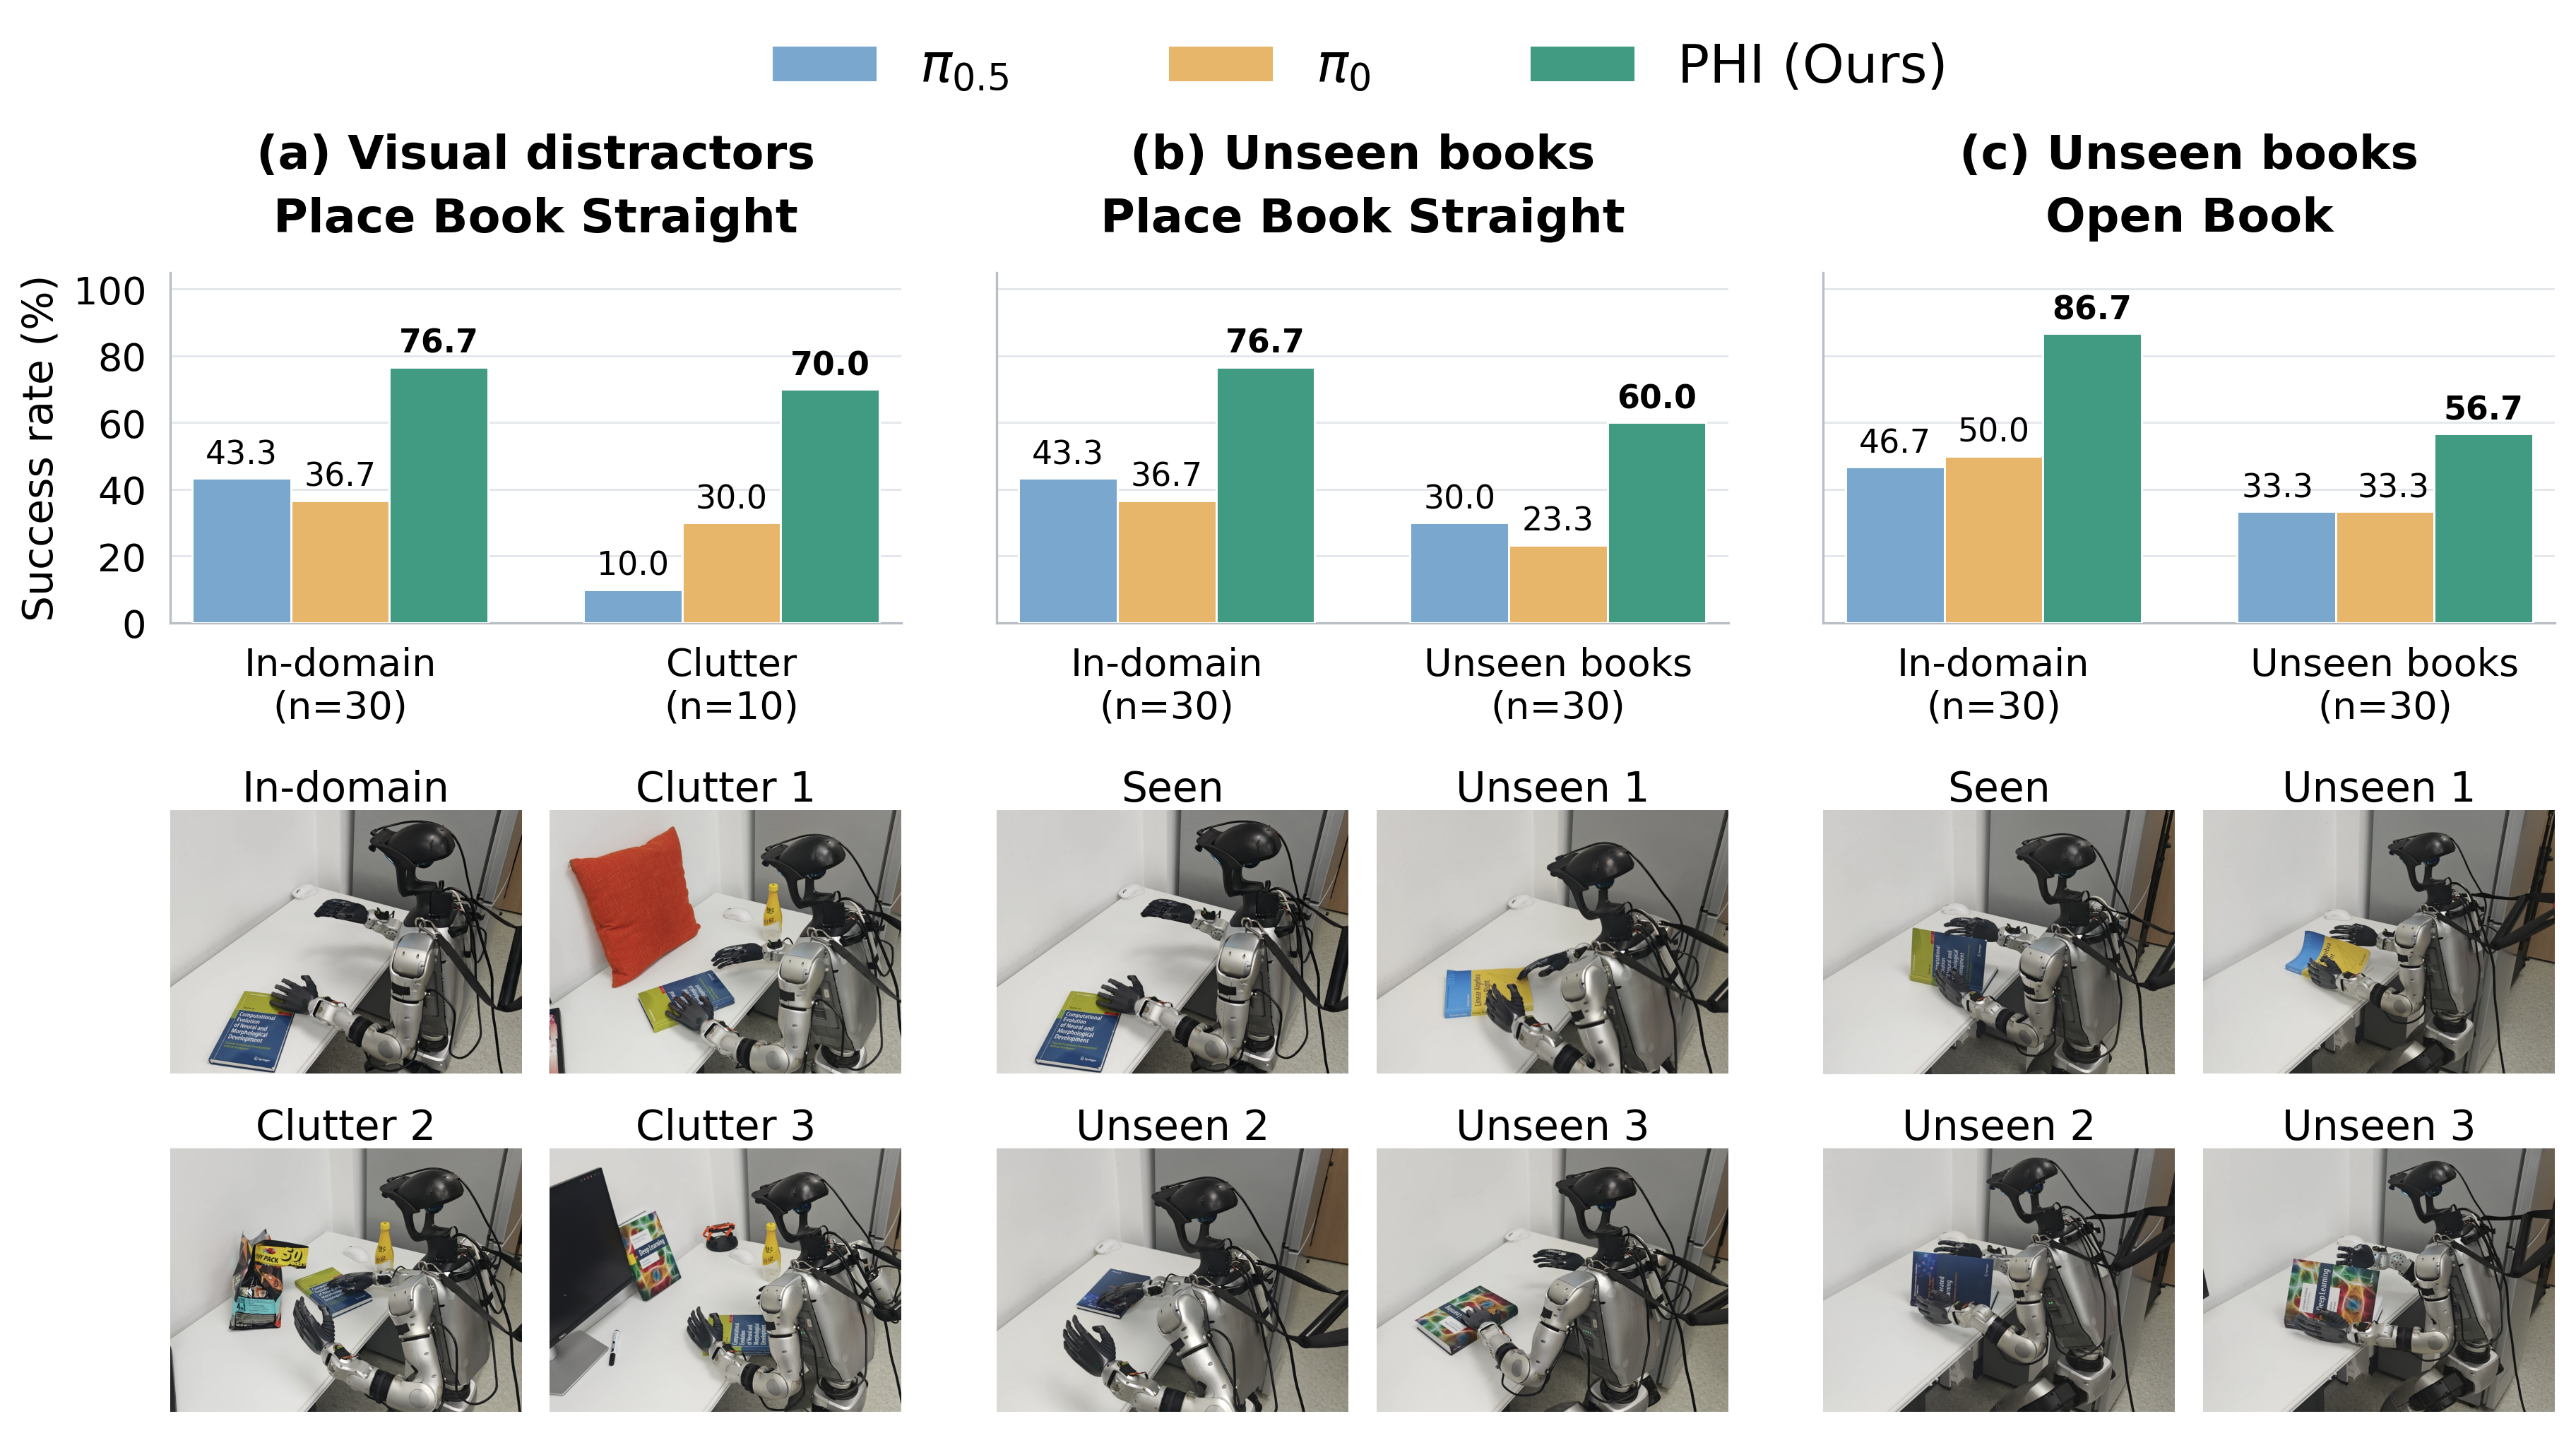
\includegraphics[width=\linewidth]
    {figures/generalization_combined.png}
    \caption{
    Generalization to visual distractors and unseen books.
    % (a) \textit{Place Book Straight} under clutter.
    % (b,c) Straightening and opening held-out books.
    }
    \label{fig:generalization}
\end{figure}


% \Needspace{20\baselineskip}
\subsection{Ablation Studies}
\label{sec:ablations}


We conduct ablation studies to examine the contributions
of temporal force conditioning and predictive future
latents. We evaluate both components on
 \textit{Place Book Straight},
which requires continuous contact, bimanual coordination,
and fine-grained interaction control. Each ablation
removes one component while keeping the remaining
architecture and training procedure unchanged.

% \noindent
% \begin{minipage}{\linewidth}
%     \begin{minipage}[t]{0.42\linewidth}
%         \vspace{0pt}
%         We conduct ablation studies to examine the contributions
%         of temporal force conditioning and predictive future
%         latents. We evaluate both components on
%         \textit{Open Book} and \textit{Place Book Straight},
%         which require continuous contact, bimanual coordination,
%         and fine-grained interaction control. Each ablation
%         removes one component while keeping the remaining
%         architecture and training procedure unchanged.
%     \end{minipage}
%     \hfill
%     \begin{minipage}[t]{0.55\linewidth}
%         \vspace{0pt}
%         \centering
%         \small
%         \setlength{\tabcolsep}{3pt}
%         \renewcommand{\arraystretch}{1.08}
%         \captionof{table}{Ablation success rates (\%) on two contact-rich tasks. Each variant removes one component while keeping the remaining architecture unchanged. Dashes indicate unreported results.}
%         \label{tab:ablations}
%         \begin{tabular}{@{}lcc@{}}
%             \toprule
%             \textbf{Variant}
%             & \shortstack{\textbf{Place Book}\\\textbf{Straight}}
%             & \shortstack{\textbf{Open}\\\textbf{Book}} \\
%             \midrule
%             \textbf{PHI} & \textbf{76.7} & \textbf{86.7} \\
%             w/o force conditioning & -- & -- \\
%             w/o predictive future latent & -- & -- \\
%             \bottomrule
%         \end{tabular}
%     \end{minipage}
% \end{minipage}
% \par\medskip

% \paragraph{Effect of Force Conditioning.}

% We first remove temporal force conditioning while keeping the visual observations and predictive future latent unchanged. As shown in Table~\ref{tab:ablations}, removing force conditioning degrades the performance on both contact-rich tasks. Without force information, the policy must infer the physical interaction state primarily from visual observations, making it difficult to determine whether contact has been successfully established, whether the applied force is sufficient for sliding, and when the interaction should stop. The degradation is particularly evident in \textit{Place Book Straight}, where successful execution requires continuous regulation of normal and tangential forces during sliding. These results demonstrate that temporal force information provides complementary state information that cannot be reliably recovered from vision alone.

% \paragraph{Effect of Temporal Force Encoding.}

% We remove the temporal force encoder and its dedicated history representation $z_t^f$, while retaining current force measurements in $s_t$ and keeping the visual observations and predictive future latent unchanged. Current force information therefore remains available through both the VLM state context and the projected robot state $z_t^s$. This ablation isolates the contribution of explicit force-history modeling beyond instantaneous force inputs. As shown in Table~\ref{tab:ablations}, removing temporal force encoding degrades performance on both contact-rich tasks. Without temporal force encoding, the policy lacks the dedicated representation of recent force evolution that can help distinguish contact establishment, sustained sliding, and interaction termination. The degradation is particularly evident in \textit{Place Book Straight}, where successful execution requires continuous regulation of normal and tangential forces during sliding. These results suggest that modeling force history provides useful information about contact dynamics beyond the current visual observations and instantaneous force measurements.


% \paragraph{Effect of Predictive Future Latents.}

% We next remove the predictive future latent while retaining force conditioning. This ablation evaluates whether explicitly anticipating future visual states provides benefits beyond current observations and force feedback. Removing the predictive component leads to degraded performance on both tasks, with more frequent delayed transitions, overshooting, and failures to appropriately switch between manipulation phases.

% The effect is particularly important for \textit{Place Book Straight}, where different initial poses can require different future action sequences. Depending on the initial configuration, the robot may only need to slide the book, or may need to translate it first and subsequently rotate it. 
% % A policy based only on the current observation and force state must infer the appropriate future action online, whereas the predictive latent provides an explicit representation of the expected future visual state.
% PHI explicitly conditions the policy on a predictive representation learned with future-observation supervision during training. At deployment, this representation is inferred solely from the currently available interaction context and may help distinguish subsequent manipulation phases; it does not provide access to actual future observations.
%缩短版
\paragraph{Effect of Temporal Force Encoding.}

% \begin{wraptable}{r}{0.4\textwidth}
%     \centering
%     \small
%     \setlength{\tabcolsep}{5pt}
%     \renewcommand{\arraystretch}{1.08}
%     \captionsetup{font=small,skip=4pt}
%     \caption{Ablation success rates (\%).}
%     \label{tab:ablations}
%     \begin{tabular}{@{}lcc@{}}
%         \toprule
%         \textbf{Variant}
%         & \shortstack{\textbf{Place Book}\\\textbf{Straight}} \\
%         \midrule
%         \textbf{PHI} & \textbf{76.7}  \\
%         w/o force conditioning & 63.3(19/30)  \\
%         w/o predictive future latent & 50.0(15/30)  \\
%         \bottomrule
%     \end{tabular}
% \end{wraptable}
\setlength{\intextsep}{2pt}

\begin{wraptable}{r}{0.4\textwidth}
    \centering
    \small
    \setlength{\tabcolsep}{5pt}
    \renewcommand{\arraystretch}{1.08}
    \captionsetup{font=small,skip=4pt}
    \caption{Ablation success rates (\%).}
    \label{tab:ablations}
    \begin{tabular}{@{}lcc@{}}
        \toprule
        \textbf{Variant}
        & \shortstack{\textbf{Place Book}\\\textbf{Straight}} \\
        \midrule
        \textbf{PHI} & \textbf{76.7}(23/30)  \\
        w/o Temporal Force Encoder & 63.3(19/30)  \\
        w/o Future Learning Module & 50.0(15/30)  \\
        \bottomrule
    \end{tabular}
\end{wraptable}
We remove the temporal force encoder and its history representation $z_t^f$, while retaining the current force measurements in $s_t$ and keeping the Future Learning module
$\mathcal{T}_{\phi}$ unchanged. As shown in Table~\ref{tab:ablations}, this leads to a $13.4$ percentage points drop on \textit{Place Book Straight}, which requires continuous force regulation during sliding. Without force modeling, the robot more frequently fails to move the book because the fingers either fail to establish contact or press the book too tightly. However, the overall manipulation behavior remains correct, resulting in a relatively limited drop in success rate. This suggests that force-history modeling mainly improves contact regulation during execution rather than action planning. The force traces for all tasks are provided in Fig.~\ref{fig:tactile_traces} (Appendix).
% We remove the temporal force encoder and its dedicated history representation $z_t^f$, while retaining current force measurements in $s_t$ and keeping the visual observations and predictive future latent unchanged. This isolates the contribution of explicit force-history modeling beyond instantaneous force inputs. As shown in Table~\ref{tab:ablations}, removing temporal force encoding degrades performance on both contact-rich tasks, particularly \textit{Place Book Straight}, which requires continuous regulation of normal and tangential forces during sliding. Without temporal force encoding, the policy lacks explicit information about recent force evolution, making it harder to distinguish contact establishment, sustained sliding, and interaction termination. These results indicate that force history provides useful information about contact dynamics beyond instantaneous force measurements.

\paragraph{Effect of Predictive Future Latents.}
We remove the Future Learning module $\mathcal{T}_{\phi}$ while retaining force conditioning. As shown in Table~\ref{tab:ablations}, this causes a $26.7$ percentage points drop on \textit{Place Book Straight}. In our experiments, the robot shows clear degradation in manipulation planning: after moving the book into position, it often stalls when a subsequent rotation is required or rotates in the wrong direction. These results show that the future features extracted by our module provide useful information for planning subsequent actions and selecting appropriate manipulation behaviors.

% We remove the Future Learning module
% $\mathcal{T}_{\phi}$ while retaining force conditioning to evaluate the benefit of anticipating future visual states beyond current observations and force feedback. As shown in Table~\ref{tab:ablations}, performance degrades on both tasks, with more frequent delayed transitions, overshooting, and failures in switching between manipulation phases. The effect is particularly evident in \textit{Place Book Straight}, where different initial poses may require sliding directly or first translating and then rotating the book. By conditioning the policy on a predictive representation learned from future-observation supervision during training, PHI provides information about subsequent manipulation phases without accessing future observations at deployment.





% Figure~\ref{fig:latent_analysis} presents a single-sample visualization of predicted and target future-latent tokens for one exported frame, with the target representation extracted from five future stereo observations. The predicted and target tokens are jointly projected onto a shared PCA basis fitted to their concatenation. The first two principal components explain $36.7\%$ and $21.2\%$ of the variance in this sample's pooled tokens, respectively. Diamonds and triangles denote target and predicted tokens, and lines connect matching query pairs. Predicted tokens are colored by per-query mean squared error, averaged over the 2048 feature dimensions in the original representation space. The reported cosine similarity of $0.9690$ is computed in the original feature space for each matched predicted--target token pair and then averaged over the 512 queries in this sample. It indicates within-sample representation agreement, rather than average prediction quality across the test set, and does not by itself establish that the model captures contact transitions or improves action quality. Figure~\ref{fig:latent_alignment} further reports per-query original-space errors for this same sample.

%缩减版
% Figure~\ref{fig:latent_analysis} Presents a single-sample visualization of predicted and target future-latent tokens for one exported frame, with the target representation extracted from five future stereo observations. Both representations are projected onto a shared PCA basis fitted to their concatenation. The first two principal components explain $36.7\%$ and $21.2\%$ of the variance, respectively. Diamonds and triangles denote target and predicted tokens, with lines connecting matching query pairs. Predicted tokens are colored by per-query mean squared error averaged over the 2048 feature dimensions. The cosine similarity of $0.9690$ is computed in the original feature space for each matched pair and averaged over 512 queries. It reflects within-sample representation agreement rather than average prediction quality across the test set, and does not by itself establish that the model captures contact transitions or improves action quality. 

\paragraph{Future-Latent Alignment.}
Figure~\ref{fig:latent_analysis} visualizes predicted and target future-latent tokens. The target is extracted from five future stereo observations, and both features are projected onto a shared principal component analysis (PCA) basis. The first two components explain $36.7\%$ and $21.2\%$ of the total variance, respectively. Diamonds and triangles denote target and predicted tokens, with lines connecting matched queries; colors indicate per-query MSE over 2048 feature dimensions. The average cosine similarity is $0.9690$ across 512 queries, indicating strong alignment between the predicted and target features. Figure~\ref{fig:latent_alignment}(Appendix) further reports per-query original-space errors for the same sample.

\begin{figure}[h]
    \centering
    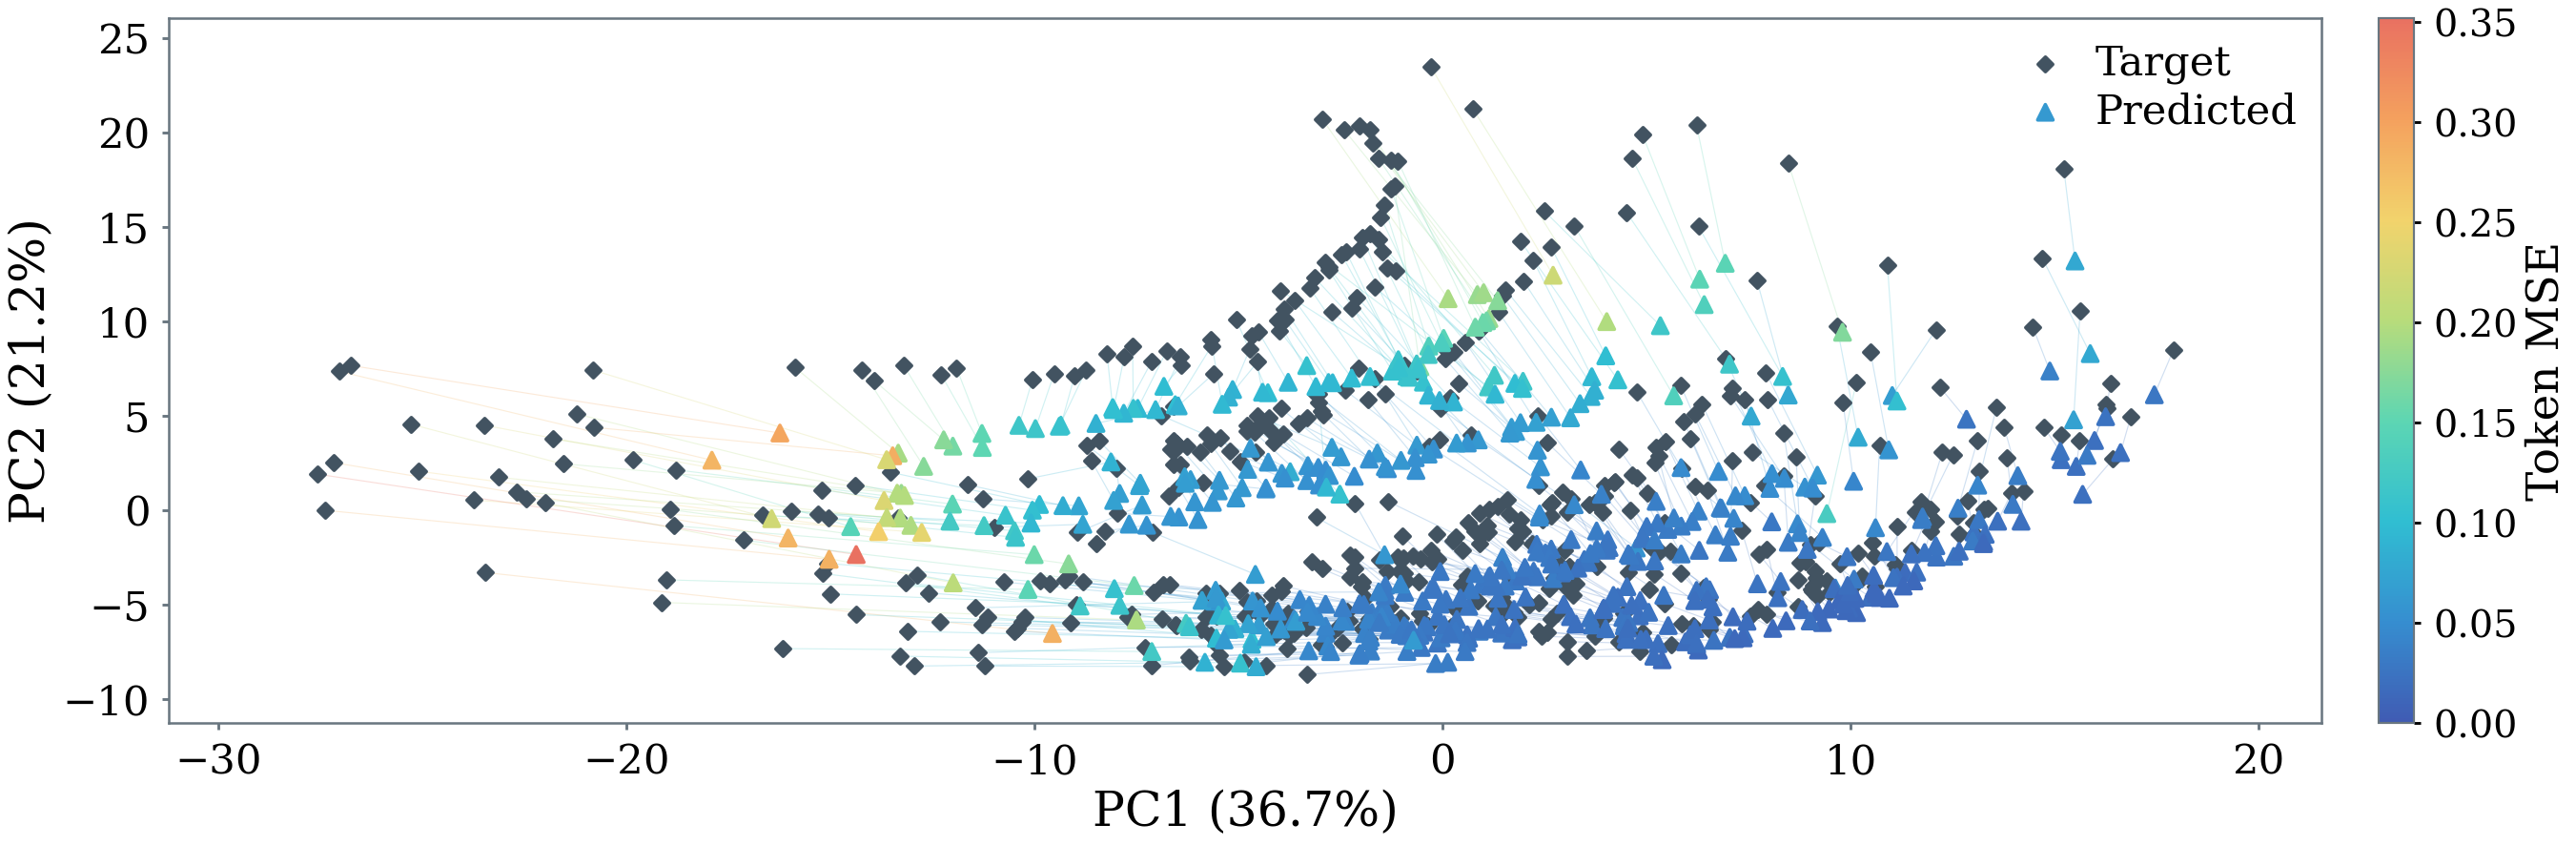
\includegraphics[width=.80\linewidth]{figures/PCA.png}
    \caption{Joint PCA of predicted and target future-latent tokens for a single exported frame. Lines connect matched queries; colors indicate per-query MSE in the original feature space.}
    \label{fig:latent_analysis}
\end{figure}


% To further understand this behavior, Fig.~\ref{fig:latent_analysis} presents a joint PCA visualization of the predicted and target future-latent tokens, with the target representation extracted from five future stereo observations. Both sets are projected into a shared two-dimensional space, where the first two principal components explain $36.7\%$ and $21.2\%$ of the total variance, respectively. Diamonds and triangles denote target and predicted tokens, lines connect matching query pairs, and predicted tokens are colored by their mean squared error in the original feature space. The predicted and target representations exhibit similar overall distribution patterns, consistent with a mean cosine similarity of $0.9690$. Original-space errors are further reported in Fig.~\ref{fig:latent_alignment}.

% We additionally visualize the attention maps of the action prediction network in Fig.~\ref{fig:attention_analysis}. The policy primarily attends to the manipulated object and the interacting hands, indicating that the learned representation focuses on regions directly related to future action generation. Together, the ablation and qualitative analyses suggest that predictive future representations provide action-relevant information about the upcoming manipulation state, complementing the instantaneous physical-state information provided by force conditioning.
% Figure~\ref{fig:attention_analysis} visualizes the final-layer attention of the teacher Perceiver as it aggregates privileged future stereo observations to construct the training-time target representation. In the displayed example, attention is concentrated on the manipulated object and interacting hands, illustrating which visual regions the teacher emphasizes during target construction. These maps describe the training-only teacher pathway and do not establish a causal contribution of the attended regions to action outputs. PHI is designed to combine the resulting predictive visual representation with the recent force dynamics captured by the temporal force encoder; the effect on policy performance must be assessed through controlled ablations.


% \subsubsection*{Acknowledgments}
% Use unnumbered third level headings for the acknowledgments. All
% acknowledgments, including those to funding agencies, go at the end of the paper.

\section{Conclusion}

We presented PHI, a hierarchical World Action Model for humanoid bimanual dexterous manipulation. PHI learns future representations shaped by downstream action supervision and combines them with temporal force features for action generation. Real-robot experiments on the Unitree G1 demonstrate improved performance across bimanual manipulation tasks and distribution shifts, highlighting the value of task oriented future representations for humanoid manipulation.

\bibliography{iclr2027_conference}
\bibliographystyle{iclr2027_conference}

\appendix
\clearpage
\section{Appendix}
\subsection{Visualization of Main Results}
\label{app:main_results_visualization}



Figure~\ref{fig:main_results_visualization} visualizes the success rates reported in Table~\ref{tab:main_results} to facilitate comparison across methods and tasks. Figure~\ref{fig:qualitative_execution} presents representative PHI execution sequences captured from a third-person view across the five real-robot tasks: \textit{Walk to Table}, \textit{Place Bottle}, \textit{Open Book}, \textit{Place Cube}, and \textit{Place Book Straight}. The sequences show successful task completion across both locomotion and contact-rich bimanual manipulation, demonstrating consistent execution across the evaluated tasks.

\begin{figure}[htbp]
    \centering
    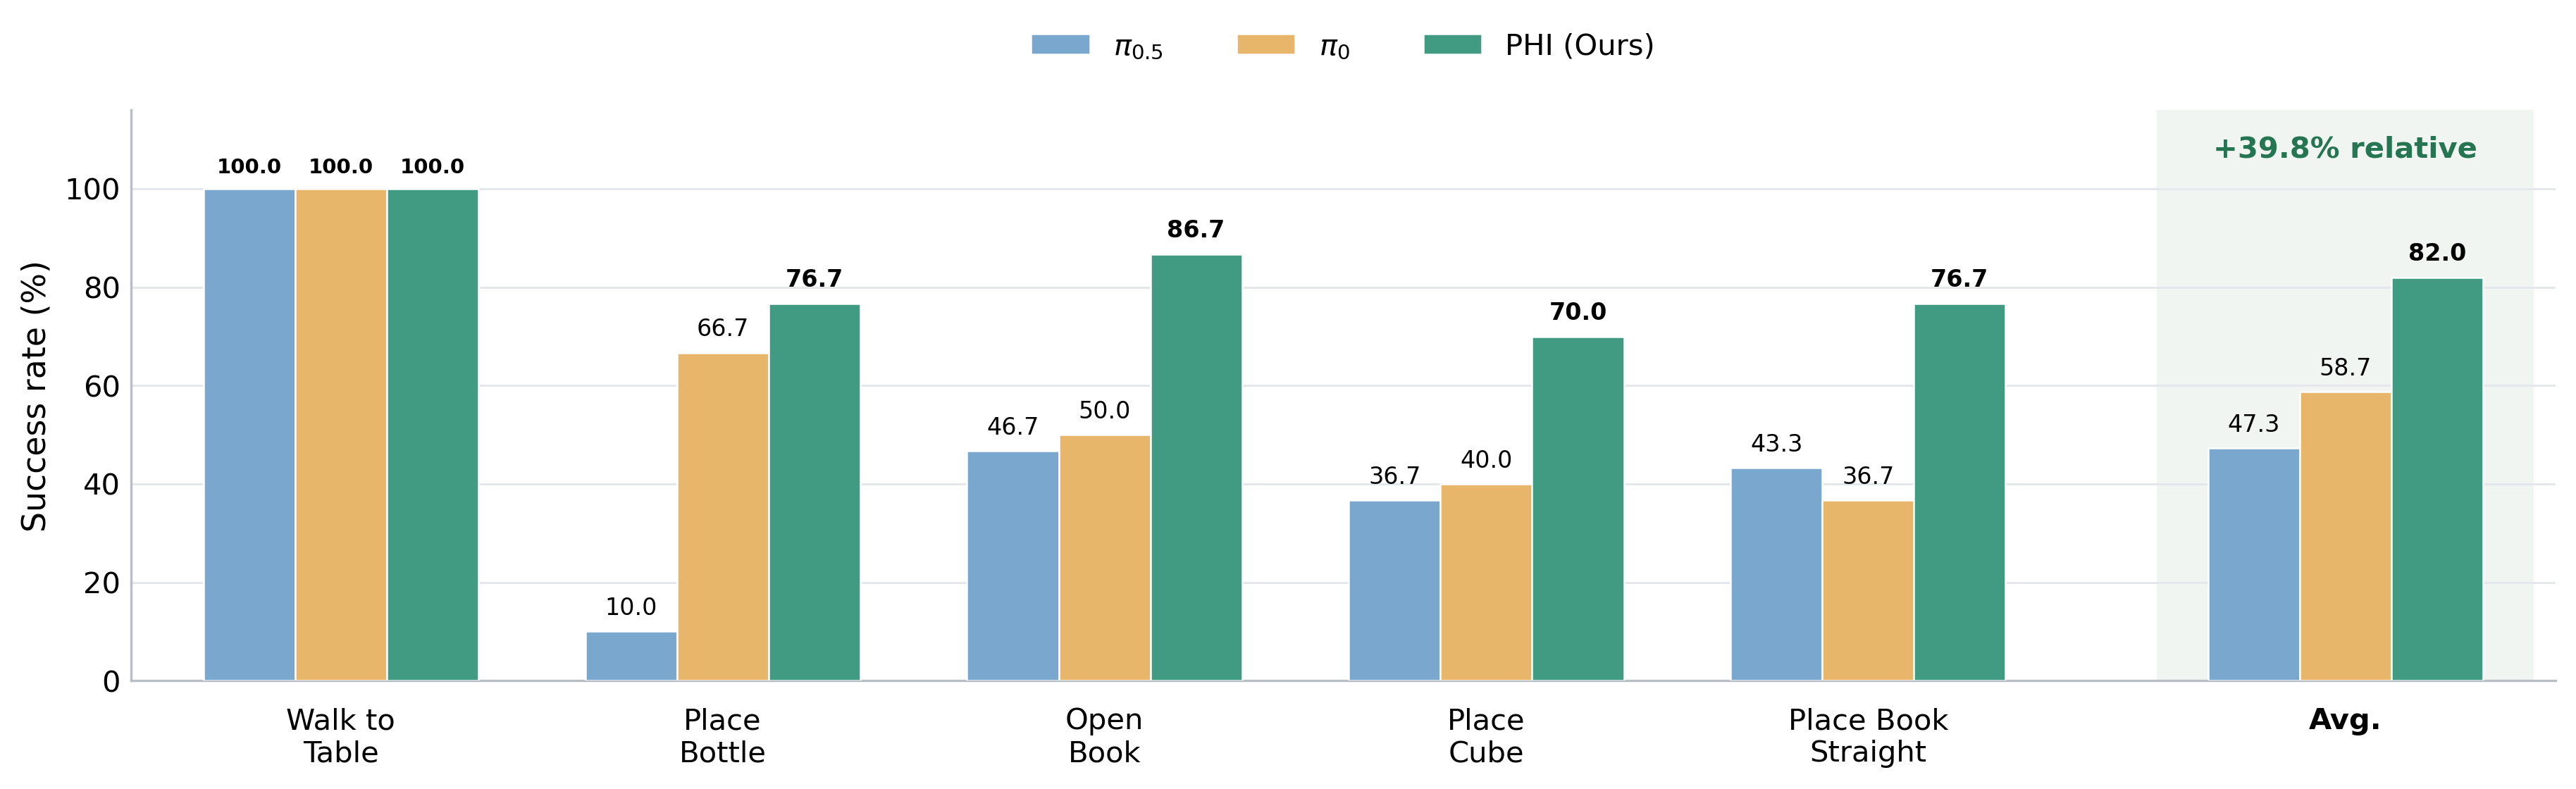
\includegraphics[width=\linewidth]
    {figures/main_results.png}
    \caption{
    Success rates across five real-robot tasks,
    with 30 trials per task and method.
    Avg.\ denotes the mean success rate across tasks.
    Bold labels indicate the best result in each column.
    }
    \label{fig:main_results_visualization}
\end{figure}

\begin{figure}[!tbh]
    \centering
    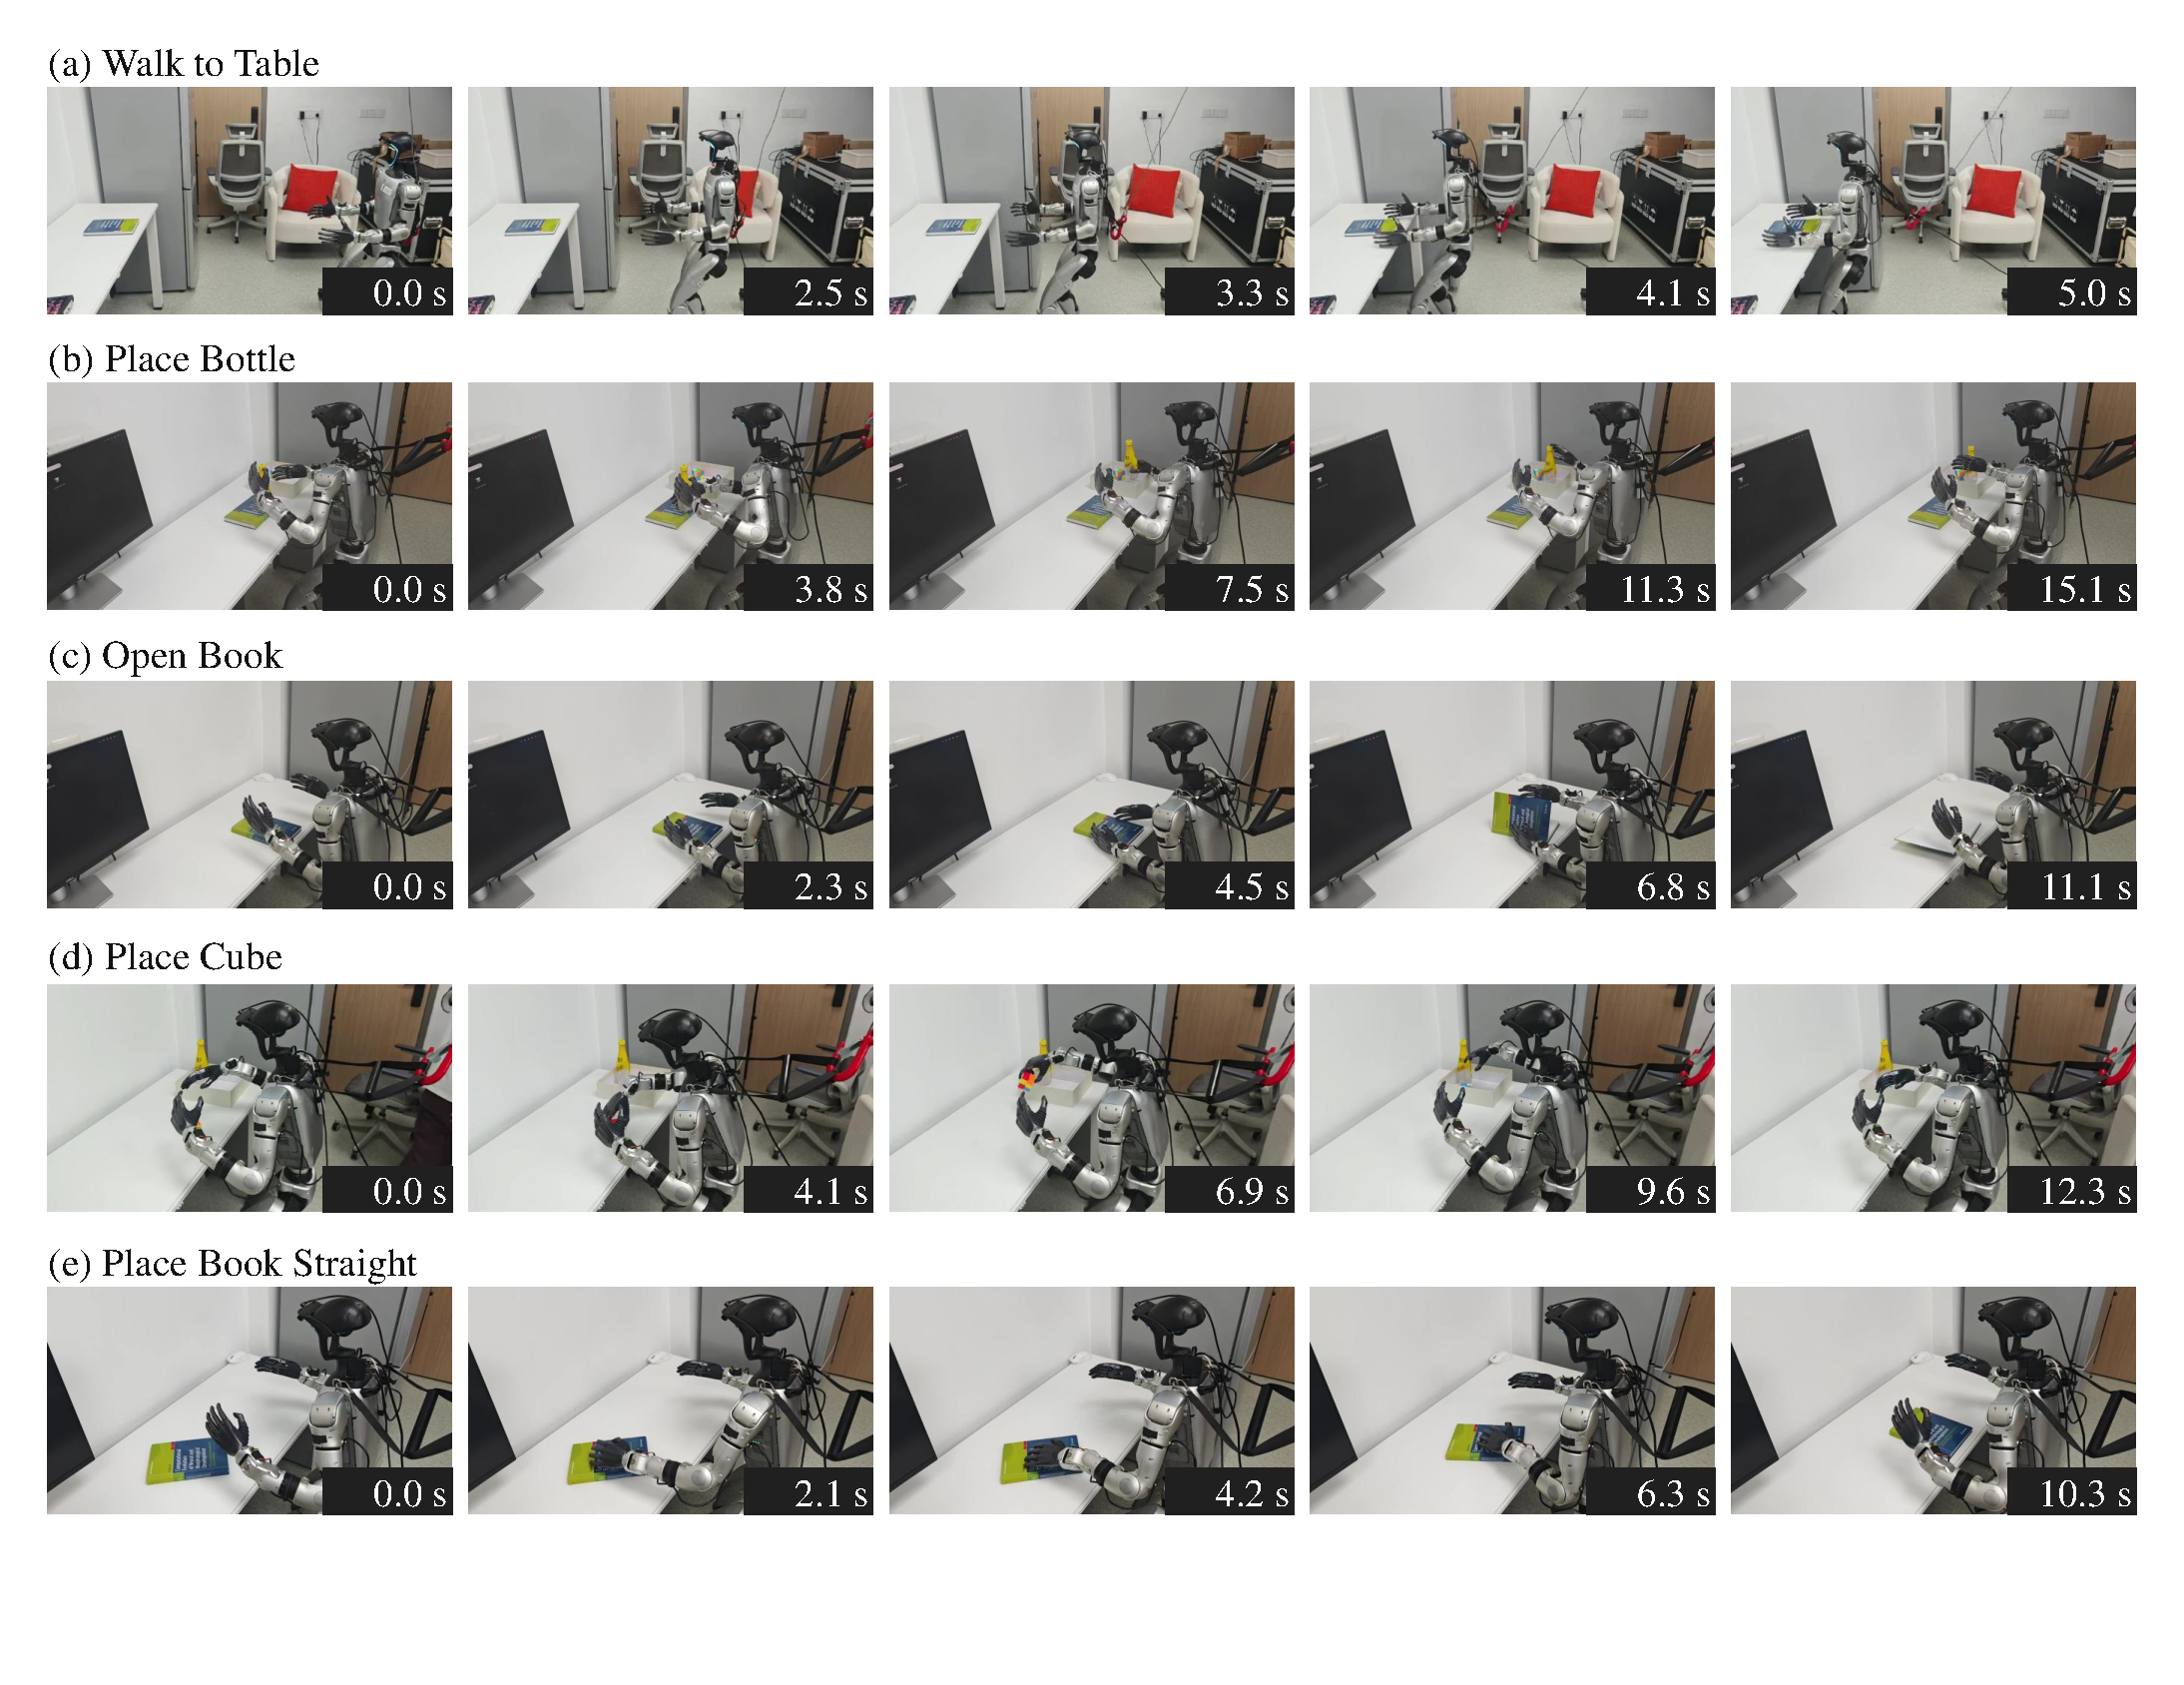
\includegraphics[width=\linewidth]{figures/qualitative_execution.pdf}
    \caption{Selected PHI execution sequences across the five tasks.}
    \label{fig:qualitative_execution}
\end{figure}



\subsection{Future-Target Attention and Alinement.}
Figure~\ref{fig:attention_analysis} visualizes the final-layer attention of the future Perceiver when aggregating privileged future stereo observations to construct the target representation. In the example, attention is concentrated on the manipulated object and interacting hands, indicating that the target representation emphasizes task-relevant visual regions for future manipulation. 

Figure~\ref{fig:latent_alignment} compares the predicted and target future representations for a single frame. In (a), the predicted latent is visualized across query tokens and pooled channels, while (b) shows the corresponding privileged target latent using the same color scale, allowing their feature patterns to be directly compared. In (c), the per-query MSE is computed in the original feature space to quantify the discrepancy between the two representations. The predicted and target latents exhibit similar feature patterns, with a mean MSE of $0.0632$ and a mean cosine similarity of $0.9690$, indicating that the predicted representation closely aligns with the privileged future target.

\begin{figure}[!tbh]
    \centering
    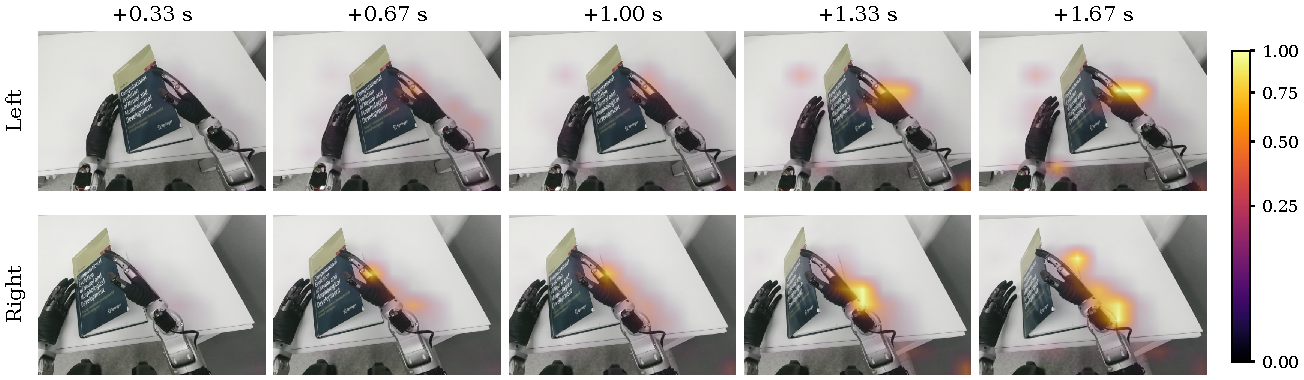
\includegraphics[width=.90\linewidth]{figures/perceiver_attention_focus.pdf}
    \caption{Final-layer attention of the future Perceiver over privileged future stereo observations, with rows denoting cameras and columns denoting future time offsets.}
    \label{fig:attention_analysis}
\end{figure}


\subsection{Tactile Traces During Task Execution}
\label{app:tactile_traces}

\begin{figure}[h]
    \centering
    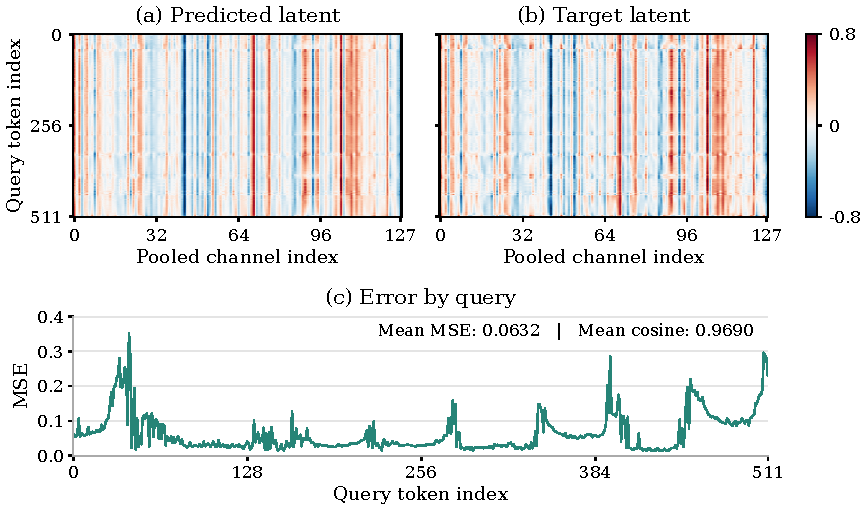
\includegraphics[width=\linewidth]{figures/latent_alignment_compact.pdf}
    \caption{Single-frame future-latent comparison.
    (a,b) Predicted and target representations with shared color limits,
    clipped at the pooled absolute-value 99.5th percentile.
    (c) Per-query MSE in the original feature space.}
    \label{fig:latent_alignment}
\end{figure}

Figure~\ref{fig:tactile_traces} shows selected successful execution segments for the five tasks, ordered from locomotion without object contact to contact-rich manipulation. Each row pairs the normal-force channels of both hands with five approximately equally spaced camera frames. Among these tasks, \textit{Place Book Straight} exhibits the most complex force variations. The robot first uses frictional contact with one hand to pull the book toward itself, and then uses frictional interactions with both hands to rotate and reorient the book. The corresponding force traces show distinct and coupled variations between the two hands, reflecting the changing contact conditions throughout the manipulation.

\begin{figure}[h]
    \centering
    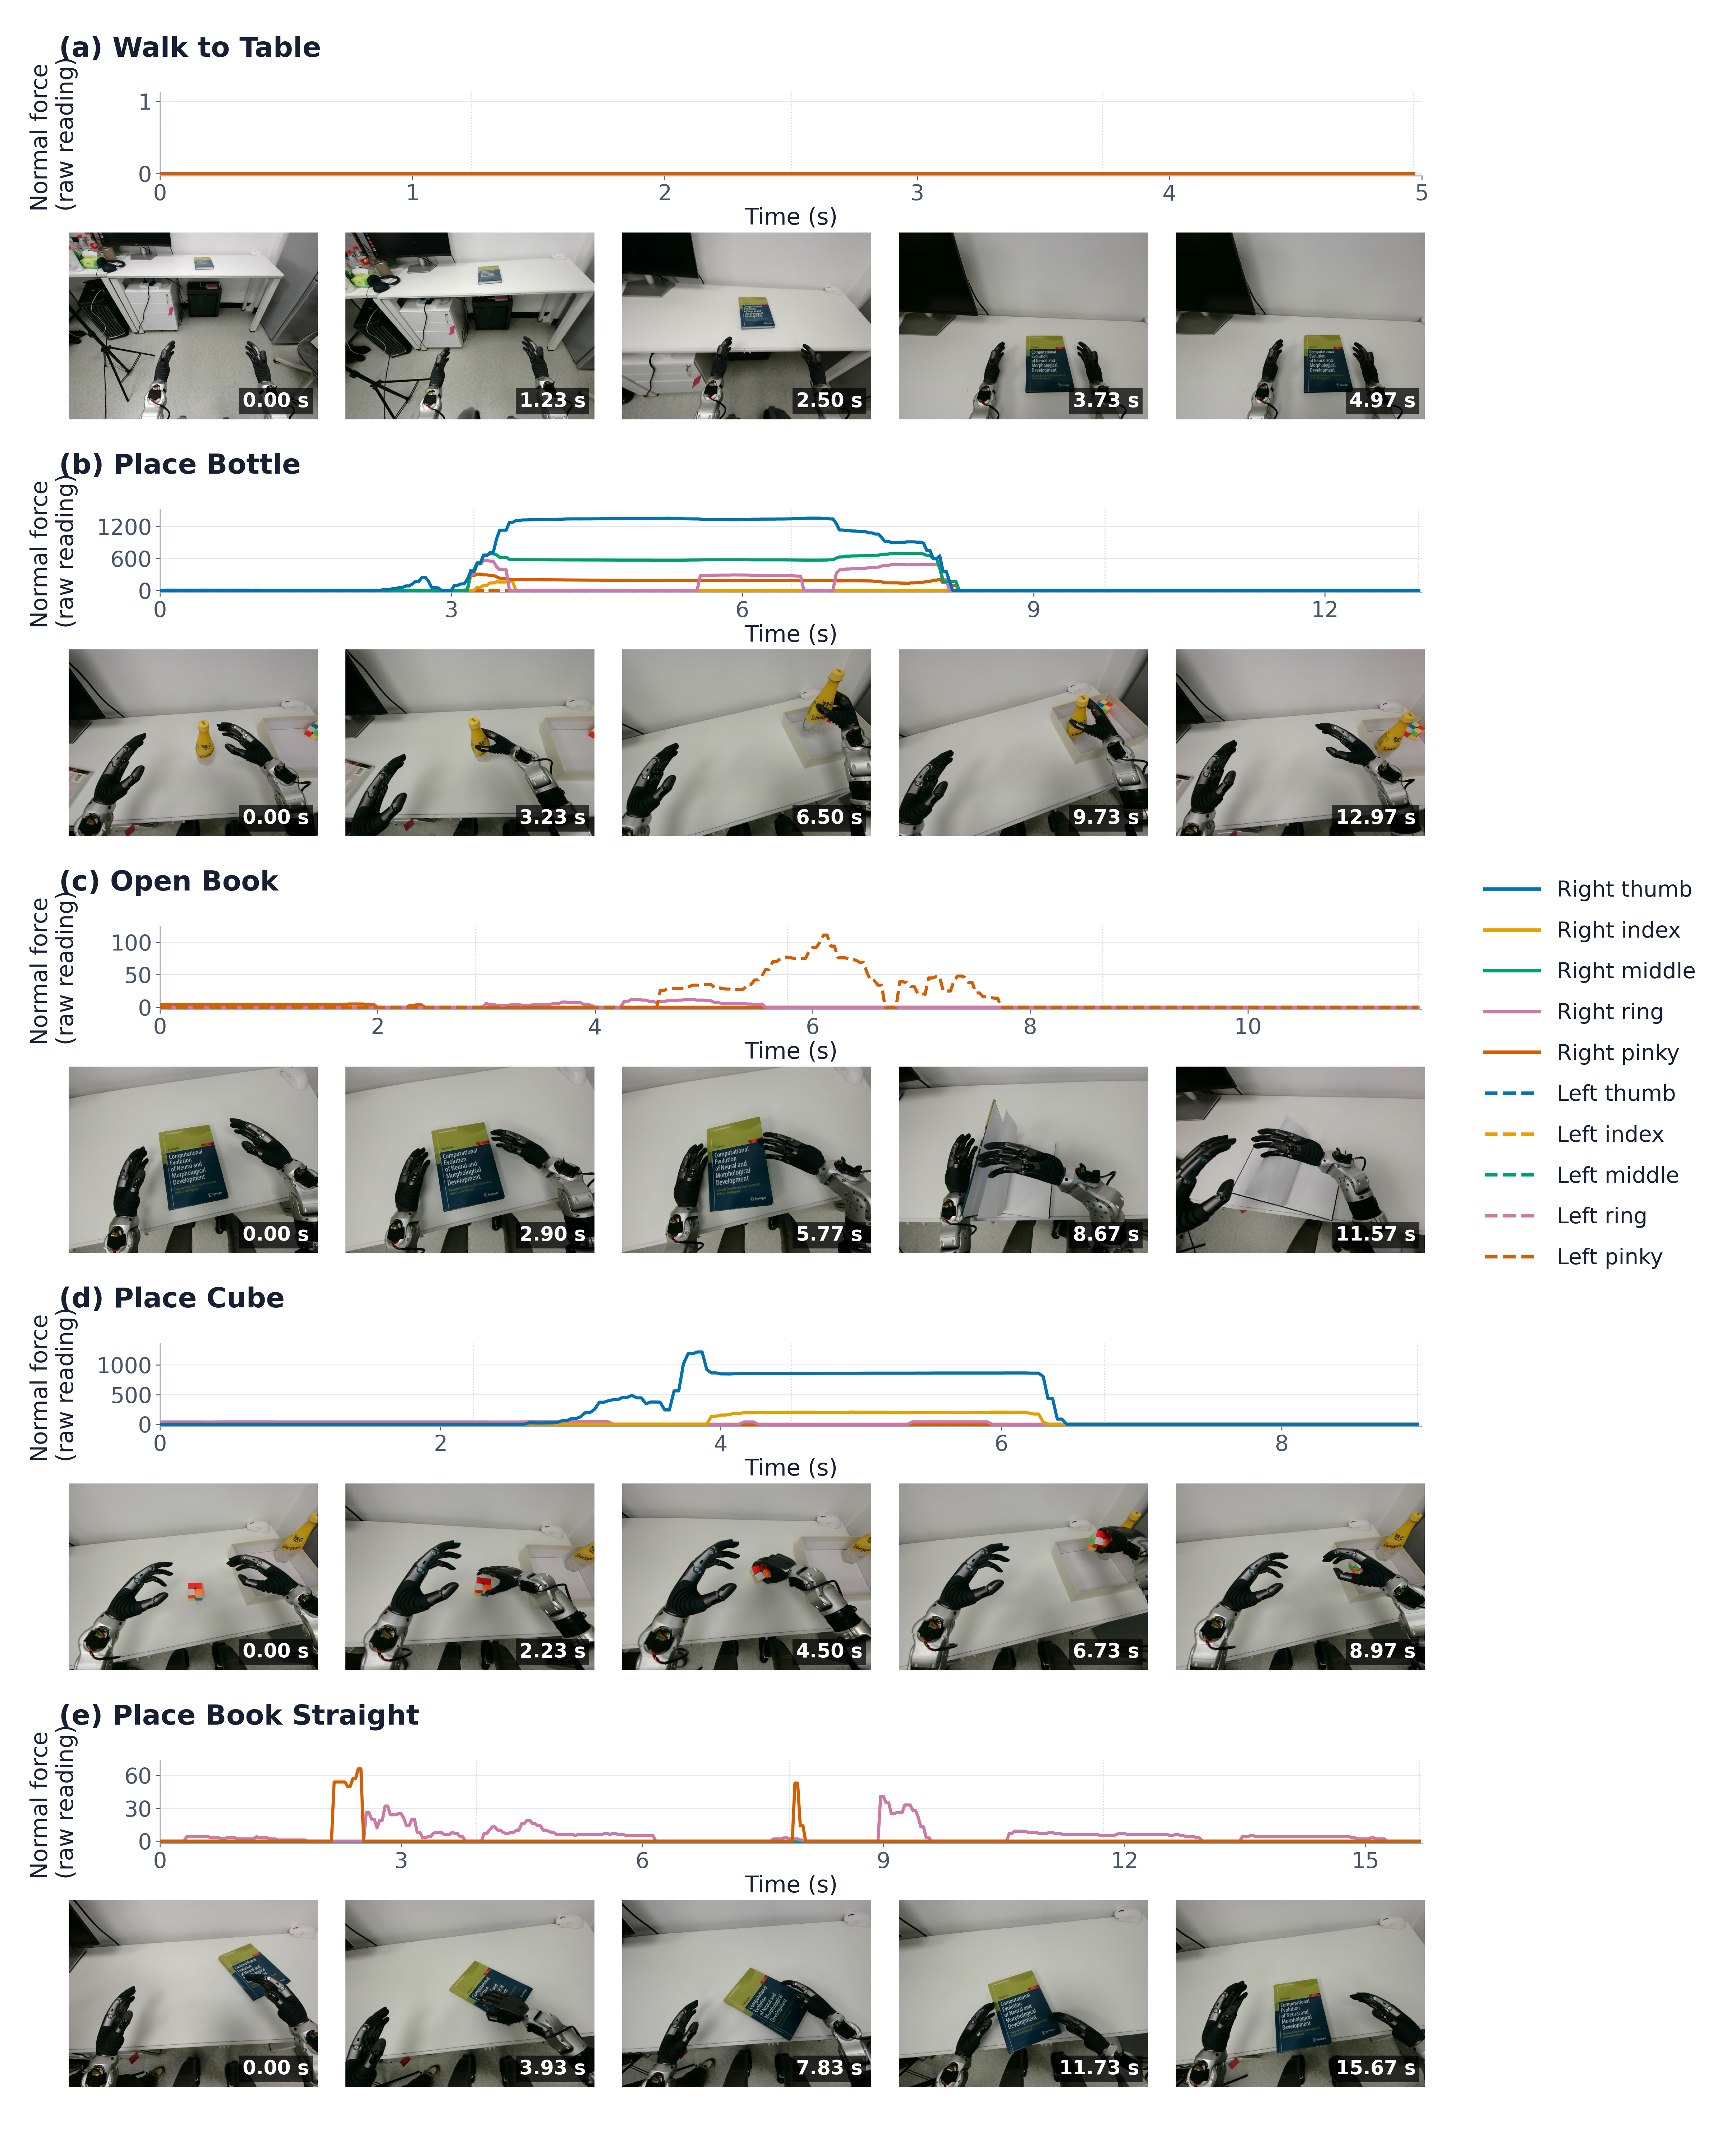
\includegraphics[width=\linewidth,height=.80\textheight,keepaspectratio]{figures/pressure_five_tasks_with_frames.png}
    \caption{Normal-force traces and corresponding camera frames for five selected execution segments.}
    \label{fig:tactile_traces}
\end{figure}





\subsection{Key Training Hyperparameters}
Table~\ref{tab:training_hyperparameters} summarizes the key training hyperparameters used for PHI, including the optimization settings, learning rates for different training stages, action and future-prediction loss weights, and model input and output configurations.

\begin{table}[h]
\centering
\small
\caption{Key training hyperparameters.}
\label{tab:training_hyperparameters}
\begin{tabular}{p{0.30\linewidth} p{0.62\linewidth}}
\toprule
\textbf{Hyperparameter} & \textbf{Setting} \\
\midrule
Batch size & 6 \\
Training steps & 500K \\
Maximum token length & 768 \\
Action chunk length & 50 \\
Action history length & 10 \\
Number of future frames / stride & 5 / 10 \\
Training precision & BFloat16 \\
\midrule
Stage I learning rates &
WAM: $5\times10^{-5}$;
vision encoder: $2.5\times10^{-5}$;
future resampler: $5\times10^{-5}$;
action expert: $5\times10^{-5}$ \\
Stage II learning rates &
WAM: $5\times10^{-5}$; \\
Stage III learning rates &
WAM: $2.5\times10^{-5}$;
action expert: $1\times10^{-5}$ \\
\midrule
Action loss weights &
$\lambda_{\mathrm{arm}}=1.5$,
$\lambda_{\mathrm{hand}}=2.0$,
$\lambda_{\mathrm{move}}=0.5$ \\
Future loss weight &
$\lambda_{\mathrm{future}}=1.0$ (Stage II); 
$\lambda_{\mathrm{future}}=0.1$ (Stage III) \\
\midrule
Optimizer &
AdamW, $\beta_1=0.9$, $\beta_2=0.95$,
weight decay $=0.01$ \\
Learning-rate schedule &
1,000-step warmup, cosine decay, gradient clipping $=1.0$ \\
\bottomrule
\end{tabular}
\end{table}

\end{document}



